\documentclass[letterpaper,11pt,leqno]{article}

% ========== INTEGRATED PREAMBLE (formerly paper.sty) ==========

% ---------- Fonts ----------
%\usepackage{sourceserifpro}
\usepackage[T1]{fontenc}
\usepackage{amsmath,amssymb,amsthm,eucal,bbold,bm}
\usepackage[italic,eulergreek]{mathastext}
\input{glyphtounicode}\pdfgentounicode=1

\usepackage{tabularx}

% ---------- Spacing ----------
\usepackage{setspace}
\setstretch{1.35}
\renewcommand{\floatpagefraction}{0}
\AtBeginDocument{\allowdisplaybreaks[1]}

% ---------- TikZ Graphics ----------
\usepackage{tikz}
\usepackage{verbatim}
\usetikzlibrary{positioning}
\usetikzlibrary{snakes}
\usetikzlibrary{calc}
\usetikzlibrary{arrows}
\usetikzlibrary{decorations.markings}
\usetikzlibrary{shapes.misc}
\usetikzlibrary{matrix,shapes,arrows,fit,tikzmark}
\usetikzlibrary{decorations.pathreplacing}

\tikzset{
    pics/noedge/.style={
        code={
            \draw[pic actions] (-#1,-#1) -- (#1,#1);
            \draw[pic actions] (-#1,#1) -- (#1,-#1);
        }
    },
    noedge/.default=0.2cm
}

% ---------- General Typography ----------
% Disable expansion to avoid font errors with non-scalable fonts
\usepackage[expansion=false]{microtype}
\usepackage[x11names]{xcolor}
\usepackage[hyphens]{url}
\urlstyle{same}

\usepackage{enumitem}

\AtBeginDocument{\frenchspacing}
\MTsetmathskips{f}{\thinmuskip}{0mu} % Spacing around f in math
\MTsetmathskips{y}{\thinmuskip}{0mu} % Spacing around y in math
\MTsetmathskips{p}{\thinmuskip}{0mu} % Spacing around p in math
\MTsetmathskips{l}{0mu}{\thinmuskip} % Spacing around l in math
\MTsetmathskips{j}{0mu}{\thinmuskip} % Spacing around j in math

% ---------- Title Page ----------
\usepackage{titling}
\pretitle{\begin{center}\bfseries\LARGE}
\renewcommand{\tamark}{}
\setlength{\thanksmarkwidth}{0em}
\setlength{\thanksmargin}{0em}

\usepackage{etoolbox}
\AtBeginEnvironment{titlepage}{\setlength{\parindent}{0pt}}

% ---------- Headings ----------
\usepackage{titlesec}
\titleformat*{\section}{\centering\large\bfseries}
\titleformat*{\subsection}{\bfseries}
\titleformat{\paragraph}[runin]{\itshape}{}{}{}[.]
\titlelabel{\thetitle.\quad}

% Custom title spacing for subsections and paragraphs
\titlespacing{\subsection}{1.5pt}{6pt}{6pt}
\titlespacing{\subsubsection}{1.5pt}{6pt}{6pt}
\titlespacing{\paragraph}{1.5pt}{2pt}{6pt}
% Override paragraph format for this paper
\titleformat{\paragraph}[runin]{\bfseries}{}{0em}{~}

% ---------- Theorems + Proofs ----------
\newtheoremstyle{paper}{}{}{\itshape}{}{\scshape}{.}{.5em}{}
\theoremstyle{paper}
\newtheorem{theorem}{Theorem}
\newtheorem{proposition}{Proposition}
\newtheorem{lemma}{Lemma}
\newtheorem{corollary}{Corollary}
\newtheorem{definition}{Definition}
\newtheorem{assumption}{Assumption}
\newtheorem{remark}{Remark}

\renewcommand{\proofname}{\upshape\scshape Proof}

% ---------- Tables + Figures ----------
\usepackage{multirow,booktabs,rotating,graphicx}
\usepackage{adjustbox}
\usepackage{float}
\usepackage{pdfpages}
\usepackage{array}

\makeatletter\g@addto@macro\@floatboxreset\centering\makeatother % Centered figures + tables
\renewcommand{\figurename}{\textsc{Figure}}
\renewcommand{\tablename}{\textsc{Table}}

\BeforeBeginEnvironment{tabular*}{\footnotesize}
\renewcommand{\arraystretch}{1.1}

\usepackage{caption,subcaption}
\captionsetup{labelsep=period}
\captionsetup[sub]{labelformat=empty,labelsep=period,size=footnotesize}
\captionsetup[table]{position=top}

\renewcommand{\thesubfigure}{\Alph{subfigure}}
\newcommand{\sfig}{0.2}
\newcommand{\mfig}{0.3}
\newcommand{\lfig}{0.4}
\newcommand{\vfig}{\\\vspace*{0.4cm}}

\newcommand{\note}[2][]{\parbox{\textwidth}{\footnotesize\vspace*{10pt}\textit{#1}#2}}

% ---------- Bibliography ----------
\bibliographystyle{plainnat}
\usepackage[sort]{natbib}
\setcitestyle{aysep={}}
\renewcommand{\bibfont}{\small}
\setlength{\bibsep}{0pt}
\setlength{\bibhang}{1.5em}
\AtBeginEnvironment{thebibliography}{\setstretch{1.1}}

% ---------- Appendix Formatting ----------
\AfterEndEnvironment{thebibliography}{
\setcounter{theorem}{0}
\setcounter{proposition}{0}
\setcounter{lemma}{0}
\setcounter{corollary}{0}
\setcounter{definition}{0}
\setcounter{assumption}{0}
\setcounter{remark}{0}
\setcounter{table}{0}
\setcounter{figure}{0}
\setcounter{equation}{0}
\renewcommand{\thetheorem}{A\arabic{theorem}}
\renewcommand{\theproposition}{A\arabic{proposition}}
\renewcommand{\thelemma}{A\arabic{lemma}}
\renewcommand{\thecorollary}{A\arabic{corollary}}
\renewcommand{\thedefinition}{A\arabic{definition}}
\renewcommand{\theassumption}{A\arabic{assumption}}
\renewcommand{\theremark}{A\arabic{remark}}
\renewcommand{\thetable}{A\arabic{table}}
\renewcommand{\thefigure}{A\arabic{figure}}
\renewcommand{\theequation}{A\arabic{equation}}
\titleformat{\section}{\centering\large\bfseries}{Appendix~\thesection.}{1em}{}}

% ---------- Hyperlinks ----------
\usepackage{fancyhdr} % Before hyperref
\usepackage[colorlinks = true,
            linkcolor = blue,
            urlcolor  = blue,
            citecolor = blue,
            anchorcolor = blue]{hyperref}
\hypersetup{pdftitle={The Real Effects of Fair Workweek Laws on Work Schedules: Evidence from Los Angeles}}

% ---------- Layout and Geometry ----------
\usepackage[tmargin=2.6cm,bmargin=2.6cm,lmargin=2.6cm,rmargin=2.6cm,footskip=0.5in]{geometry}

% ---------- Headers + Footers ----------
\renewcommand{\headrule}{}
\pagestyle{fancy}
\fancyhf{}
\fancyfoot[C]{\thepage}

\fancypagestyle{plain}{\fancyhf{}}
\newcommand{\available}[1]{\fancypagestyle{plain}{\fancyfoot[C]{\color{gray}\footnotesize Available at \url{#1}}}}
\newcommand{\published}[2]{\fancypagestyle{plain}{\fancyfoot[C]{\footnotesize Published in \emph{#1}\;\textbullet\;Available at \url{#2}}}}

% ---------- Additional Customizations ----------
\usepackage{parskip}
\interfootnotelinepenalty=0
\setlength{\parindent}{2em}
\setlength{\parskip}{0.5ex}
\setlength{\parsep}{1pt}

% ========== END INTEGRATED PREAMBLE ==========

% BibTeX file references
\newcommand{\bib}{bibliography.bib}
\newcommand{\pdf}{figures.pdf}

    
\begin{document}



\title{\Large The Real Effects of Fair Workweek Laws on Work Schedules: \\ Evidence from Los Angeles \\[0.5em] \normalsize Forthcoming at \textit{Management Science}}
\author{Caleb Kwon and Ananth Raman
\thanks{
\textbf{Corresponding Author}: Caleb Kwon (caleb.kwon@mccombs.utexas.edu). This paper forms the basis for Chapter 2 of Caleb Kwon's PhD thesis, which Ananth Raman advised. This paper was previously circulated as "Understanding the Effects of Fair Workweek Laws on Worker Schedules" and "The Real Effects of Fair Workweek Laws on Work Schedules: Evidence from Chicago, Los Angeles, and Philadelphia". We removed analyses of Chicago and Philadelphia from this version of the paper due to reviewer concerns about confounding effects, as these cities' Fair Workweek Laws were implemented during the COVID-19 pandemic. \\ 
\textbf{Disclaimer:} This paper makes use of confidential administrative data on various independent retail chains. The conclusions drawn from the data are those of the researchers and do not reflect the views of any retailers examined in this paper. These retailers are not responsible for, had no role in, and were not involved in analyzing or developing the hypotheses or results reported herein.
The corresponding author of this paper, Caleb Kwon, has received financial compensation for consulting work from some suppliers to the retailers examined in the paper. However, this author has not received compensation from the retailers examined in the paper.\\
\textbf{Acknowledgements:} We thank Danny Schneider, Karan Girotra (Editor), an anonymous Associate Editor, and four anonymous referees for their comments that significantly improved this paper.  }}
\date{First Version: March 15, 2023\\
Accepted Date: September 28, 2025} 

\begin{titlepage}\maketitle


\noindent
\begin{singlespace}
Fair Workweek Laws (FWLs) aim to improve the predictability and stability of employee work schedules. They do so by requiring employers to provide work schedules with sufficient advance notice, or pay workers predictability premiums when schedules are changed on short notice. Despite the growing number of U.S. jurisdictions enacting FWLs (currently more than 10), there is little empirical evidence of their effects on work schedules. This paper examines the impact of Los Angeles's FWL on the predictability and stability of work schedules, utilizing administrative data from seven independent retail chains operating in Los Angeles. We find that Los Angeles's FWL increased the predictability of work schedules, with shift-level advance notice increasing by 8.6\%, corresponding to an increase of 1.31 additional days per shift.
Furthermore, the share of shifts scheduled with less than 14 days' notice decreased from 49.9\% to 34.8\%. However, we find that the law did not improve several commonly used measures of schedule stability (e.g., consistency of shift start times and hours). Our analysis also does not find evidence to support several commonly raised concerns about FWLs, such as reduced work hours, increased turnover, decreased hiring, increased use of part-time workers, and reduced operating hours. Overall, our results suggest that while FWLs can lead to some improvements in schedule predictability without these commonly raised negative consequences, they may have limited benefits for increasing schedule stability.



    
\end{singlespace}




\end{titlepage}

\section{Introduction} \label{sec:intro}
Fair Workweek Laws (FWLs) now regulate the scheduling practices of millions of retail and service workers across more than ten U.S. jurisdictions. These laws—enacted in cities such as San Francisco, Chicago, and New York—require employers in certain industries to provide workers with ``sufficient'' advance notice of work schedules (typically 14 days) and pay ``predictability premiums'' when managers make unilateral changes to work schedules without providing ``sufficient'' advance notice.\footnote{FWLs may also include requirements such as good faith estimates of working hours, stable scheduling, greater access to hours, and anti-retaliation measures. See \cite{fw_info} for a comparison of requirements across jurisdictions.} The motivation for such regulations is clear. According to the U.S. Bureau of Labor Statistics, approximately 20\% of U.S. employees in 2018 received their work schedules with less than one week's advance notice,\footnote{\url{https://www.bls.gov/news.release/pdf/flex2.pdf}} and extensive research documents how schedule unpredictability can harm worker well-being, family stability, and economic security \citep{henly_lambert_2014, clasp_2015, Lambert218, seattle_pp, ananant_emeryville}.

Yet, despite nearly a decade having passed since the first FWL took effect in San Francisco, a key question remains unanswered: Do these laws actually make work schedules more predictable and stable? The uncertainty surrounding their efficacy stems from two fundamental features of their design. First, FWLs impose no actual restrictions on scheduling practices—they do not prohibit short-notice changes, mandate specific scheduling patterns, or require any particular scheduling behavior.\footnote{FWLs contain some mandates related to scheduling administration, such as recordkeeping requirements, good faith estimates of expected schedules for new hires, and provisions for offering additional hours to existing workers before hiring. However, these provisions do not restrict day-to-day scheduling decisions—the core operational practices that determine when and how managers create, modify, and communicate work schedules to employees.} Instead, they operate purely through a penalty mechanism: employers can continue any scheduling practice as long as they pay the required premiums. This raises the critical empirical question of whether firms change their behavior to avoid penalties or simply pay them as a cost of maintaining operational flexibility. The answer depends on whether penalty costs exceed the operational value firms derive from scheduling flexibility. If penalties are too low and employers routinely choose to pay them, workers receive monetary compensation rather than the predictable schedules that motivated the legislation. 

Second, despite policymakers and advocates consistently promoting FWLs as improving both predictability \textit{and} stability, the laws contain no penalties whatsoever for unstable schedules. A worker could receive 14 days' notice of wildly varying shift patterns—different total hours each week, inconsistent days, irregular shift lengths—and the employer would face no penalties. This disconnect between policy rhetoric and regulatory design makes it essential to test whether these laws deliver the comprehensive scheduling improvements that advocates promise.

The lack of empirical evidence on the effects of FWLs may have contributed to highly polarized debates and divergent regulatory responses. On one side, FWLs are active in Berkeley (CA), Emeryville (CA), Los Angeles (CA), San Francisco (CA), San Jose (CA), New York City (NY), Philadelphia (PA), Oregon (statewide), Seattle (WA), Evanston (IL), and Chicago (IL), with Congress and at least ten additional states considering similar measures.\footnote{Colorado (HB 23-1118), Connecticut (HB5353), Maine (HP 0973, LD 1345), Michigan (HB 5136), Minnesota (SF 0736), New Jersey (NJ S921), North Carolina (H 366), Rhode Island (H 7515), Massachusetts, and the federal Schedules that Work Act (H.R. 6670) have all proposed FWLs.} On the other side, Ohio, Alabama, Arkansas, Tennessee, Iowa, Georgia, and Wisconsin have enacted preemptive bans that prohibit local FWL ordinances.\footnote{\url{https://www.paycor.com/resource-center/articles/predictive-work-schedule-laws-a-city-by-city-guide/}} This regulatory divide mirrors the policy debates, which have been marked by strong claims on both sides—critics warn of reduced hours and business closures. At the same time, proponents promise enhanced worker well-being and stability (see Tables \ref{table:tables_against} and \ref{table:tables_for}).

\paragraph{Research Questions:}
Using administrative data covering seven independent retail chains operating more than 175 stores in Los Angeles and 21,000 stores nationwide, we examine the effects of Los Angeles's Fair Workweek Law (henceforth, ``LFW'') on work scheduling practices. We address three key empirical questions.  

First, was the LFW effective in increasing schedule predictability? As mentioned above, the law's penalty-based design creates an empirical tension: employers can comply either by providing 14 days' advance notice or by paying workers predictability premiums.\footnote{For example, an increase in hours that exceeds 15 minutes requires the employer to pay an additional hour at the focal employee’s regular rate of pay.} As we discuss in Section \ref{sec:hyp}, the ultimate effect depends on whether penalty costs outweigh the operational value of scheduling flexibility. This question matters because predictability premiums represent ``technical'' compliance without achieving the law's core objective. If employers routinely pay penalties instead of adjusting practices, workers receive additional compensation instead of the schedule predictability that policymakers intended.

Second, did the LFW improve schedule stability? Our hypotheses highlight a potential disconnect: while policymakers and advocates promote FWLs as increasing both predictability \textit{and} stability for employee work schedules (see Table \ref{table:tables_for}), FWLs contain no provisions addressing stability. This is also the case with the LFW. To illustrate the distinction between schedule predictability and stability, a worker could receive 14 days' notice of wildly varying shift patterns (highly predictable yet unstable) without triggering any penalties. This regulatory gap makes it empirically important to test whether advance notice requirements alone generate the stability improvements that feature so prominently in policy debates, or whether firms provide earlier notification of unstable schedules.

Third, did the LFW have unintended consequences? Critics of FWLs often argue that firms may reduce workers' total hours to avoid penalties, shift toward part-time workers who may more readily accept schedule changes, restrict operating hours when demand is uncertain, or limit workers' ability to swap shifts or request changes. Testing for these consequences is important for understanding the law's overall benefits and costs. 

\paragraph{Data:}
Our dataset covers seven independent retail chains operating more than 175 stores in Los Angeles and 21,000 stores nationwide, encompassing more than 100 million shifts across 34 months. To analyze schedule predictability, we proxy for it using shift-level advance notice\footnote{For our analyses, we aggregate shift-level advance notice to the worker-month level by averaging across all shifts for each worker in each month.}—measured by comparing when schedules were finalized and communicated to employees against actual shift start times. The data also includes worker characteristics such as wages, employment type (e.g., part-time or full-time), job titles, and employment dates, as well as store-level information on demand forecasts, labor supply, and operating hours.\footnote{We observe wages for about half of our sample.} The comprehensive nature of our data allows us to examine the law's direct effects on work schedule predictability and stability, along with their broader effects on employment patterns and store operations.

\paragraph{Main Results:}
Using a difference-in-differences design, we compare changes in work schedule and employment-related variables between employees and stores within and outside Los Angeles around the effective month of the LFW (i.e., the month containing April 1, 2023). Our sample comprises 12 months of pre-LFW data and 22 months of post-LFW data, allowing us to investigate pre-existing trends and track how effects evolve over time. Our key identification assumption is that, absent the LFW, worker and store-level variables would have evolved along parallel trends. While our main analyses use the full sample of stores and workers, we also present estimates using matched samples based on pre-treatment worker characteristics (e.g., wages, hours worked, employment type) and store-level variables (e.g., demand forecasts, proxies for store size, and Census characteristics of store locations). These matched sample analyses yield results that are both qualitatively and quantitatively similar to our main findings.

\begin{table}[h]
\caption{Summary of Main Results}
\scriptsize
\centering
\begin{tabularx}{\textwidth}{lXr}
\toprule
\textbf{Unit} & \textbf{Outcome Variable} & \textbf{Effect Size} \\
\midrule
\multicolumn{3}{l}{\textit{Panel A: Schedule Predictability}} \\
Worker-Month & Advance Notice (logs) & 0.086*** \\
Worker-Month & Advance Notice (levels) & 1.312*** \\
\midrule
\multicolumn{3}{l}{\textit{Panel B: Schedule Stability}} \\
Worker-Month & Share of Clopening Shifts & -0.002*** \\
Worker-Month & Share of Shifts with Inconsistent Start Times & Null \\
Worker-Month & Shift Length Variability & Null \\
Worker-Month & Weekly Labor Minutes Variability & Null \\
\midrule
\multicolumn{3}{l}{\textit{Panel C: Worker Outcomes}} \\
Worker-Month & Labor Minutes & Null \\
Worker-Month & Total Shifts & Null \\
Worker-Month & Availability Change Approval Rates & Null \\
\midrule
\multicolumn{3}{l}{\textit{Panel D: Store Outcomes}} \\
Store-Month & Part-Time Labor Ratio (Shifts) & Null \\
Store-Month & Part-Time Labor Ratio (Labor Minutes) & Null \\
Store-Month & Store Operating Minutes & Null \\
Store-Month & Store Operating Days & Null \\
Store-Month & Employee Hires & Null \\
Store-Month & Employee Turnover & Null \\
\bottomrule
\multicolumn{3}{p{\textwidth}}{\scriptsize \textit{Notes:} This table summarizes the main results from our analysis of Los Angeles's Fair Workweek Law. All estimates come from difference-in-differences specifications with various fixed effects and controls as detailed in Section \ref{sec:ident_strat}. All variable definitions are provided in Section \ref{sec:data}. These estimates are based on the full sample of workers and stores. *** p<0.01, ** p<0.05, * p<0.1. } \\
\end{tabularx}
\label{table:results_summary}
\end{table}

Table \ref{table:results_summary} summarizes our main findings. Our principal finding is that the LFW significantly increased schedule predictability, with shift-level advance notice increasing by 8.6\% at the worker-month level (in logs), or 1.31 days per shift (in levels). The proportion of shifts with less than 14 days' notice decreased from 49.9\% to 34.8\%, a reduction of 15.1 percentage points. While this demonstrates substantial compliance, over one-third of shifts still receive less than the mandated notice, suggesting that operational needs continue to drive some short-notice scheduling, whether through predictability pay or employee-initiated changes. In contrast, the LFW had minimal effects on schedule stability across multiple measures, indicating that advance notice requirements alone do not generate the stability improvements that policymakers promote as a key benefit of FWLs. Finally, we find no evidence of the negative adjustments that critics predicted: the LFW did not reduce scheduled hours or shifts, affect approval rates for workers' availability change requests, alter the composition of part-time versus full-time workers, reduce store operating hours or days, or significantly impact employee hiring and turnover. 


\paragraph{Mechanisms:}
We examine how managers achieved the observed increases in advance notice by analyzing different types of schedule modifications. Managers could potentially comply selectively—for instance, maintaining short-notice shift additions while eliminating short-notice deletions. To test this, we analyze five scheduling actions: shift additions, deletions, duration changes, start time changes, and task reassignments. We find that all modification types show similar patterns: significant reductions in short-notice changes (2-11 days) and corresponding increases in longer-notice modifications (16-21 days). This uniform response across all scheduling actions suggests that managers advanced their entire scheduling timeline rather than strategically adjusting specific modification types.

\paragraph{Limitations:} Several important limitations should be considered when interpreting our results. First, our analysis examines only 175 treated stores in Los Angeles, representing less than 1\% of the 21,000 stores in our sample. Second, our sample consists exclusively of large, sophisticated retailers that use AI-powered scheduling tools, which may not accurately represent the broader retail sector, particularly smaller firms with limited technological capabilities. Third, the LFW's implementation coincides with a minimum wage increase, though we provide evidence suggesting that this does not drive our results. Finally, our administrative data cannot distinguish between employee-initiated and employer-initiated schedule changes, which limits our ability to assess whether improvements reflect genuine compliance or the strategic framing of changes as ``voluntary.'' We discuss some of the limitations of our approach and results in Appendix \ref{sec:limitations}.

\paragraph{Contributions:}
Overall, our study provides the first comprehensive evidence on how FWLs affect workplace scheduling using administrative data. Our results potentially inform ongoing policy debates: while the LFW successfully increased schedule predictability without the negative employment effects that critics predicted, it did not deliver the schedule stability improvements that advocates promote. These findings suggest that achieving both predictability and stability may require different regulatory approaches than those currently provided by FWLs.




\section{Literature Review} \label{sec:literature_review}
This paper contributes to several streams of literature in Operations Management, Sociology, and Economics that examine work scheduling practices and their effects on workers and firms. In Operations Management, researchers have established important connections between scheduling practices and worker/firm performance \citep{fisher_2021, netessine_traffic, kesavan_traffic, call_of_duty_2021, du_scheduling, fisher_raman_2010, kwon2024employee, kwon_hci, retailAIScheduling2025, kwon2025inputinaccuracy, kwon2023inconsistentschedules}. Several of these studies are directly motivated by FWLs (e.g., \cite{du_scheduling}) or examine the determinants and consequences of schedule predictability and stability. We also contribute to research on labor regulations in Operations Management \citep{Asadpour2022MinimumEarnings, KwonWu2021Disclosure, Lu2017DoMandatory, min_wage_yiu} by documenting how firms adapt their scheduling practices to comply with new requirements while maintaining operational efficiency. Our study contributes to this literature by providing the first causal estimates of how FWLs affect work scheduling practices and employment outcomes.

In Sociology, research has documented how unpredictable and unstable schedules affect workers' well-being, family life, and social integration \citep{kalleberg2009precarious,schneider2019consequences}. Early research showed how precarious work shifts risks from employers to workers, creating insecurity not just in wages but also in work schedules \citep{kalleberg2000nonstandard}. Recent studies demonstrate that schedule unpredictability directly causes material hardship among service sector workers, with shorter advance notice, on-call shifts, and last-minute changes significantly increasing hunger, residential, and medical hardships \citep{schneider2021hard}. The consequences extend beyond individual workers to affect families and children, with unpredictable parental work schedules leading to complex, unstable childcare arrangements that rely heavily on informal care \citep{harknett2022who}. Experimental evidence from white-collar settings shows that interventions increasing schedule control can significantly reduce work-family conflict \citep{kelly2011changing}, suggesting the potential benefits of policies like FWLs. Initial evaluations of FWLs in Seattle, Emeryville, and Oregon using worker surveys show mixed results \citep{seattle_pp,ananant_emeryville,fw_unintended,haley_lock}, but may face limitations from non-random selection of survey participants and recall bias \citep{bound2001measurement}. For example, workers may struggle to accurately recall advance notice periods for their shifts, particularly when schedules are highly variable, or may have difficulty remembering the frequency and timing of schedule changes. Our administrative data overcomes these limitations by providing comprehensive, timestamped records of all schedule modifications, allowing us to precisely measure advance notice and schedule changes for every shift.

Finally, in Economics, researchers have examined the demand for schedule flexibility (from the worker's perspective) and how scheduling practices affect labor market outcomes such as wages \citep{Maestas2023ValueOfWorkingConditions,mas2017valuing,mas2020alternative,wiswall2018preference}. In a seminal contribution, \cite{goldin2014grand} demonstrates that the gender wage gap would substantially narrow if firms did not disproportionately reward individuals who work long hours and face time, arguing that workplace flexibility is key to achieving gender convergence in earnings. This insight has been supported by field experimental evidence showing heterogeneous preferences for flexibility, with women valuing schedule control more than men \citep{mas2017valuing} and pre-labor market preferences influencing career trajectories \citep{wiswall2018preference}. Growing research focuses on how schedule flexibility affects gender gaps in job sorting and wages \citep{goldin2011cost,goldin2021career,goldin2024parental}, with evidence from specific occupations showing how technological and organizational changes that increase worker substitutability can create more egalitarian professions \citep{goldin2016most}. Recent work documents substantial heterogeneity in how workers value flexibility across contexts, from gig economy drivers who derive significant surplus from real-time scheduling flexibility \citep{chen2019value} to bus and train operators where gender differences in overtime and unscheduled work explain wage gaps \citep{bolotnyy2022why}. Additional recent work on compensating differentials shows how worker preferences for non-wage benefits, including scheduling flexibility, shape labor market outcomes \citep{lamadon2022imperfect,lavetti2023compensating}. We contribute to this literature by providing causal evidence on how scheduling regulations affect both overall labor market outcomes and the distribution of these effects across worker groups, complementing the theoretical and experimental evidence with quasi-experimental variation from policy implementation.



\section{Background and Setting} \label{sec:background}

In this section, we provide a brief overview of the key provisions and requirements of the LFW and discuss the focal retailers underlying our sample. For additional details on the ordinance, see Appendix \ref{subsec:fwl_details}.

\subsection{Los Angeles's Fair Workweek Ordinance (LFW)} \label{subsec:losangeles_fw_intro}
The LFW took effect April 1, 2023, applying to retail establishments with global workforces exceeding 300 employees. The ordinance specifically covers workers who perform a minimum of two hours of work within the Los Angeles city limits during any particular week. The city enforced a 180-day grace period during which it issued only written warnings. Full enforcement, including fines and penalties, began on September 28, 2023.\footnote{Los Angeles Municipal Code Chapter XVIII Art. 5 Sec. 185 and Art. 8 Sec. 188. See \url{https://wagesla.lacity.gov/fair-work-week-information}.}\footnote{Our analyses use April 1, 2023 (the law's enactment date) as the treatment date, not September 28, 2023 (when full enforcement began). Our event study specifications (Section 6) allow us to track the evolution of treatment effects over time, capturing any potential differences between the grace period and full enforcement phases.} The LFW's core provision requires employers to provide written work schedules at least 14 calendar days in advance. When employers make unilateral schedule changes within this 14-day window, they must pay ``predictability premiums'' that vary by modification type. For shift additions exceeding 15 minutes or changes to date, time, or location, employers pay one hour at the employee's regular rate. For shift reductions of at least 15 minutes or canceled on-call shifts, employers pay half the regular rate for hours not worked. 


\subsection{Focal Retailers} \label{subsec:focal_retailers}
Our sample comprises seven large retail chains operating across multiple sectors, including groceries, stationery, and durable goods. These retailers collectively operate more than 21,000 stores across the United States, with more than 175 stores in Los Angeles. Our data covers more than 800,000 workers nationally, including approximately 5,000 workers in Los Angeles. All seven chains use commercial AI tools for demand forecasting and labor scheduling. These AI systems forecast demand in 15-minute intervals and generate work schedules by incorporating demand forecasts, service-level requirements, employee availability, worker characteristics (such as wages, skills, and certifications), and store budgets. Additional details about the AI tool are provided in Appendix \ref{sec:retailer_details}. 

\section{Conceptual Framework and Hypothesis Development} \label{sec:hyp}

In this section, we develop our empirical hypotheses regarding the effects of the LFW on work schedules and employment outcomes. The law's penalty-based design creates clear incentives for some outcomes (e.g., advance notice) but ambiguous predictions for others, as effects often depend on which of several competing mechanisms dominates.


\subsection{Hypotheses on the Efficacy of the LFW in Improving Work Schedules}

\paragraph{Effects on Schedule Predictability:}
The LFW's impact on schedule predictability depends on whether penalty costs outweigh the operational value of scheduling flexibility. The penalties are substantial—a single 8-hour shift requiring one hour of predictability pay increases labor costs by 12.5\% for that shift. Given retail's thin profit margins \citep{fisher_raman_2010}, firms have strong incentives to avoid these costs by providing advance notice. However, retail operations face significant demand uncertainty, high absenteeism rates, and customer traffic variability that create legitimate needs for short-notice scheduling \citep{netessine_traffic,kesavan_traffic,kwon_late}. Overall, we expect the law to increase advance notice, though the magnitude may vary across firms based on their operational constraints.

\paragraph{Effects on Schedule Stability:}
Despite policymakers' claims that FWLs improve both predictability and stability (see Tables \ref{table:tables_against} and \ref{table:tables_for}), the law contains no provisions addressing schedule stability. Employers can provide 14 days' notice of wildly varying shift patterns without triggering any penalties, as the law only requires advance notice, not consistent schedules. We therefore expect no effects on schedule stability. While advance planning might incidentally reduce variability, firms could also maintain or even increase schedule variability to preserve operational flexibility while complying with notice requirements. We test multiple stability dimensions to examine whether advance notice requirements alone generate the stability improvements that advocates promise.

\paragraph{Heterogeneous Effects Based on Worker Characteristics:}
The law's penalty structure may have differential effects across worker groups. We examine three dimensions of heterogeneity. First, higher-wage workers trigger larger penalties since predictability pay is proportional to wages, giving firms stronger incentives to provide them the required advance notice. We therefore expect larger improvements for higher-wage workers. Second, part-time workers frequently serve as flexible capacity in retail and often desire additional hours, making them more likely to accept ``voluntary'' short-notice shifts that exempt employers from penalties \citep{lambert_2008,kalleberg2009precarious}. As such, we expect smaller improvements in advance notice for part-time workers. Finally, evidence shows women value schedule predictability more than men, particularly those with caregiving responsibilities \citep{mas2017valuing,wiswall2018preference}. If women are less likely to ``voluntarily'' accept short-notice changes, we would expect larger improvements for female workers.


\subsection{Hypotheses on Firm and Worker Adjustments to the LFW}

FWLs' advance notice requirements may reduce operational flexibility, potentially leading firms to adjust other aspects of their operations. Critics argue that FWLs will reduce work hours, decrease employment, and force store closures \citep{yelowitz_2022} (see Table \ref{table:tables_against}), while proponents dismiss these concerns as unfounded (see Table \ref{table:tables_for}). We examine several potential firm responses to test these competing claims empirically.

\paragraph{Effects on Scheduled Labor:}
FWLs' advance notice requirements constrain managers' ability to match labor to demand, with ambiguous effects on scheduled hours. When adding shifts becomes costly due to predictability premiums, managers may adopt conservative scheduling strategies—scheduling fewer hours upfront rather than risk paying penalties for last-minute additions. However, the law also makes it costly to cut hours on short notice (employers must pay half wages for canceled shifts), which could lead to higher scheduled hours when managers overestimate demand. The net effect depends on whether managers more frequently face unexpected high demand (requiring additions) or low demand (requiring cuts). In retail settings with high demand volatility \citep{netessine_traffic,kesavan_traffic,fisher_2021,retailAIScheduling2025}, these opposing forces may offset each other, leading us to expect minimal net effects on scheduled hours. Industry groups predict reductions, with the Colorado Restaurant Association reporting that ``98\% are likely to schedule fewer workers per shift'' (Table \ref{table:tables_against}). However, this may reflect concerns about upward demand shocks rather than considering both directions of uncertainty.


\paragraph{Effects on Worker Schedule Flexibility:}
When workers request changes in availability—for education, family care, or other needs—managers must modify multiple weeks of already-posted schedules. Under the LFW, these modifications could trigger predictability pay for affected coworkers whose shifts change as a result. The increased costs and complexity of accommodating such requests may lead managers to deny availability changes they would have previously approved. This would be problematic since workers, particularly those with caregiving responsibilities, value the ability to adjust their own schedules \citep{kelly2011changing,harknett2022who,mas2017valuing}. We therefore examine whether the law inadvertently reduces workers' control over their own schedules while attempting to protect them from employer-driven changes.

\paragraph{Effects on Part-Time Labor Composition:}
Part-time workers often need additional hours and typically lack benefits, potentially making them more likely to accept ``voluntary'' short-notice shifts that exempt employers from predictability premiums \citep{kalleberg2009precarious,lambert_2008}. If this is the case, firms may have incentives to shift toward part-time workers to maintain scheduling flexibility without incurring penalties. We therefore expect a potential increase in the proportion of part-time workers following the LFW's implementation. 

\paragraph{Effects on Employee Hiring and Turnover:}
The LFW may affect hiring through two channels. First, the good-faith estimate requirement creates implicit minimum hour commitments that may discourage hiring. Second, the requirement to offer additional hours to existing employees before hiring externally adds procedural costs. Both provisions could reduce hiring rates. Turnover effects are less clear. If the law improves schedule predictability, turnover could decrease since unpredictable schedules drive voluntary quits \citep{schneider2019consequences,lambert_predictability}. However, if firms respond by reducing hours or shifting to part-time work, job quality may decline, and turnover may increase. As such, the effects on hiring and turnover depend on how firms adjust other employment dimensions—particularly scheduled hours and workforce composition—making the net impact ambiguous. 


\paragraph{Effects on Store Operations:}
Stores may reduce operating hours to avoid predictability premiums during periods of high uncertainty. Retail demand is particularly volatile during off-peak hours like early mornings and late evenings \citep{netessine_traffic,kesavan_traffic}. If these periods frequently require last-minute staffing adjustments, stores may find it cheaper to close rather than pay penalties for schedule changes. Industry groups echo these concerns, with the Illinois Retail Merchants Association warning that ``It's because of policies like this that retailers of every type and size, including pharmacies, grocers, restaurants, and hardware stores are increasingly unable to keep their doors open'' (Table \ref{table:tables_against}). We examine changes in operating hours and days, though we acknowledge that we cannot assess broader impacts on sales or profitability, which lie beyond the scope of our analysis.
\section{Data and Summary Statistics} \label{sec:data}

This section provides an overview of our data sources and presents key summary statistics. 


%% Effects on Hiring and Turnover
\begin{singlespace}
\begin{table}[h]
\caption{Summary Statistics}
% latex table generated in R 4.4.0 by xtable 1.8-4 package
% Tue Feb  4 15:58:23 2025
\begingroup\scriptsize
\begin{tabular}{lllrrr}
  \toprule
Unit & Variable & N & Mean & SD & Median \\ 
  \midrule
Worker-Month & Average Advance Notice (Days) & 11,670,999 & 14.528 & 7.260 & 14.450 \\ 
  Worker-Month & Total Shifts & 11,670,999 & 12.990 & 6.486 & 15.000 \\ 
  Worker-Month & Scheduled Minutes & 11,670,999 & 5918.803 & 3359.834 & 6240.000 \\ 
  Store-Month & Scheduled Minutes & 654,749 & 103743.249 & 62738.605 & 94290.000 \\ 
  Store-Month & Total Shifts & 654,749 & 227.947 & 129.533 & 219.000 \\ 
  Store-Month & Forecasted Demand Minutes & 654,749 & 93145.796 & 55960.176 & 84300.000 \\ 
  Store-Month & Operating Minutes & 654,749 & 21521.859 & 5894.996 & 21960.000 \\
  Store-Month & Manager Edits & 654,749 & 585.573 & 348.283 & 557.000 \\ 
  Store-Month & Operating Days & 654,749 & 27.590 & 2.570 & 28.000 \\ 
   \bottomrule
\end{tabular}
\endgroup

\note{\textit{Notes:} \scriptsize This table presents summary statistics at the worker-month and store-month levels. Average Advance Notice measures the mean number of days between schedule posting and shift start (across all scheduled shifts). Total Shifts counts the number of distinct shifts. Scheduled Minutes represents total labor minutes scheduled. At the store level, Forecasted Demand Minutes reflects the AI tool's prediction of required labor based on expected sales and service requirements. Operating Minutes captures the total store minutes of operation. Manager Edits counts schedule modifications made by managers. Operating Days indicates the number of days the store was open. Additional variable definitions are provided in Appendix \ref{sec:glossary_of_variables}.}
\label{table:sum_stats_all}
\end{table}
\end{singlespace}


\subsection{Work Schedule Data} \label{subsec:data_versions}
Our primary dataset captures comprehensive work schedule information for all shift-based employees across stores. Each observation includes five mutable shift characteristics: (1) start time, (2) duration, (3) employee, (4) start date, and (5) assigned task. Importantly, for measuring schedule predictability, the data tracks schedule evolution from initial algorithmic generation, managerial edits, and through final implementation (i.e., when employees receive their schedules). 

\subsection{Schedule Adjustments and Edits Data} \label{subsec:data_adjustments}
The second dataset contains timestamped records of all shift-level adjustments made by store managers. For each adjustment, we observe the type of change (modifications to start times or durations, shift deletions, cancellations), the timestamp of the adjustment, the affected employee and shift, and the amount of advance notice provided. This detailed adjustment data allows us to examine specific mechanisms through which the LFW affects scheduling practices—for instance, whether managers reduce short-notice shift additions while maintaining short-notice cancellations. These timestamps enable us to calculate advance notice by measuring the time between when a shift's final version was published to the employee and its start date.


\subsection{Human Resource Records}

Our human resource dataset provides employee information across stores, though coverage varies by company.\footnote{For example, we observe employee wages for approximately half of our sample companies.} For each worker, we observe their job title (including managerial positions) and employment status (part-time/full-time), along with hire and termination dates. For companies that provide wage data, we observe it for all hourly workers but not salaried managers.\footnote{Usually, just the general manager of the store is salaried.} Multiple observations per employee capture status changes, rehires, or promotions.

\subsection{Census Data}
We supplement our administrative data with zip-code-level characteristics from the American Community Survey (2021). We obtain the retail share of total employment and median household income for each store's location. We use these variables to create matched samples of workers and stores in areas with similar local labor market conditions for our robustness tests. 



\subsection{Description of Final Sample} \label{subsec:summ_stats}

Our final sample consists of more than 800,000 unique workers across more than 21,000 stores from seven large U.S. retail companies. These companies span multiple retail sectors, including grocery, fashion, convenience stores, stationery, and food service. While this provides broad representation across retail sectors, our sample consists exclusively of large, sophisticated retailers that can afford AI-powered tools for demand forecasting and labor scheduling. We discuss the implications for external validity in Section \ref{sec:conclusions}. The treated group includes more than 5,000 workers in over 175 Los Angeles stores, while the remaining workers and stores serve as controls. Robustness tests based on matching at the worker and store levels are presented in Section \ref{sec:robustness_tests}.



\section{Empirical Methodology} \label{sec:ident_strat}

\subsection{Empirical Model}
We examine the effects of the LFW at the worker-month level by estimating variants of the following regression model:
\begin{align}
y_{i,j,t} = \beta X_{j,t} +  \alpha_{i} + \psi_j +  \lambda_{t, c(j)} +  \bm{\gamma}\Pi_{i,j,t} + \varepsilon_{i,j,t} \label{eq:model}
\end{align}

where $y_{i,j,t}$ is a scheduling-related variable for worker $i$ at store $j$ during month $t$.\footnote{We aggregate data to the month level for several reasons. First, scheduling patterns often extend beyond weekly boundaries, as managers frequently plan shifts in multi-week blocks and workers may have recurring patterns that span multiple weeks (e.g., alternating weekend shifts). Second, monthly aggregation better captures the full scope of schedule stability, as week-to-week comparisons may miss important patterns like end-of-month scheduling adjustments or monthly business cycles. Third, this level of aggregation helps account for temporary schedule disruptions (e.g., illness, vacation) that could create noise in weekly measures while still maintaining sufficient granularity to detect meaningful changes in scheduling practices. Finally, monthly aggregation aligns with stores' labor budgeting cycles, as the retailers in our sample typically plan and allocate labor hours on a monthly basis.} Our administrative data (described in Section \ref{sec:data}) allow us to examine the effects of the ordinance on several month-level outcomes: (1) total shifts, (2) total labor minutes, (3) average advance notice across shifts, and (4) multiple measures of schedule stability including shift timing consistency and weekly hours variation (defined in Section \ref{subsec:predict_stability}).

Our key independent variable $X_{j,t} = \text{LA}_{j} \times \text{Post}_{t}$ is an interaction term where $\text{LA}_{j}$ equals one if store $j$ is located in Los Angeles (zero otherwise) and $\text{Post}_{t}$ equals one for months beginning April 2023 when the LFW took effect (zero for earlier months).\footnote{More than 99.7\% of employees in our sample work exclusively at either treatment or control stores. Excluding the few who move between control and treatment (and vice versa) yields quantitatively and qualitatively similar effects. In addition, more than 90\% of worker-month observations in our control group come from stores outside other FWL jurisdictions. Dropping the small share of observations from overlapping jurisdictions also yields effects that are both quantitatively and qualitatively similar.} The coefficient $\beta$ captures the difference-in-differences estimate of the LFW's causal effect under the parallel trends assumption.

The model includes three sets of fixed effects. Employee fixed effects ($\alpha_i$) control for time-invariant worker characteristics that affect scheduling—some workers may consistently receive more advance notice due to seniority or specialized roles. In contrast, others serve as flexible capacity with less predictable schedules. Store fixed effects ($\psi_j$) absorb persistent store-level factors, such as location-specific demand patterns that influence scheduling practices. Company-by-month fixed effects ($\lambda_{t,c(j)}$) control for company-wide temporal variation, where $c(j)$ maps stores to their parent companies. These company-specific time trends account for factors such as corporate policy changes, seasonal patterns that vary by retailer type, or updates to AI scheduling tools deployed across all stores—factors that could affect scheduling practices but are unrelated to the LFW.

The vector $\Pi_{i,j,t}$ contains time-varying control variables at both worker and store levels. The specific controls included depend on the outcome being analyzed; for example, we exclude any control that serves as the dependent variable in a given regression. Our potential controls include: (1) total number of shifts scheduled, (2) total shift duration in minutes, (3) store operating days, (4) store operating minutes, (5) forecasted demand in labor minutes,\footnote{The demand forecast reflects predicted store output converted to required labor minutes by the AI tool based on service requirements.} and (6) available labor supply in minutes as computed by the AI tool from staffing rosters and employee availability. Controls (1)-(2) vary at the worker level, while (3)-(6) vary at the store level. Some variables are log-transformed to address right skewness and facilitate percentage change interpretations. Finally, $\varepsilon_{i,j,t}$ denotes the error term. We cluster standard errors at the store (treatment) level and company-by-year-month level to account for serial correlation within stores over time and correlation across stores within the same period.

\paragraph{Sample Composition:} 
Our main analyses use the full sample of workers and stores when estimating Equation \ref{eq:model}. To assess pre-treatment comparability, we use the normalized difference measure from \cite{imbens2015causal}, which provides a scale-free measure appropriate for large samples.\footnote{With over 4 million worker-month observations, standard t-tests would detect trivially small differences as statistically significant.} Table \ref{table:worker_summary_wide} shows that most covariates have normalized differences below the conventional 0.25 threshold. Store labor supply exceeds this threshold (0.309), reflecting Los Angeles stores' larger potential labor pools. However, scheduled labor and operational demand remain well-balanced, indicating that stores schedule similar labor to meet similar operational needs regardless of available labor capacity. Section \ref{sec:robustness_tests} presents results using matched samples that achieve stronger balance across all dimensions, with qualitatively and quantitatively similar findings.

\paragraph{Event Study Models:}
To provide evidence for our parallel trends assumption and examine treatment effect dynamics, we also estimate an event study specification:
\begin{align}
y_{i,j,t}=\sum_{\substack{\underline{T}\leq k\leq\overline{T}\\k\neq 0}}\beta_{k}X_{j,t}^{k}+ \alpha_{i} + \psi_j +  \lambda_{t,c(j)} +  \bm{\gamma}\Pi_{i,j,t} + \varepsilon_{i,j,t}\label{eq:model_dynamic}
\end{align}
where $X_{j,t}^{k}$ indicates relative time-to-treatment, equaling 1 when $t=k$ for treated stores in Los Angeles. We examine months $k \in [-12,21]$, normalizing $\beta_{0}=0$ by using month 0 as the reference period.\footnote{Month 0 corresponds to April 2023, the month containing LFW's effective date. We use this month as the reference period, given the grace period during initial implementation. Accordingly, for Equation \ref{eq:model}, $\text{Post}_{t}$ equals 1 from month 0 (inclusive).} The coefficients $\beta_k$ capture dynamic treatment effects relative to this baseline month. Our sample includes 12 pre-treatment months and 22 post-treatment months.

\paragraph{Store-Level Effects:}
For store-level outcomes such as workforce composition, operating hours, and employment flows, we modify Equation \ref{eq:model} by aggregating to the store-month level. In these specifications, $y_{j,t}$ represents store-level outcomes, we omit worker fixed effects ($\alpha_i$), and adjust the control vector $\Pi_{j,t}$ to include only store-level variables such as demand forecasts, labor supply, and operating patterns (excluding controls when they are the outcome of interest—for instance, omitting operating duration when it is the dependent variable). The identification strategy remains unchanged, exploiting variation between Los Angeles and control stores over time, with standard errors similarly double-clustered at the store and company-by-year-month levels.


\section{Main Results: Effects on Schedule Predictability and Stability} \label{sec:main_results}

This section examines the LFW's effects on schedule predictability (its primary target) and schedule stability (which advocates claim it improves, but the law does not directly address).

\subsection{Effects on Schedule Predictability} \label{subsec:advance_notice}

\paragraph{Baseline Estimates:}

%% Effect on Store-Labor
\begin{singlespace}
\begin{table}[h]
\caption{Effects on Schedule Predictability}

% Created: 2024-12-12 20:56:07.496199
\begingroup
\centering
\scriptsize
\begin{tabular}{lccccc}
   \toprule
    & \multicolumn{4}{c}{log(Avg. Adv. Notice)} & Avg. Adv. Notice\\
                           & (1)           & (2)           & (3)           & (4)            & (5)\\  
   \midrule 
   LA $\times$ Post-LFW    & 0.078$^{***}$ & 0.076$^{***}$ & 0.076$^{***}$ & 0.086$^{***}$  & 1.312$^{***}$\\   
                           & (0.018)       & (0.018)       & (0.018)       & (0.018)        & (0.225)\\   
   log(Worker Mins.)              &               & 0.206$^{***}$ & 0.206$^{***}$ & 0.204$^{***}$  & 2.066$^{***}$\\   
                           &               & (0.015)       & (0.014)       & (0.015)        & (0.145)\\   
   log(Worker Shifts)             &               & 0.031$^{***}$ & 0.031$^{***}$ & 0.034$^{***}$  & 0.378$^{***}$\\   
                           &               & (0.012)       & (0.012)       & (0.012)        & (0.086)\\   
   log(Store Demand)       &               &               & 0.002         & 0.023$^{***}$  & 0.290$^{***}$\\   
                           &               &               & (0.006)       & (0.006)        & (0.073)\\   
   log(Store Labor Supply) &               &               & -0.005        & 0.037$^{***}$  & 0.463$^{***}$\\   
                           &               &               & (0.006)       & (0.006)        & (0.068)\\   
   log(Store Operating Mins.)     &               &               & -0.019        & 0.005          & 0.272\\   
                           &               &               & (0.017)       & (0.018)        & (0.204)\\   
   log(Store Manager Edits)   &               &               &               & -0.128$^{***}$ & -1.881$^{***}$\\   
                           &               &               &               & (0.004)        & (0.050)\\   
    \\
   Observations            & 11,670,999    & 11,670,999    & 11,670,999    & 11,670,999     & 11,670,999\\  
   Adjusted R$^2$          & 0.502         & 0.553         & 0.553         & 0.555          & 0.652\\  
    \\
   Store FEs               & $\checkmark$  & $\checkmark$  & $\checkmark$  & $\checkmark$   & $\checkmark$\\   
   Employee FEs            & $\checkmark$  & $\checkmark$  & $\checkmark$  & $\checkmark$   & $\checkmark$\\   
   Company-Month FEs       & $\checkmark$  & $\checkmark$  & $\checkmark$  & $\checkmark$   & $\checkmark$\\   
   \bottomrule
\end{tabular}
\par\endgroup



\scriptsize 
\note{\textit{Notes: } The estimates above correspond to our difference-in-differences estimates associated with Equation \ref{eq:model}. The dependent variable is the average amount of advance notice (in days) across shifts. See Appendix \ref{sec:glossary_of_variables} for definitions of all independent variables. Errors that are double-clustered at the store and company-year-month levels are presented in parentheses. *, **, and *** imply that coefficients are significant at the 10\%, 5\%, and 1\% levels, respectively.}
\label{table:adv_notice}
\end{table}
\end{singlespace}

Table \ref{table:adv_notice} presents our main results. Column 1 includes only fixed effects (employee, store, and company-by-month), yielding a baseline estimate of 7.8\%. Column 2 adds worker-level controls (scheduled minutes and shifts), Column 3 adds store-level operational variables (demand forecasts, labor supply, and operating hours), and Column 4—our preferred specification—adds manager edits. Column 5 presents the preferred specification in levels rather than logs. We find that the LFW increased advance notice by 7.6-8.6\% across specifications (Columns 1-4), with our preferred specification yielding 8.6\%. The levels specification (Column 5) shows an increase of 1.31 days per shift. The pre-treatment mean was 13.4 days.

The control variables in Column 4 show expected patterns. Manager edits negatively correlate with advance notice because the AI tool generates schedules 3-4 weeks ahead—any subsequent modification mechanically reduces notice. Workers with more scheduled minutes and shifts receive greater advance notice, consistent with full-time employees having more stable, predictable schedules than part-time workers who fill last-minute needs. Finally, store-level labor availability\footnote{The total potential labor minutes based on worker availability declarations.} positively correlates with advance notice, as larger worker pools provide more flexibility for advance planning without risking coverage gaps.

%\newpage 
\begin{figure}[h]
\centering
\caption{Shift-Level Distribution of Advance Notice (Before and After the LFW)}
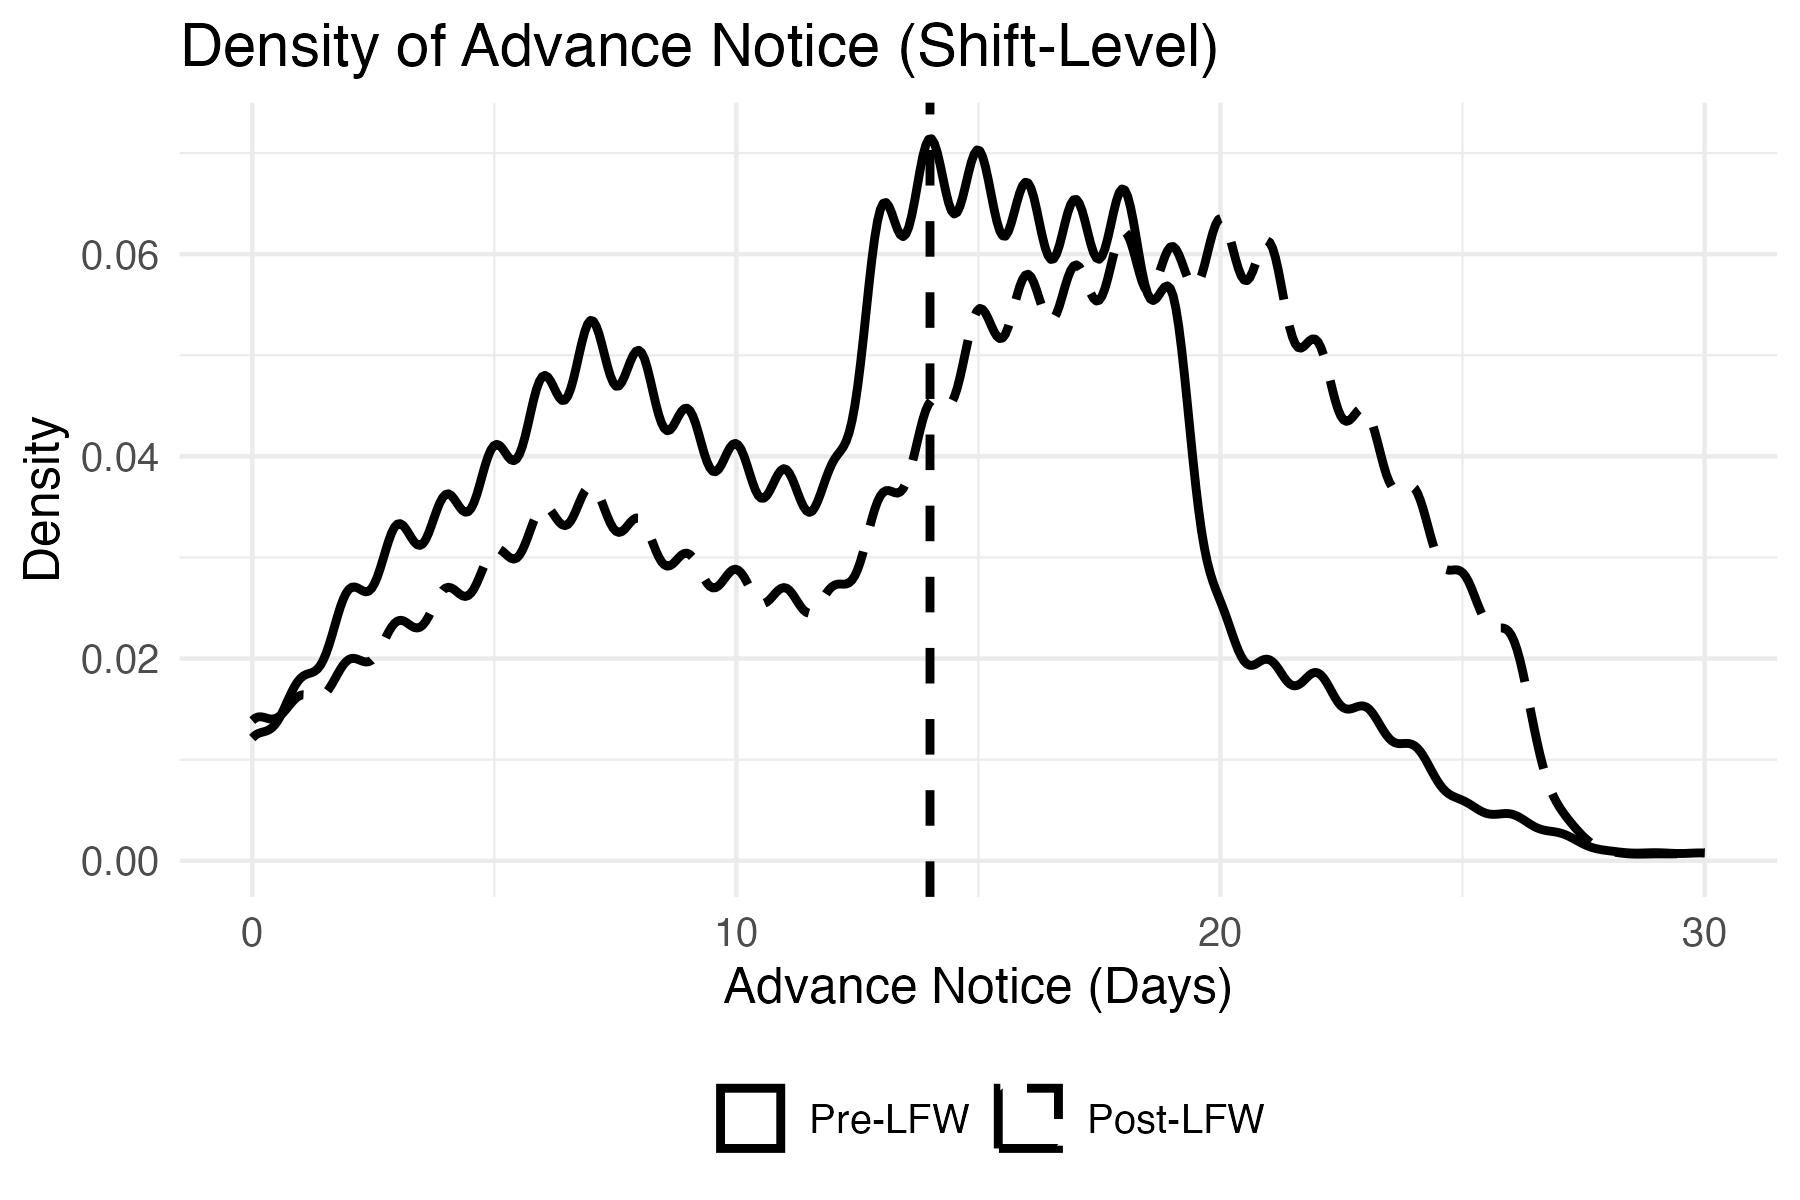
\includegraphics[scale=0.20]{Figures_Revision_2/advance_notice_density_la_pre.jpeg}
%\vspace{-0.0.75cm}
\note{\scriptsize \singlespacing \textit{Notes}: The above figure plots the density of advance notice periods (in days) for shifts in Los Angeles stores before and after the implementation of the LFW. The solid line represents the distribution of advance notice in the pre-LFW period, while the dashed line shows the distribution in the post-LFW period. The vertical dashed line marks the 14-day advance notice threshold for shifts in a given work period.}
\label{f:adv_notice_plot}
\end{figure}
Additionally, we present visual, model-free evidence of how the LFW affected the distribution of advance notice in Figure \ref{f:adv_notice_plot}, which is based on our full sample of more than 100 million shifts. The proportion of shifts with less than 14 days' notice decreased from 49.9\% to 34.8\%—a 15.1 percentage point reduction. However, over one-third of shifts still receive less than the mandated notice after implementation. This persistence of short-notice scheduling indicates that the LFW does not eliminate last-minute changes but rather prices them. Operational needs continue to drive scheduling flexibility through either paid predictability premiums or employee-initiated changes exempt from penalties. While our data cannot separate these two channels, the results demonstrate that firms maintain substantial scheduling flexibility despite the law's requirements.




\paragraph{Event Study Estimates:}
Next, we estimate our event study specification (Equation \ref{eq:model_dynamic}) to assess parallel trends and examine dynamic effects. Panel (a) of Figure \ref{f:event_study_workers} presents these estimates, while Panel (b) shows results for the matched sample discussed in Section \ref{sec:robustness_tests}. Pre-trend coefficients are statistically insignificant at the 5\% level, supporting our parallel trends assumption. We find that the effects materialize gradually, with material increases beginning two months after implementation. This timing aligns with the ordinance's 180-day grace period, during which the city issued only written warnings before full enforcement began in September 2023. Our 22-month post-period provides confidence that these estimates reflect settled responses rather than temporary implementation adjustments.


\begin{figure}[h]
\centering
\begin{subfigure}{.48\textwidth}
  \centering
  \caption*{(a) Full Sample}
  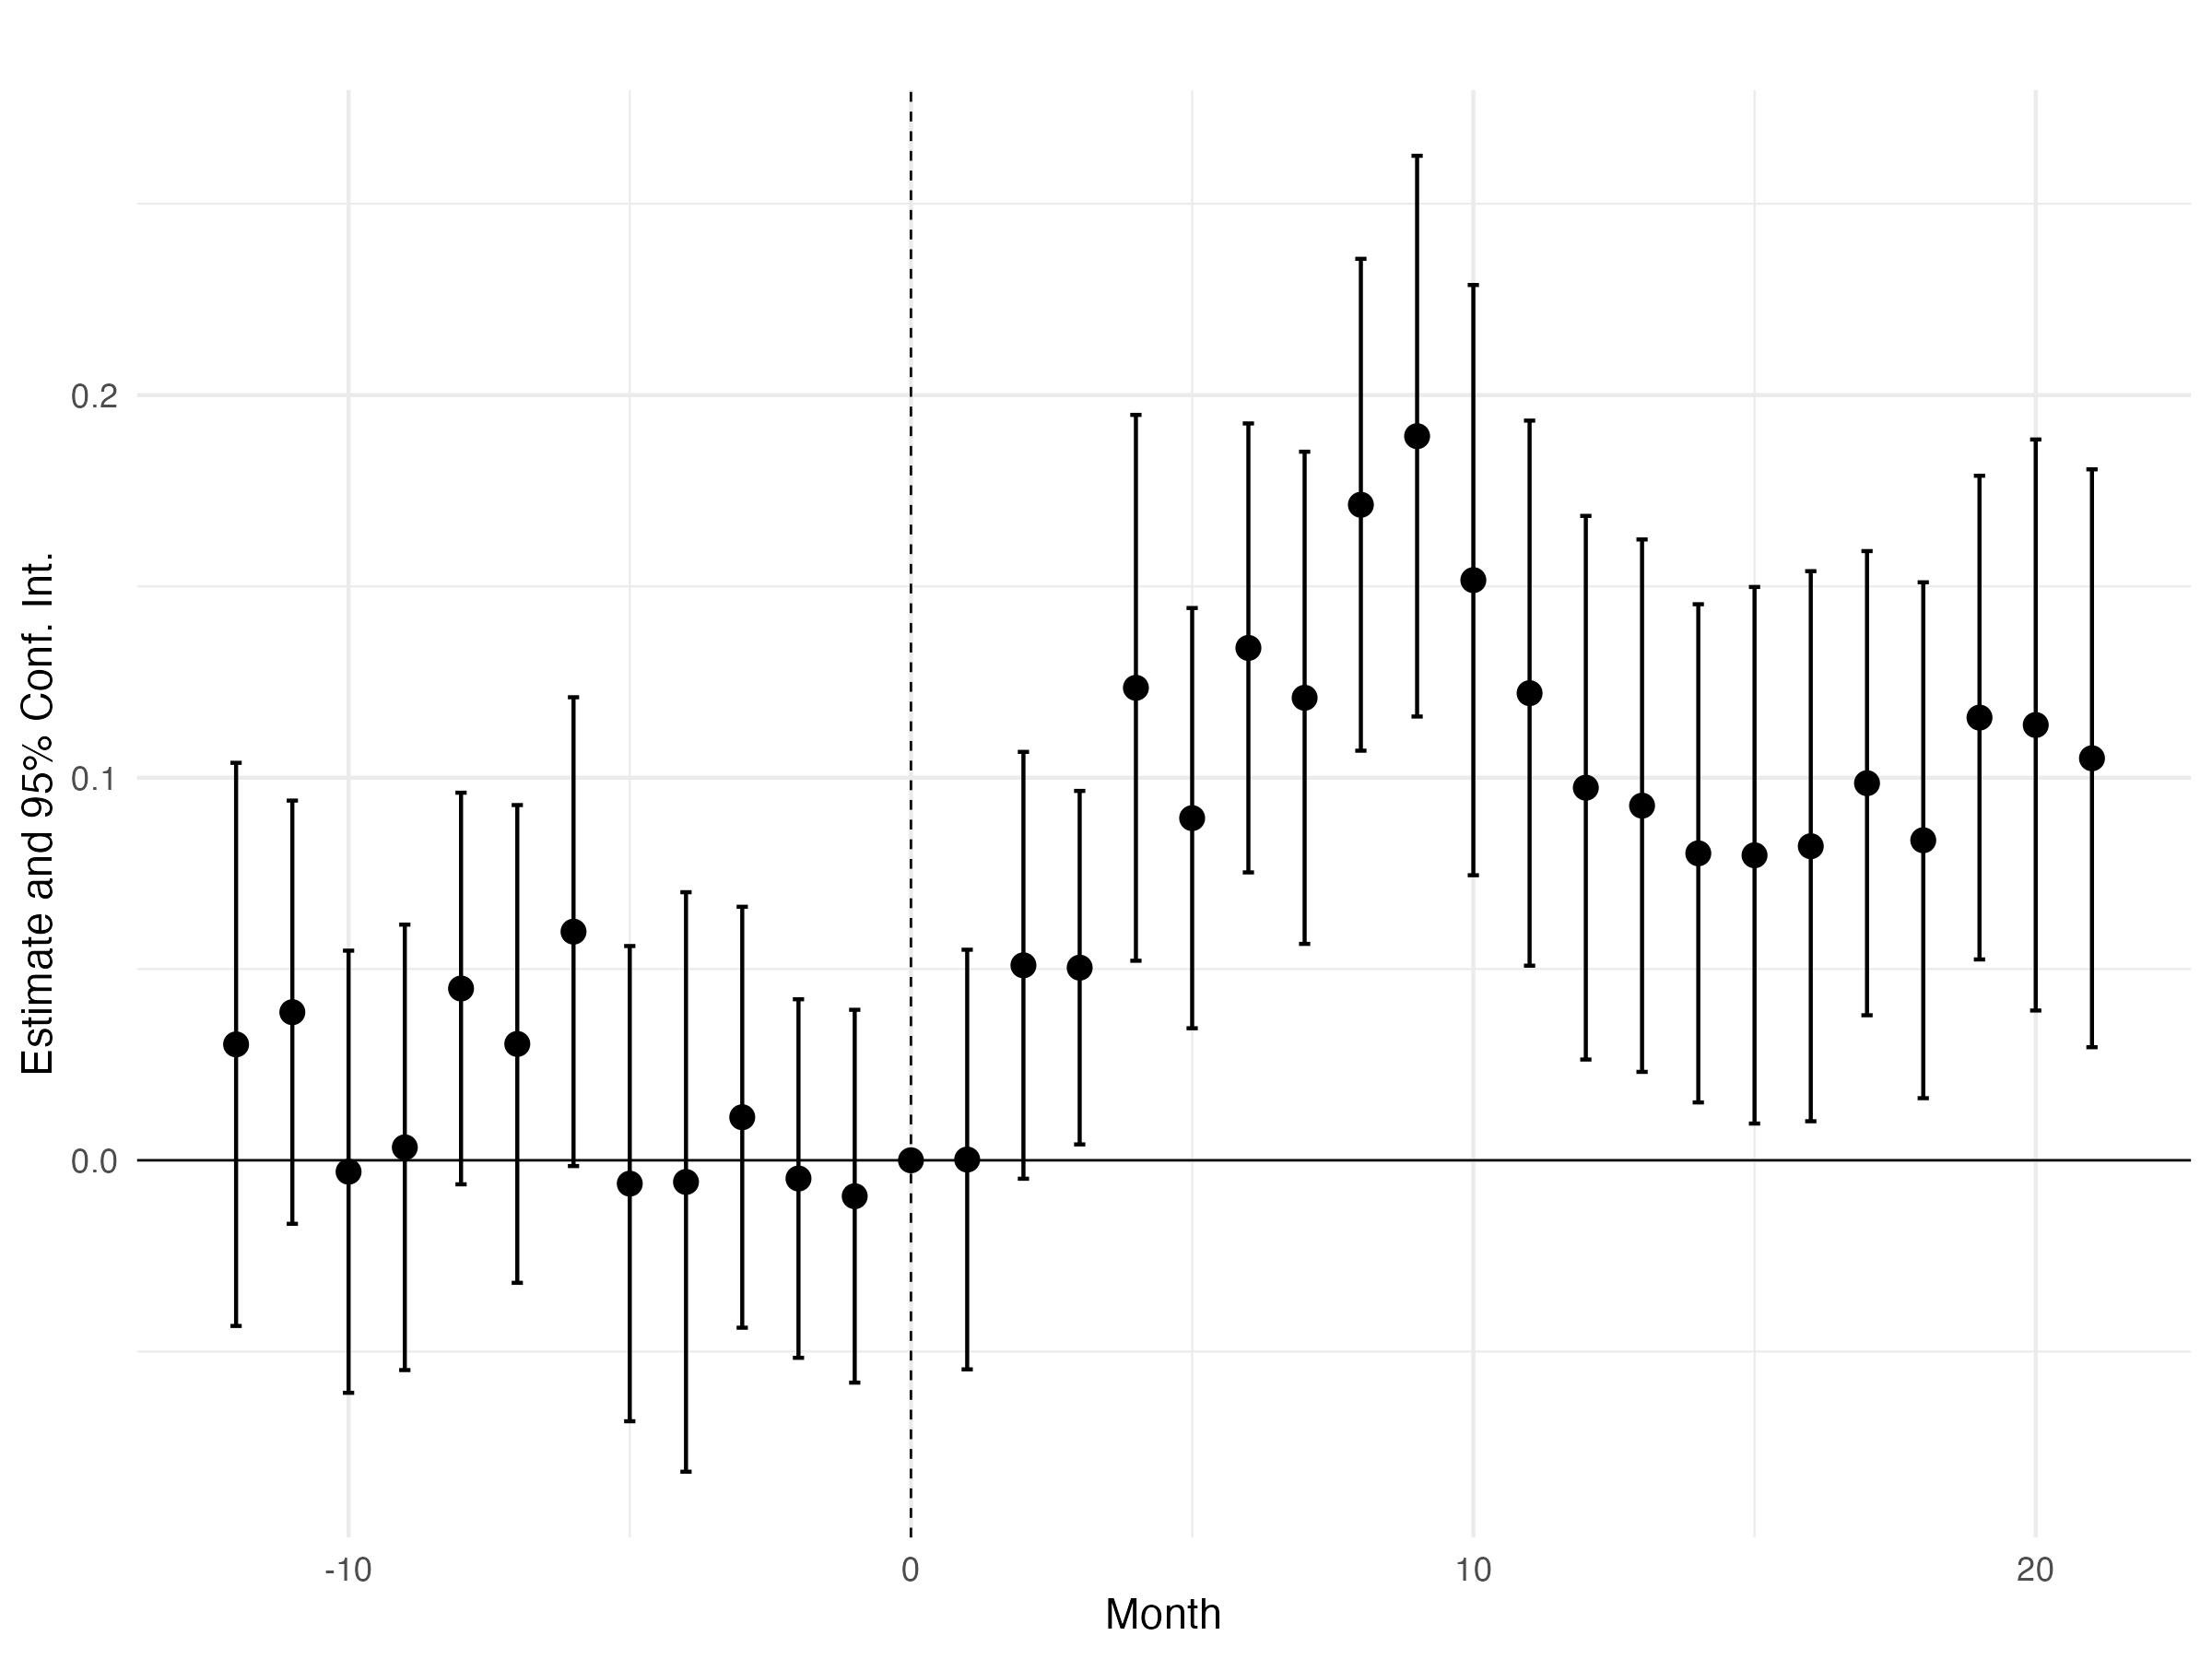
\includegraphics[scale=0.11]{Figures_Revision_2/advance_notice_es_new.jpeg}
  \label{f:event_study_workers_a}
\end{subfigure}%
\begin{subfigure}{.48\textwidth}
  \centering
  \caption*{(b) Matched Sample}
  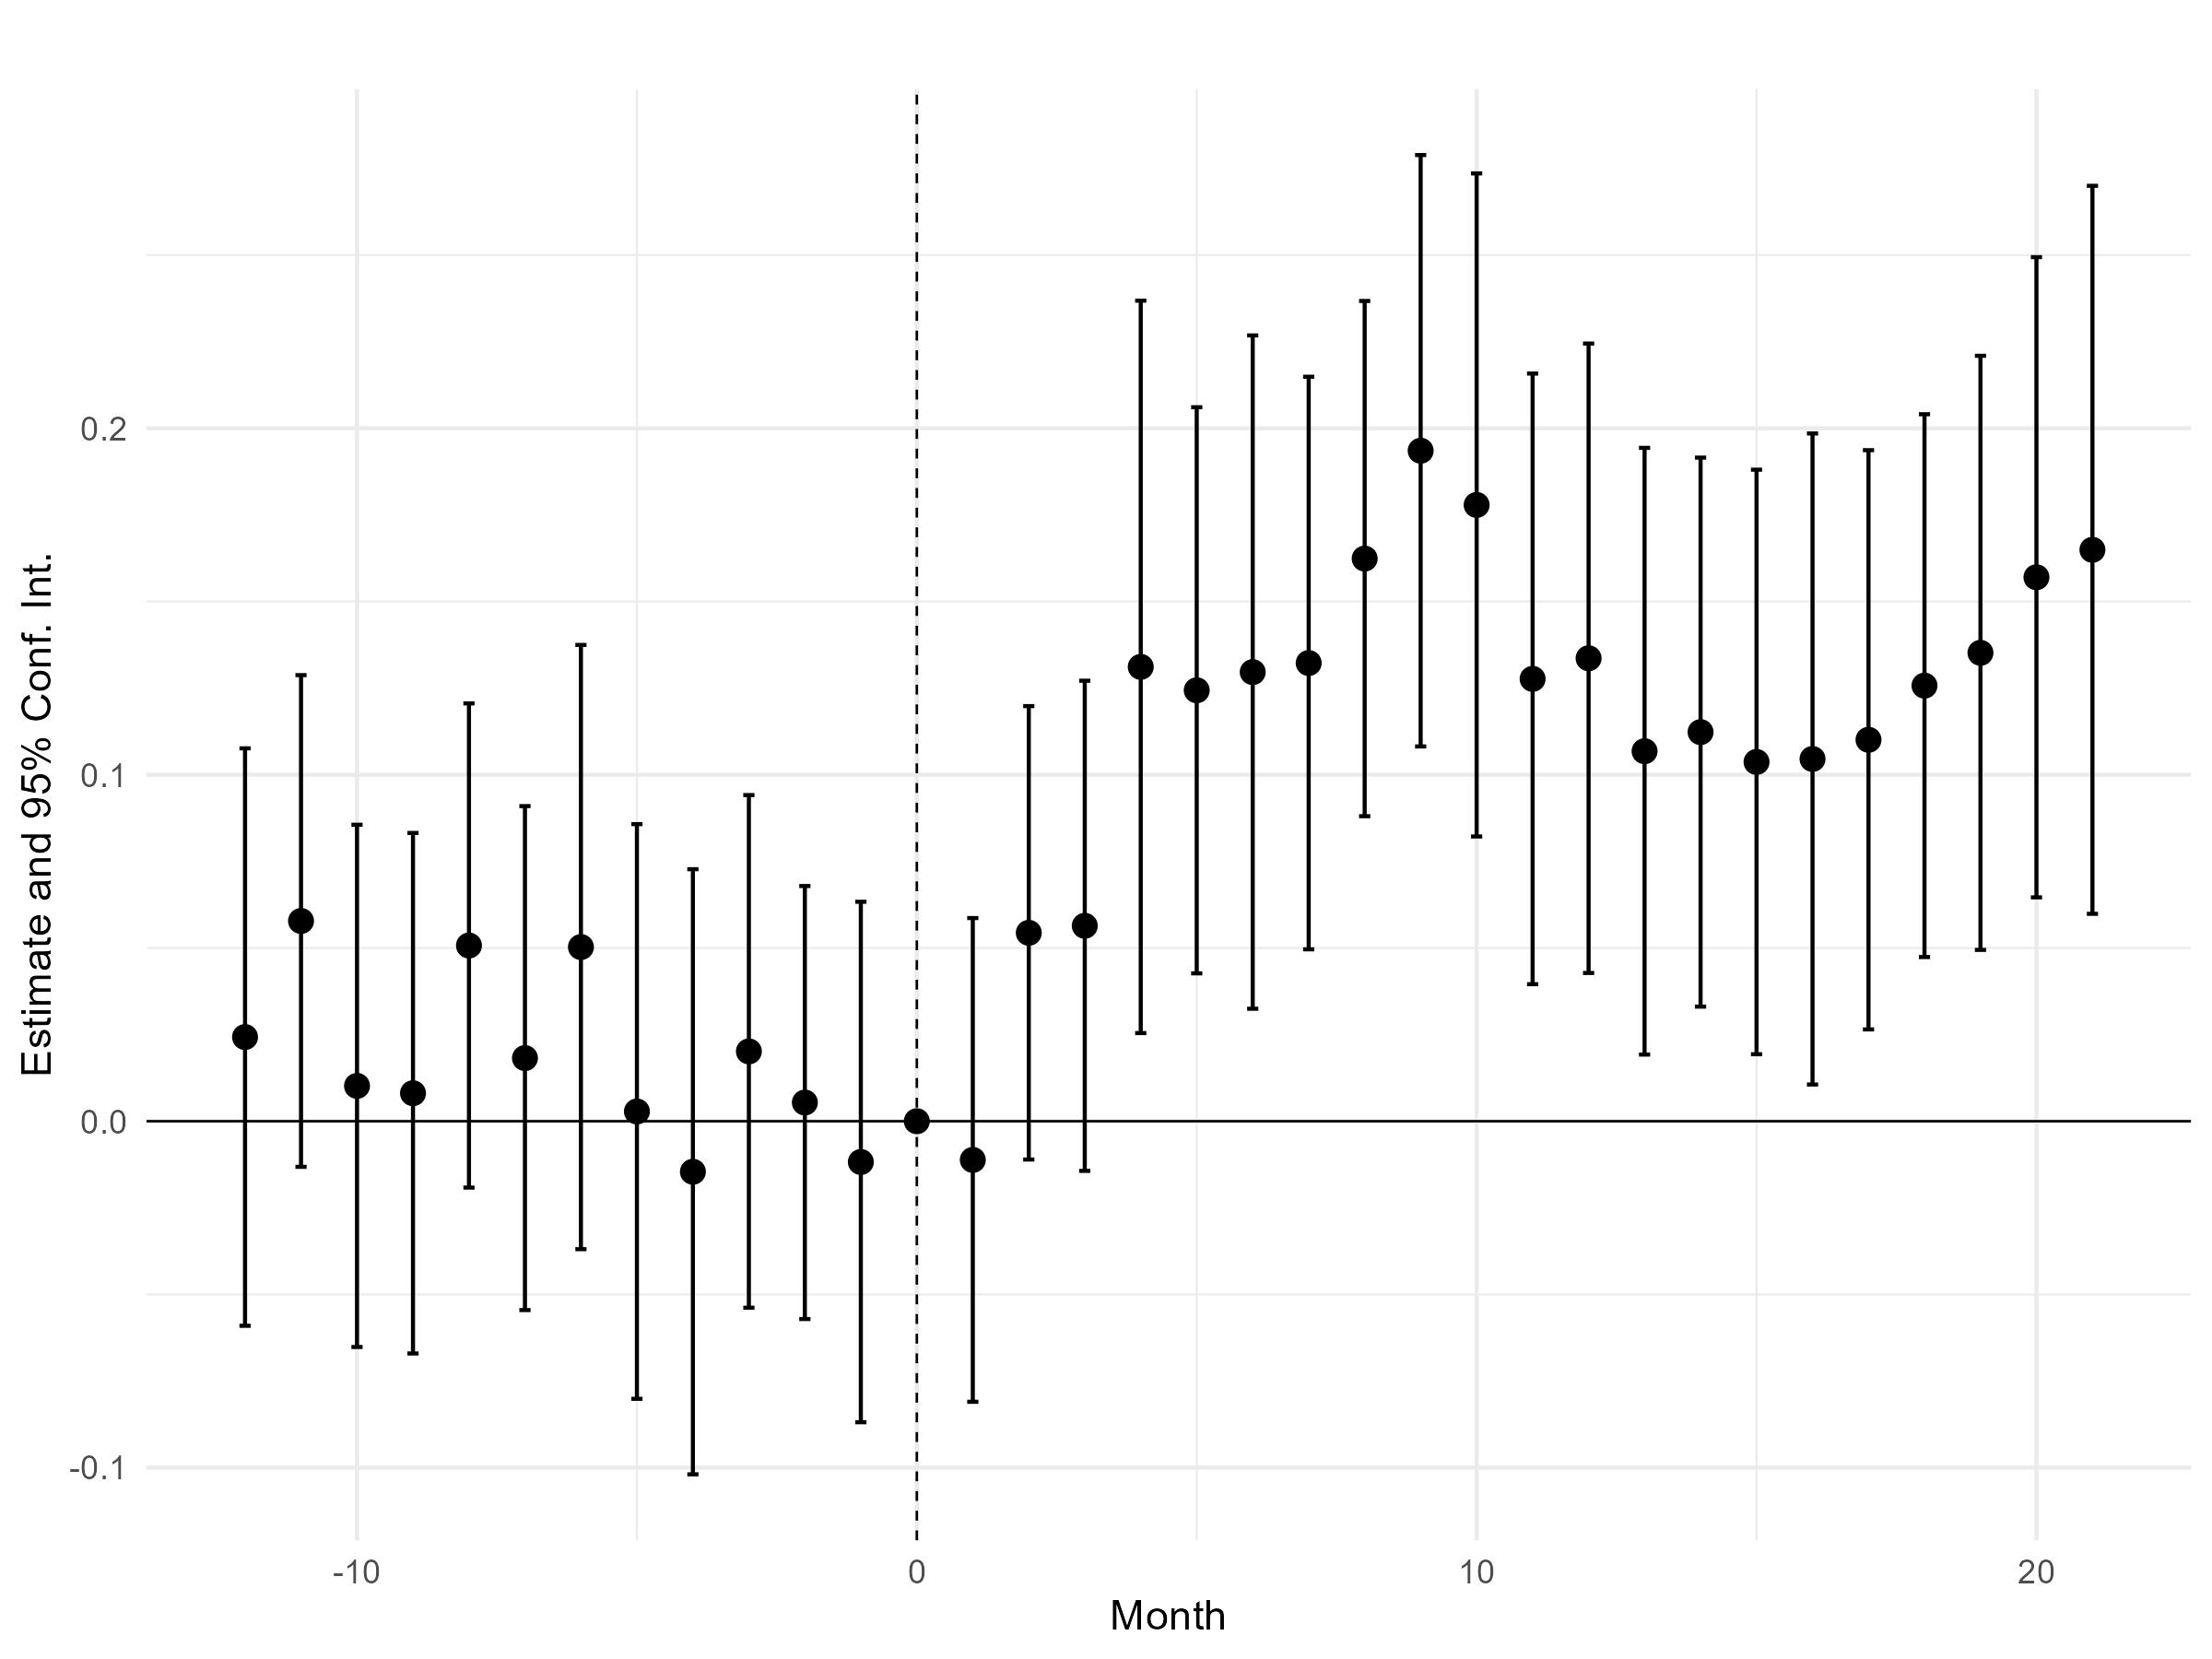
\includegraphics[scale=0.11]{Figures_Revision_2/advance_notice_es_matched_new_v3.jpeg}
  \label{f:event_study_workers_b}
\end{subfigure}
\caption{Event Study Plot for Schedule Predictability}
\vspace{-0.50cm}
\note{\scriptsize \singlespacing \textit{Notes:} The above figure presents event-study coefficients associated with Equation \ref{eq:model_dynamic}. Panel (a) presents the estimates from the full sample, whereas Panel (b) presents estimates from our matched sample (Discussed in Section \ref{sec:robustness_tests}). Each point represents the coefficient associated with $\beta_{k}$, which is the effect of the LFW on the (log) average amount of advance notice in days, which is the average amount of advance notice for all shifts scheduled for the focal worker. Estimates are relative to the focal month of the FWL, which is indicated by the dashed vertical line. All worker-level and store-level control variables are included (See the final column of Table \ref{table:adv_notice}). The bands around estimates are 95\% confidence intervals that are constructed using standard errors that are double clustered at the store and company-year-month levels.}
\label{f:event_study_workers}
\end{figure}

\paragraph{Robustness of Estimates:}
We conduct three robustness tests to ensure our findings are not artifacts of concurrent policies, sample period choices, or multiple hypothesis testing. First, we address the concurrent minimum wage increase (from \$16.04 to \$16.78) implemented in Los Angeles on July 1, 2023. As detailed in Appendix \ref{sec:min_wage_changes}, multiple pieces of evidence indicate our results are driven by the FWL: less than 6\% of workers earned minimum wage (in our wage-observed sample), our pre-period included a similar wage increase with no effects on advance notice, and estimates remain unchanged when excluding minimum wage workers (from our wage-observed sample). We refer the reader to Appendix \ref{sec:min_wage_changes} for full details.

Second, we test sensitivity to alternative analysis windows. While our main specification uses 34 months of data, Table \ref{table:time_windows} examines different temporal boundaries to ensure our results are not artifacts of the chosen time window. Column 1 presents a symmetric 24-month window (12 months pre- and 12 months post-implementation), yielding an estimate of 8.8\%, nearly identical to our main estimate of 8.6\%. Columns 2-4 use asymmetric windows that maintain our full pre-period while extending the post-period to 12, 16, and 18 months, respectively. These specifications produce consistent estimates of 8.8\%, 8.5\%, and 8.5\%, demonstrating that our results are robust to the length of the post-implementation period.

Third, we note that our main finding remains robust to multiple hypothesis testing corrections. With a t-statistic of 4.78 in our preferred specification (Column 4), the treatment effect remains statistically significant at the 5\% level even after applying a Bonferroni correction for up to 2,500 independent hypothesis tests. This level of robustness provides reassurance that our secondary outcome analyses do not undermine the statistical significance of our primary finding. Taken together, these robustness checks reinforce our conclusion that the Los Angeles FWL increased advance notice by approximately 8.5-8.8\% across various specifications.


\paragraph{Heterogeneous Effects (Worker-Level):}
Next, we examine heterogeneous effects across worker characteristics to understand the differential impacts of the LFW. Since we do not observe all characteristics for all workers in our sample (based on the data provided to us by the retailers), we first verify that our main effect is similar when restricting to samples where the characteristic of interest is available. For instance, we observe wages for only 35\% of our worker-month observations. We then estimate heterogeneous effects by augmenting our baseline specification with interactions between the treatment variable and the worker characteristic.

Table \ref{table:adv_notice_het_effects} presents these results. The odd-numbered columns show baseline estimates for each restricted sample, while even-numbered columns add interaction terms to examine heterogeneous effects. Columns 1-6 present results for hourly wages, part-time status, and gender. Columns 7-8 split the sample between non-managerial and managerial workers and examine heterogeneous wage effects within these subsamples. The baseline DiD treatment effects in the odd-numbered columns remain stable across these subsamples, ranging from 8.9 to 11.0 percent increases in advance notice (larger than our baseline estimate of 8.6 percent).\footnote{Note that for wage specifications (Columns 1-2, 7-8), the baseline LA $\times$ Post-LFW coefficient cannot be directly interpreted as it represents the effect for workers with zero wages, which does not exist in our sample.} 

Several patterns emerge when examining heterogeneous effects. Higher wages are associated with smaller policy effects: each dollar increase in hourly wages reduces the effect by 1.2 percentage points (Column 2), though this relationship exists only for non-managerial workers (Column 7) and not for managers (Column 8). This finding runs counter to our initial hypothesis that higher-wage workers would experience greater improvements due to costlier predictability penalties. Instead, the results suggest that lower-wage workers benefited more from the law's requirements. Part-time workers experience 4.2 percentage point smaller increases compared to full-time workers (Column 4), while we find no significant gender differences (Column 6). These results reveal that the law's benefits are concentrated among lower-wage, full-time, non-managerial workers. The finding that part-time workers experience smaller increases aligns with our hypothesis that part-time workers, who may be seeking additional hours, could be more likely to “voluntarily” accept short-notice shifts, thereby exempting employers from penalties due to the law's employee-initiated change provisions.


%% Effect on Store-Labor
\begin{singlespace}
\begin{table}[h]
\caption{Heterogeneous Effects on Schedule Predictability (Worker Characteristics)}

% Created: 2024-12-14 17:17:58.001904
\begingroup
\centering
\scriptsize
\begin{tabular}{lcccccccc}
   \toprule
    & \multicolumn{8}{c}{log(Avg. Adv. Notice)}\\
                                               & (1)           & (2)            & (3)           & (4)           & (5)           & (6)           & (7)            & (8)\\  
   \midrule 
   LA $\times$ Post-LFW                        & 0.110$^{***}$ & 0.243$^{***}$  & 0.089$^{***}$ & 0.105$^{***}$ & 0.092$^{***}$ & 0.089$^{***}$ & 0.263$^{***}$  & -0.094\\   
                                               & (0.029)       & (0.043)        & (0.020)       & (0.021)       & (0.018)       & (0.019)       & (0.046)        & (0.123)\\   
   LA $\times$ Post-LFW $\times$ Hourly Wage   &               & -0.012$^{***}$ &               &               &               &               & -0.014$^{***}$ & 0.003\\   
                                               &               & (0.003)        &               &               &               &               & (0.003)        & (0.004)\\   
   LA $\times$ Post-LFW $\times$ Part-Time     &               &                &               & -0.042$^{**}$ &               &               &                &   \\   
                                               &               &                &               & (0.017)       &               &               &                &   \\   
   LA $\times$ Post-LFW $\times$ Male          &               &                &               &               &               & 0.007         &                &   \\   
                                               &               &                &               &               &               & (0.017)       &                &    
    \\
   Observations                                & 4,041,148     & 4,041,148      & 9,125,224     & 9,125,224     & 9,770,350     & 9,770,350     & 3,656,684      & 381,388\\  
   Adjusted R$^2$                              & 0.719         & 0.719          & 0.712         & 0.712         & 0.577         & 0.577         & 0.722          & 0.711\\  
    \\
   Store FEs                                   & $\checkmark$  & $\checkmark$   & $\checkmark$  & $\checkmark$  & $\checkmark$  & $\checkmark$  & $\checkmark$   & $\checkmark$\\   
   Employee FEs                                & $\checkmark$  & $\checkmark$   & $\checkmark$  & $\checkmark$  & $\checkmark$  & $\checkmark$  & $\checkmark$   & $\checkmark$\\   
   Company-Month FEs                           & $\checkmark$  & $\checkmark$   & $\checkmark$  & $\checkmark$  & $\checkmark$  & $\checkmark$  & $\checkmark$   & $\checkmark$\\   
   \bottomrule
\end{tabular}
\par\endgroup



\note{\scriptsize \textit{Notes: } The estimates above correspond to our heterogeneous effects analyses using difference-in-differences estimates associated with Equation \ref{eq:model} at the worker-month level. The dependent variable is the average amount of advance notice (in days) across shifts. For columns 1-6, odd-numbered columns present baseline estimates (for the sample where the respective worker characteristic is non-missing), and even-numbered columns show the triple difference-in-differences specification. Columns 7-8 split the sample between non-managerial and managerial workers, respectively. All specifications include the full set of fixed effects (worker, store, and company-month) and control variables from Column 4 of Table \ref{table:adv_notice}. Standard errors that are double clustered at the store and company-year-month levels are presented in parentheses. *, **, and *** imply that coefficients are significant at the 10\%, 5\%, and 1\% levels, respectively.}
\label{table:adv_notice_het_effects}
\end{table}
\end{singlespace}





\subsection{Mechanisms For Increased Advance Notice} \label{subsec:adv_notice}
\paragraph{Distributional Effects:}
Earlier, we saw in Figure \ref{f:adv_notice_plot} that the LFW led to a substantial rightward shift in advance notice. The distributional patterns revealed in this figure are critical because a positive average effect in our baseline regression estimates could mask important heterogeneity in how stores adjusted their scheduling practices. For instance, a positive average effect could arise in two distinct ways: stores could shift all scheduling earlier (e.g., moving 2-day notice shifts to 4 days, 4-day notice to 6 days, and so on), or they could increase the number of very short-notice shifts (e.g., 0-2 days) while implementing an even larger increase in long-notice shifts that raises the overall average. This latter possibility would make the interpretation of our average effects more nuanced and would warrant closer investigation of which workers receive short versus long notice shifts for welfare considerations.

To more formally characterize changes to the distribution of advance notice while controlling for fixed and time-varying differences across workers and stores, we estimate a series of regressions using Equation \ref{eq:model}, where the dependent variables are the share of shifts scheduled within specific advance notice ranges (0-1 days, 1-2 days, and so forth up to 26+ days) for each worker-month. Figure \ref{f:adv_notice_distribution} summarizes these estimates. For very short-notice shifts (0-1 day), we find no statistically significant changes. However, statistically significant reductions emerge for shifts scheduled 2-5 days in advance (0.82-0.90 percentage point decreases, based on 95\% confidence intervals). These reductions become larger for shifts scheduled 6-9 days ahead, with decreases of 1.18 and 1.36 percentage points for 6-7 and 8-9 day periods, respectively. The largest reduction occurs in the 12-13 day range (1.56 percentage point decrease), followed by the 14-15 day period (1.51 percentage point decrease).

The effects transition to statistically insignificant changes for shifts scheduled 16-19 days in advance, before showing substantial increases for longer notice periods. The largest increase occurs for shifts scheduled 20-21 days in advance (2.87 percentage points). We also observe statistically significant increases of similar magnitude (approximately 2.15 percentage points) for both 22-23 day notice periods and very long notice periods ($\geq$26 days). These estimates suggest that compliance with the 14-day workweek requirement leads to systematically longer advance notice periods. Because firms must post complete workweeks, shifts scheduled later in the posted week mechanically receive more advance notice than shifts at the start of the week.\footnote{To our knowledge, the "work period" among the retailers in our sample is one week.}



%\newpage 
\begin{figure}[h]
\centering
\caption{Regression Coefficients of Distributional Effects}
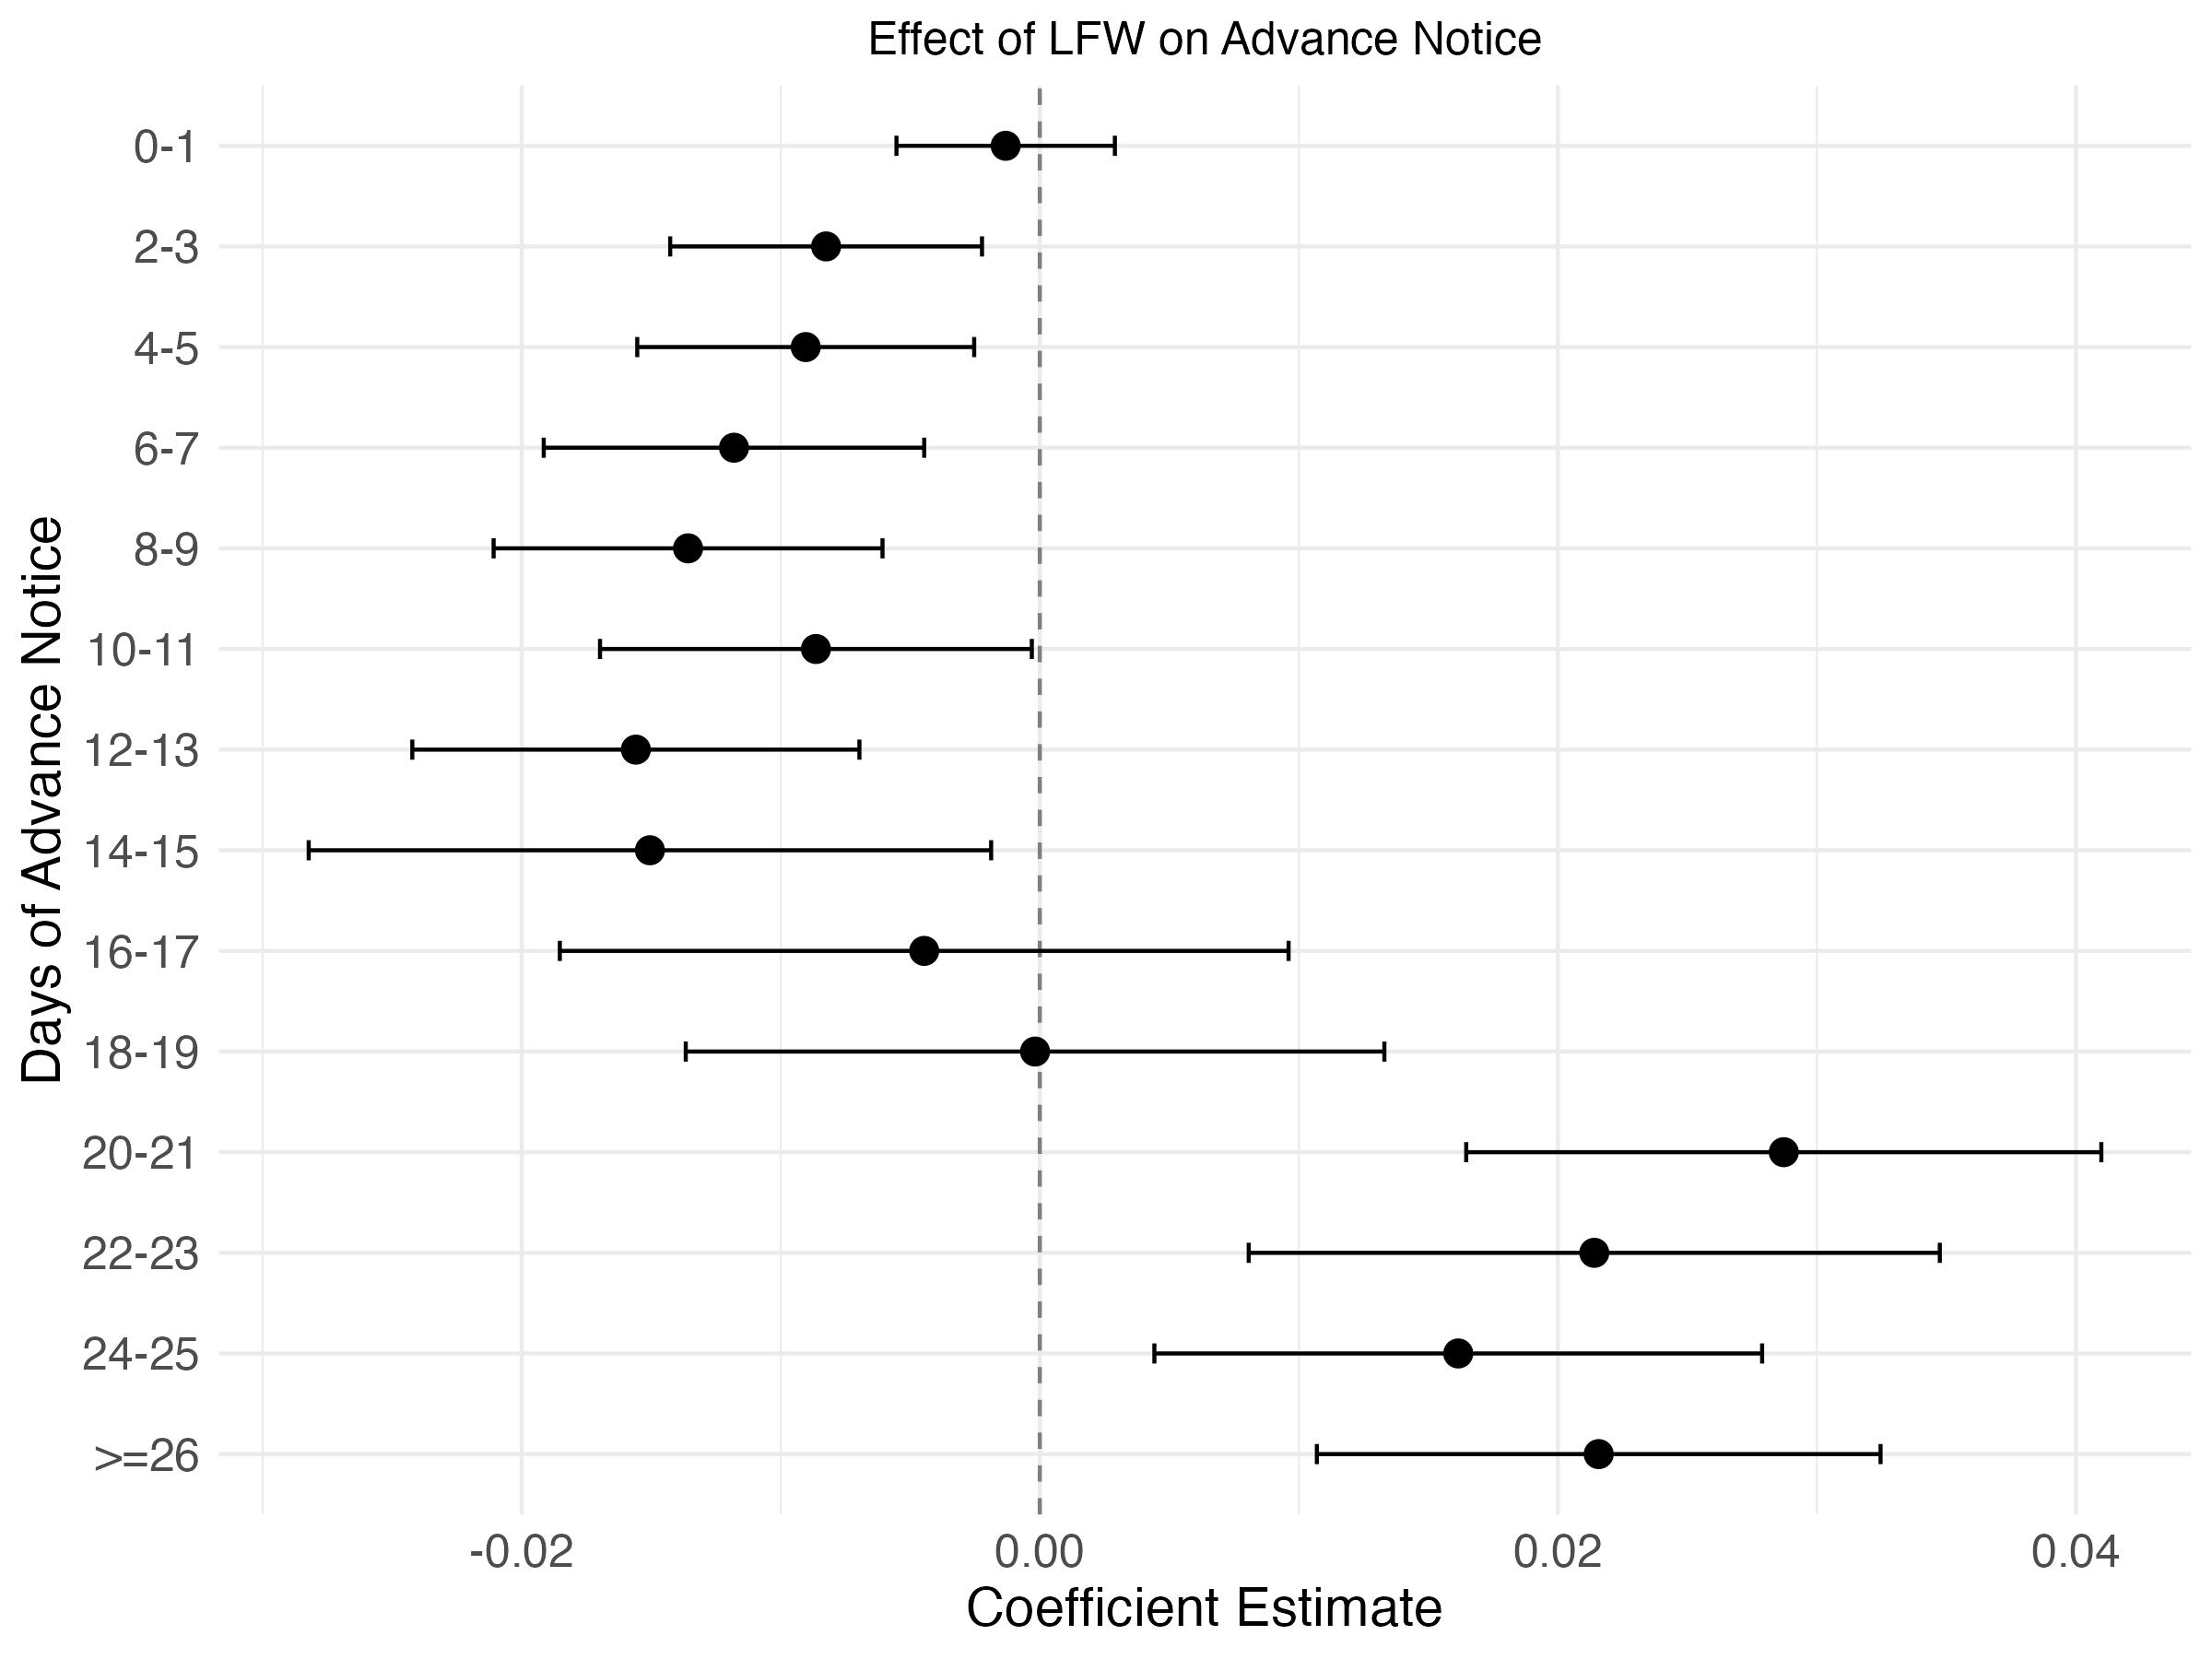
\includegraphics[scale=0.16]{Figures_Revision_2/advance_notice_distr_plot_new.jpeg}
\vspace{-0.50cm}
\note{\scriptsize \singlespacing \textit{Notes: } The above figure plots coefficient estimates measuring how the LFW affected the distribution of advance notice periods at the worker-month level. For each worker-month, we calculate the ratio of shifts that received each length of advance notice (e.g., 0-1 days, 1-2 days) relative to their total shifts that month. Each point represents the estimated impact of the LFW on these ratios. The horizontal bars represent 95\% confidence intervals constructed using standard errors clustered at the store and company-year-month levels. }
\label{f:adv_notice_distribution}
\end{figure}

\paragraph{Effects on Scheduling Actions:}

The aggregate increase in advance notice could mask important differences in how managers adjusted specific types of schedule modifications. Managers could achieve a higher average notice by reducing short-notice shift additions, making fewer last-minute deletions, shifting the entire scheduling process earlier, or some combination of these approaches. Understanding these mechanisms matters for both operational and welfare reasons: different modifications serve distinct purposes (additions meet unexpected demand, deletions avoid excess labor), and workers may have heterogeneous preferences regarding change types (some find additions disruptive to plans, while others find cancellations disruptive to earnings).

We analyze how the LFW affected six distinct scheduling actions at the store-month level: (1) shift additions, (2) duration reductions, (3) duration extensions, (4) timing changes, (5) task modifications, and (6) shift deletions. Figure \ref{f:adv_notice_gen} shows the distribution of each action type across advance notice intervals, normalized by total modifications of that type.

The results reveal consistent patterns across all modification types. Shift additions show significant reductions in short-notice changes from 2-3 days (-1.78 percentage points) through 4-5 days (-1.90 percentage points), with effects diminishing but remaining negative through 12-13 days. The pattern reverses around the 14-day threshold, with the largest increases at 18-19 days (2.59 percentage points) and 20-21 days (2.42 percentage points). Shift deletions show larger adjustments—reductions of 2.61 percentage points at 2-3 days and 2.68 percentage points at 6-7 days—before transitioning to increases peaking at 3.07 percentage points for 20-21 day notice. This pattern particularly matters for worker welfare, as last-minute cancellations disrupt expected earnings.

The four granular adjustments—duration changes and task modifications—exhibit remarkably similar patterns, with reductions of approximately 2.0-2.3 percentage points in the 2-7 day window and increases of 2.7-3.1 percentage points at 18-21 days. Importantly, we find no significant changes in the total frequency of any scheduling action type.\footnote{Regressing total counts of scheduling actions at the store-month level on treatment variables yields no statistically significant coefficients at the 5\% level for any of the six categories.} Overall, this consistency across diverse modification types suggests managers comprehensively reorganized their scheduling processes by making decisions earlier. 



\begin{figure}[!htb]
\centering
\caption{Effects on Schedule Edit Types}
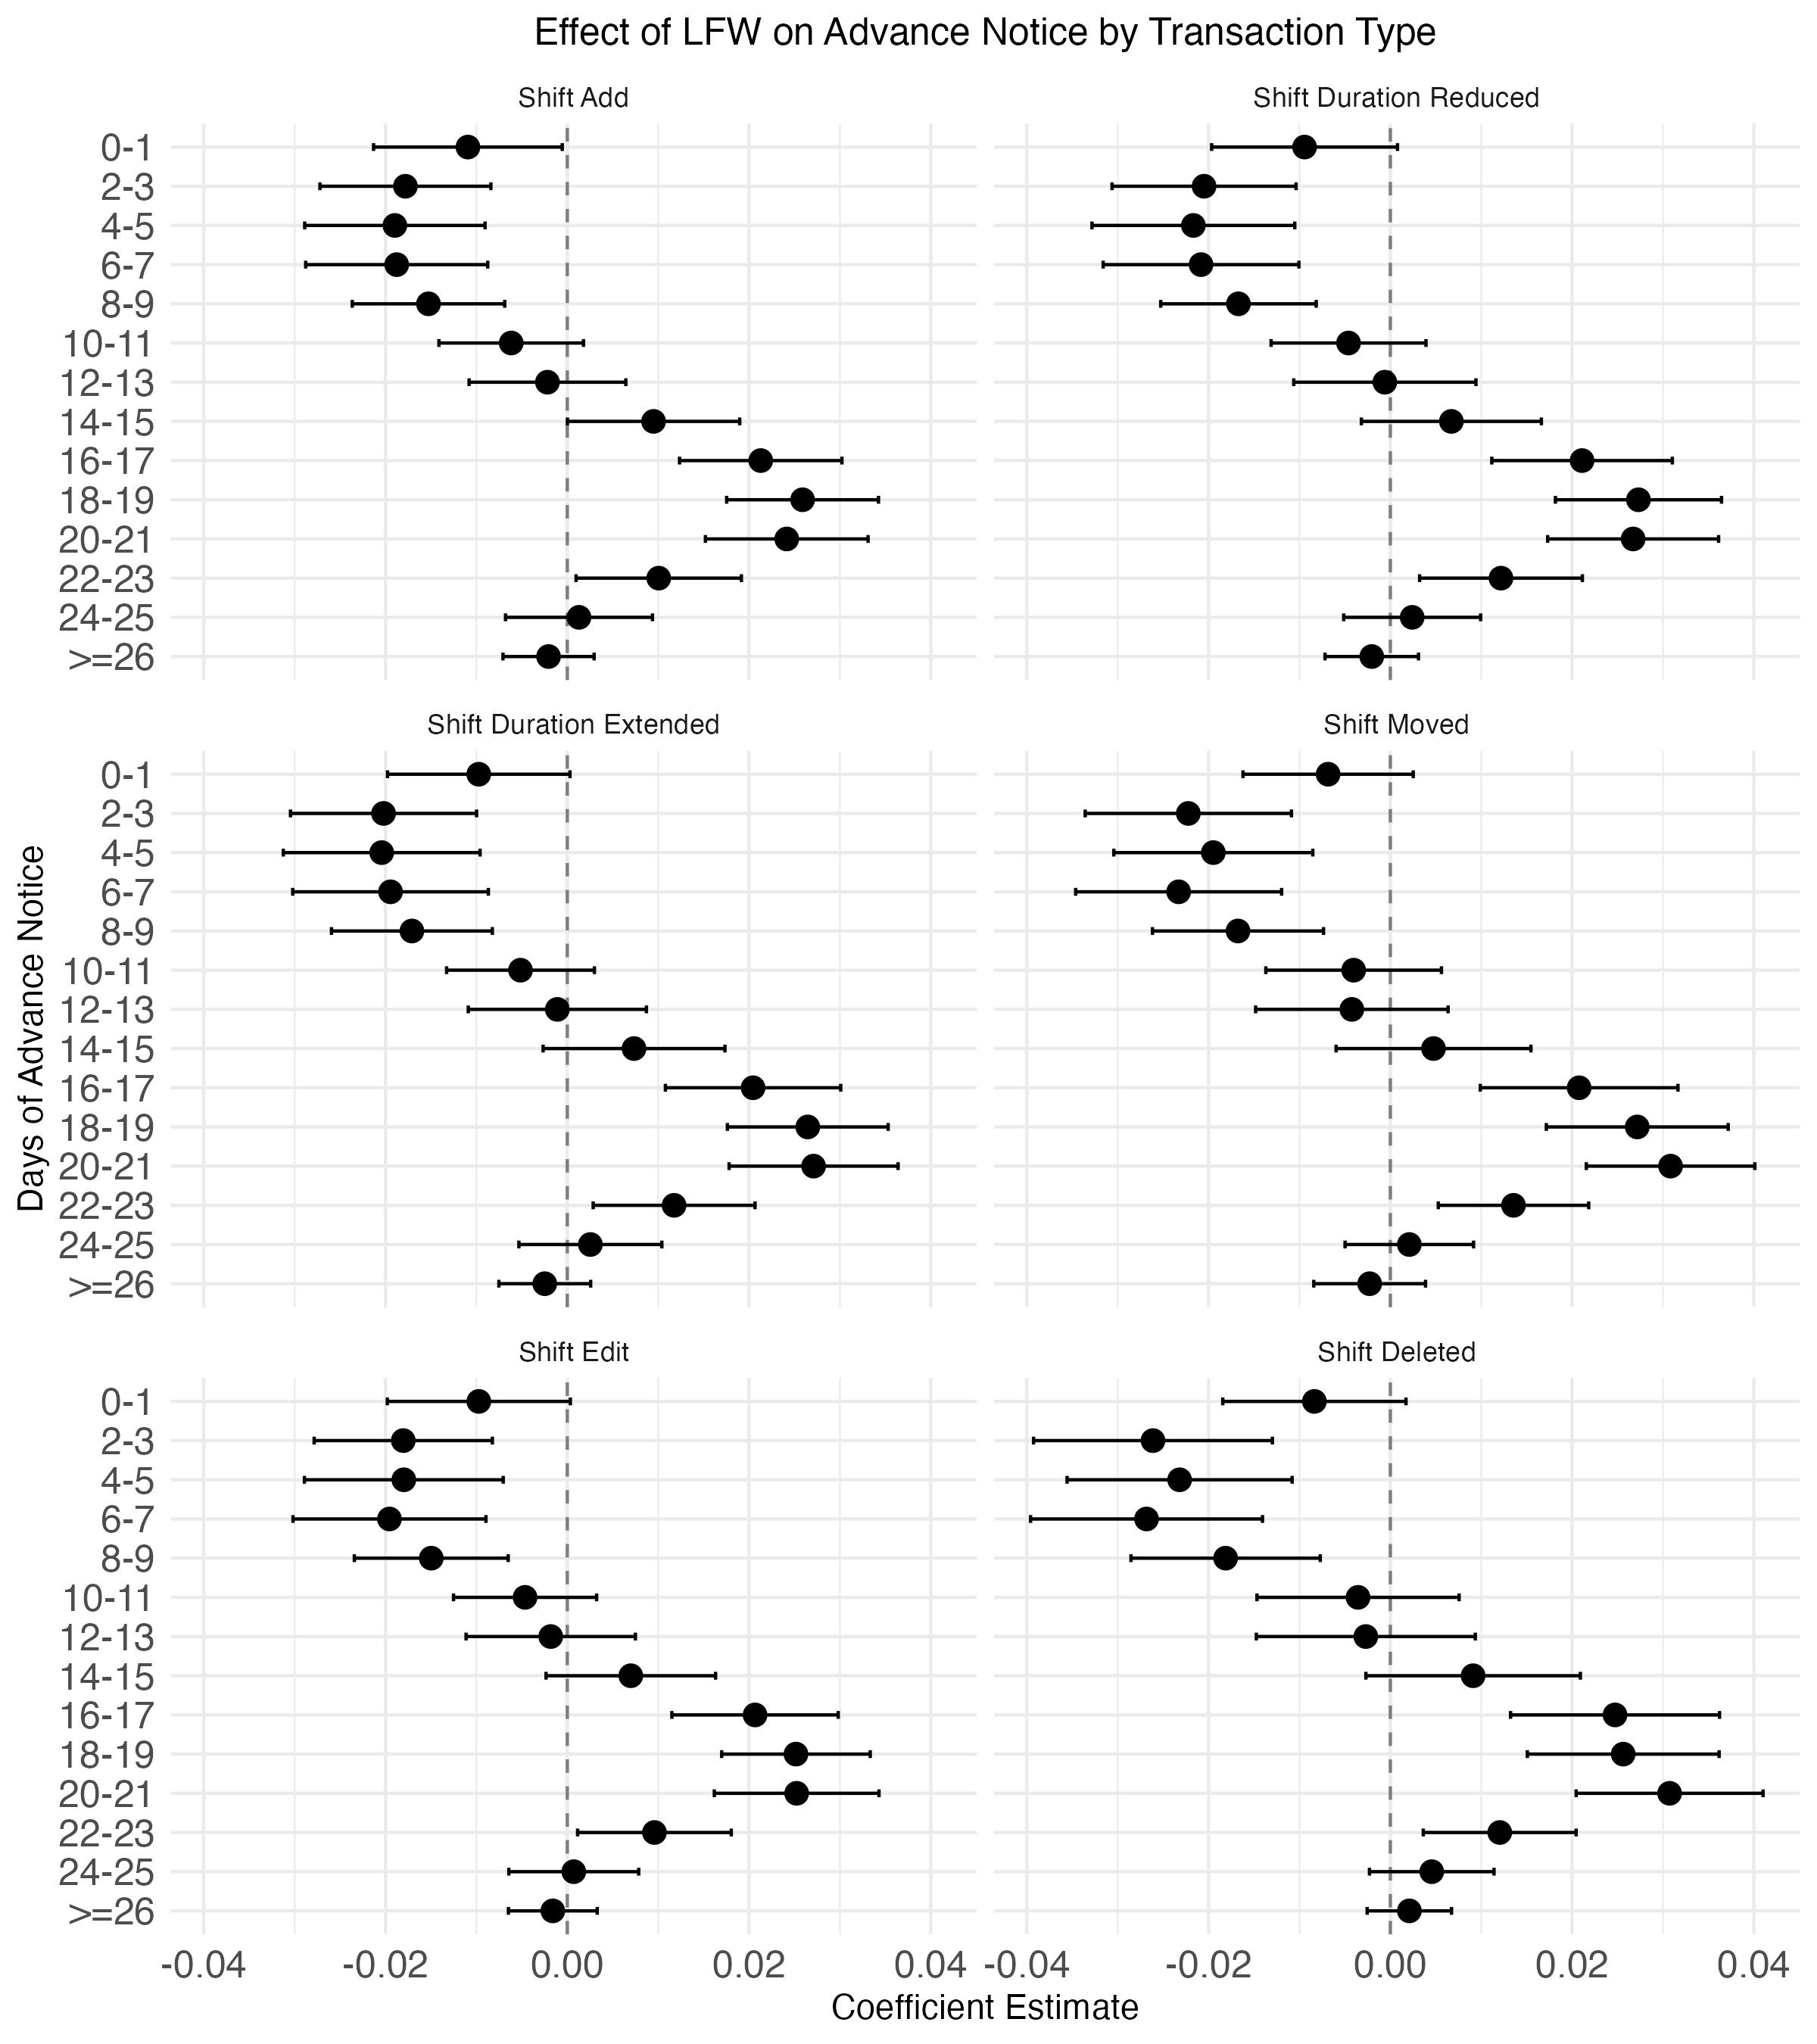
\includegraphics[scale=0.15]{Figures_Revision_2/advance_notice_gen_plot_new_ols.jpeg}
\vspace{-0.50cm}
\note{\scriptsize \singlespacing \textit{Notes: } The above figure plots coefficient estimates measuring how the LFW affected the distribution of advance notice periods. For each store-month, we calculate the ratio of edits that received each length of advance notice (e.g., 0-1 days, 1-2 days) relative to their total edit count that month. Each point represents the estimated impact of the LFW on these ratios. All specifications include store and company-month fixed effects, along with the log-transform of: (1) store demand, (2) store labor supply, and (3) store operating duration in minutes. The horizontal bars represent 95\% confidence intervals constructed using standard errors clustered at the store and company-year-month levels. }
\label{f:adv_notice_gen}
\end{figure}









\subsection{Effects on Schedule Stability} \label{subsec:predict_stability}

While the LFW successfully increased schedule predictability, policymakers frequently promote these laws as improving both predictability \textit{and} stability (see Table \ref{table:tables_for}). However, FWLs contain no provisions that directly incentivize or require schedule stability—they only penalize insufficient advance notice. This regulatory gap raises an important empirical question: can advance notice requirements alone generate the stability improvements that feature prominently in policy advocacy?

We construct four measures normalized by monthly shifts: (1) the standard deviation of shift durations, capturing unpredictable shift lengths that can affect the planning of personal activities and commitments; (2) the standard deviation of weekly hours, as income volatility creates financial instability \citep{Lambert218, schneider2019consequences}; (3) "clopening" shifts (consecutive shifts with less than 10 hours between), which can disrupt sleep and recovery—notably, this is the only stability measure directly addressed by the LFW through its rest-between-shifts provision (Employers must pay employees time and a half for the shift following the insufficient rest period); and (4) start-time inconsistency—shifts beginning more than one hour earlier or later than the same weekday shift in the previous week, which may require workers to readjust their daily routines.




%% Effect on Store-Labor
\begin{singlespace}
\begin{table}[h]
\caption{Effects on Schedule Stability}

% Created: 2025-02-01 15:57:33.407693
\begingroup
\centering
\scriptsize
\begin{tabular}{lcccc}
   \toprule
                         & Shift Duration Variability. & Weekly Hours Variability & Clopening Shifts      &  Unstable Start Times Shifts\\   
                         & (1)            & (2)             & (3)            & (4)\\  
   \midrule 
   LA $\times$ Post-LFW  & -0.118         & -0.007          & -0.002$^{***}$ & -0.003\\   
                         & (0.096)        & (0.005)         & (0.001)        & (0.003)\\   
    \\
   Observations          & 11,670,999     & 11,670,999      & 11,670,999     & 11,670,999\\  
   Adjusted R$^2$        & 0.148          & 0.143           & 0.390          & 0.565\\  
    \\
   Store FEs             & $\checkmark$   & $\checkmark$    & $\checkmark$   & $\checkmark$\\   
   Employee FEs          & $\checkmark$   & $\checkmark$    & $\checkmark$   & $\checkmark$\\   
   Company-Month FEs     & $\checkmark$   & $\checkmark$    & $\checkmark$   & $\checkmark$\\   
   \bottomrule
\end{tabular}
\par\endgroup



\note{\textit{Notes: } \scriptsize The estimates above correspond to our difference-in-differences estimates associated with Equation \ref{eq:model}. The dependent variables measure different aspects of schedule stability at the worker-month level: Column (1) is the standard deviation of shift durations normalized by total shifts, Column (2) is the standard deviation of weekly hours normalized by total shifts, Column (3) is the share of consecutive shifts with less than 10 hours of rest between them (``clopening'' shifts), and Column (4) is the share of shifts that start more than one hour earlier or later than the same day-of-week shift in the previous week (conditional on working both weeks). All specifications include the full set of fixed effects (worker, store, and company-month) and control variables from Column 4 of Table \ref{table:adv_notice}. Standard errors that are double clustered at the store and company-year-month levels are presented in parentheses. *, **, and *** imply that coefficients are significant at the 10\%, 5\%, and 1\% levels, respectively.}
\label{table:stab_regs}
\end{table}
\end{singlespace}


Table \ref{table:stab_regs} reveals that advance notice requirements had minimal spillover effects on schedule stability. We find only one statistically significant effect: a 0.002 reduction in the share of clopening shifts. However, this effect is economically negligible—clopening shifts were already rare in our sample with a mean of approximately 0.005, affecting less than 0.5\% of all shifts. The remaining stability measures—shift duration variability, weekly hours consistency, and start-time regularity—show no significant changes. These null results are precisely estimated, allowing us to rule out economically meaningful improvements in schedule stability. This finding provides important insight for policymakers: advance notice requirements alone do not appear to generate the stability improvements often promised in policy advocacy. Our evidence suggests that if stability is a primary goal, it likely requires explicit regulatory provisions rather than relying on indirect effects from predictability mandates.

Finally, we examine whether schedule stability improvements differ by employment type, focusing on part-time workers who are particularly vulnerable to unstable schedules. Given that part-time workers already experienced smaller gains in advance notice (4.2 percentage points less than full-time workers), we test whether firms might similarly preserve stability for full-time workers while maintaining or even increasing instability for part-time workers—potentially using part-time workers as a buffer to absorb scheduling variability. Running a triple difference-in-differences specification interacting treatment with part-time status, we find that the coefficients are small and statistically insignificant across all four stability measures. These null effects are precisely estimated, with coefficients very close to zero, indicating that part-time workers experienced no differential improvements in schedule stability compared to full-time workers, though both groups saw minimal stability gains overall.


Overall, the disconnect between policy rhetoric and actual effects highlights a fundamental limitation of the penalty-based approach. Without explicit incentives for consistency, firms rationally maintain scheduling variability to preserve operational flexibility while complying with advance notice requirements. A worker might receive 14 days' notice of a schedule that varies wildly from week to week, fully satisfying the law while experiencing no improvement in the stability that policymakers promise. This finding challenges a core assumption underlying FWL advocacy—that predictability and stability naturally go hand in hand. Our evidence demonstrates they do not. Policymakers aiming to deliver the comprehensive scheduling improvements they promise to workers must move beyond the current regulatory framework. They need to include explicit stability provisions, rather than assuming such benefits will emerge indirectly from advance notice requirements alone.



\section{Main Results: Effects on Worker and Store Outcomes}

Having established the LFW's success in improving schedule predictability, we now address a critical question in the policy debate: Did these benefits for workers come at the cost of the negative unintended consequences frequently cited by critics (see Table \ref{table:tables_against})? We investigate these potential unintended consequences empirically. 


\begin{singlespace}
\begin{table}[h]
\caption{Effects on Worker Outcomes}

% Created: 2024-12-29 16:46:38.853864
\begingroup
\centering
\scriptsize
\begin{tabular}{lccc}
   \toprule
                         & log(Worker Mins.)    & log(Worker Shifts)   & Approved Availability Change\\  
                         & (1)           & (2)           & (3)\\  
   \midrule 
   LA $\times$ Post-LFW  & 0.008         & 0.002         & 0.024\\   
                         & (0.011)       & (0.010)       & (0.035)\\   
    \\
   Observations          & 11,670,999    & 11,670,999    & 1,282,016\\  
   Adjusted R$^2$        & 0.621         & 0.605         & 0.134\\  
    \\
   Store FEs             & $\checkmark$  & $\checkmark$  & $\checkmark$\\   
   Employee FEs          & $\checkmark$  & $\checkmark$  & $\checkmark$ \\  
   Company-Month FEs     & $\checkmark$  & $\checkmark$  & $\checkmark$\\   
   \bottomrule
\end{tabular}
\par\endgroup






\note{\textit{Notes: } \scriptsize The estimates above correspond to our difference-in-differences estimates associated with Equation \ref{eq:model}. The dependent variables log(Mins.) and log(Shifts) are the log of total scheduled labor minutes and scheduled shifts, respectively.
The first two specifications include the full set of fixed effects (worker, store, and company-month) and control variables from Column 4 of Table \ref{table:adv_notice}. Standard errors that are double clustered at the store and company-year-month levels are presented in parentheses. *, **, and *** imply that coefficients are significant at the 10\%, 5\%, and 1\% levels, respectively.}
\label{table:worker_level}
\end{table}
\end{singlespace}

\subsection{Worker-Level Outcomes} \label{subsec:scheduled_labor}

We examine whether increased schedule predictability came at the cost of reduced work opportunities and scheduling flexibility for employees. Specifically, we analyze changes in scheduled hours and workers' ability to modify their own schedules in response to personal needs.

\paragraph{Total Shifts and Scheduled Minutes:} As hypothesized in Section \ref{sec:hyp}, the LFW's effect on scheduled labor is theoretically ambiguous due to competing forces. The law creates asymmetric penalties: employers pay one hour of regular pay for adding shifts but half wages for canceled shifts, creating different incentives for upward versus downward adjustments. Managers facing this penalty structure might adopt conservative baseline schedules to avoid costly additions when demand spikes. Yet they also face penalties for reductions, which could potentially lead to higher scheduled hours when they overestimate demand. Additionally, any reduction in store operating hours (which we test separately) would mechanically reduce available work hours for employees. However, Columns (1) and (2) of Table \ref{table:worker_level} show no evidence of changes in either direction, with statistically insignificant effects on both total scheduled minutes (0.8\%) and number of shifts (0.2\%). These precise null effects suggest that employers neither systematically reduced hours to avoid penalties nor increased them due to cancellation costs—inconsistent with industry predictions that "98\% are likely to schedule fewer workers per shift" (Table \ref{table:tables_against}).


\paragraph{Availability Change Requests:} As hypothesized in Section \ref{sec:hyp}, the LFW could inadvertently reduce workers' control over their own schedules. When workers request changes in availability—for education, family care, or other needs—managers may need to modify multiple weeks of already-posted schedules, potentially triggering predictability pay for affected coworkers. Combined with the good-faith estimate requirement that creates implicit schedule commitments, we expected managers might deny availability changes they would have previously approved—a concerning outcome since workers value schedule control for managing personal responsibilities \citep{kelly2011changing,harknett2022who,mas2017valuing}. However, analyzing over 1.2 million availability change requests, Column (3) of Table \ref{table:worker_level} shows no statistically significant change in approval rates, with a precise null effect of 2.4 percentage points. This finding contradicts our hypothesis, suggesting that employers developed effective strategies for managing longer-term schedule changes without compromising worker flexibility. The preservation of availability change flexibility is particularly important given that the law aimed to protect workers from employer-driven unpredictability, not to constrain workers' own scheduling agency.

\subsection{Store-Level Outcomes}

Critics also argue that FWLs could fundamentally alter store-level operations and workforce management. Specifically, stores may reduce operating hours, shift toward part-time employment to maintain scheduling flexibility, or face an increased managerial burden in coordinating labor schedules. 



\paragraph{Labor Composition (Part-Time versus Full-Time):} As hypothesized in Section \ref{sec:hyp}, firms may shift toward part-time employment to maintain scheduling flexibility while avoiding penalties. Part-time workers often request additional hours and typically lack benefits, potentially making them more likely to accept ``voluntary'' short-notice shifts that exempt employers from predictability premiums \citep{kalleberg2009precarious,lambert_2008}. Our earlier finding that part-time workers experienced 4.2 percentage point smaller increases in advance notice than full-time workers (Table \ref{table:adv_notice_het_effects}) supports this mechanism—these workers already serve as flexible capacity. Since part-time workers also lack costly benefits, stores may find it economically advantageous to employ more part-time workers and pay occasional scheduling penalties rather than incur the ongoing benefit costs of full-time workers. A larger pool of part-time workers would also expand options for ``voluntary'' schedule changes exempt from penalties. However, Table \ref{table:store_level} shows no evidence of such strategic adjustment. The estimated effects on both the part-time labor ratio (0.4 percentage points) and part-time shift ratio (0.5 percentage points) are small and statistically insignificant, contradicting our hypothesis that stores would systematically alter their workforce composition to circumvent the law's requirements.


\paragraph{Operating Days and Duration:} Critics argue that when schedule adjustments become more costly due to advance notice requirements and penalties, stores may reduce their operating hours or days to minimize exposure to these costs. The logic is that stores may curtail operations during typically volatile periods, such as early mornings or late evenings, when customer demand is less predictable and may require last-minute staffing adjustments. Without the flexibility to call in workers on short notice or ask them to stay longer without incurring penalties, stores may find it optimal to simply close during these hours. However, we find no evidence of such operational changes. The estimated effect on log operating minutes is small (0.4\%) and statistically insignificant, while the impact on operating days in levels is similarly negligible and insignificant. These results suggest that stores maintained their normal operating patterns rather than curtailing operations in response to the scheduling requirements.


\begin{singlespace}
\begin{table}[h]
\caption{Effects on Store Outcomes}
% Created: 2025-01-12 16:54:34.847264
\begingroup
\centering
\scriptsize
\begin{tabular}{lcccccc}
   \toprule
                         & PT Mins. Ratio & PT Shifts Ratio & log(Store Op. Mins) & Op. Days      & Hires         & Turnover\\    
                         & (1)            & (2)             & (3)                 & (4)           & (5)           & (6)\\  
   \midrule 
   LA $\times$ Post-LFW  & 0.004          & 0.005           & 0.004               & -0.003        & -0.008        & 0.002\\   
                         & (0.009)        & (0.009)         & (0.003)             & (0.011)       & (0.070)       & (0.050)\\   
    \\
   Observations          & 654,749        & 654,749         & 654,749             & 654,749       & 654,749       & 654,749\\  
   Adjusted R$^2$        & 0.811          & 0.849           & 0.983               & 0.995         & 0.366         & 0.320\\  
    \\
   Store FEs             & $\checkmark$   & $\checkmark$    & $\checkmark$        & $\checkmark$  & $\checkmark$  & $\checkmark$\\   
   Company-Month FEs     & $\checkmark$   & $\checkmark$    & $\checkmark$        & $\checkmark$  & $\checkmark$  & $\checkmark$\\   
   \bottomrule
\end{tabular}
\par\endgroup
\note{\textit{Notes: } \scriptsize The estimates above correspond to our difference-in-differences estimates associated with Equation \ref{eq:model}.
PT Mins. Ratio is the ratio of part-time scheduled labor minutes to total labor minutes. PT Shifts Ratio is the ratio of shifts assigned to part-time employees to total shifts. Store Op. Mins is the total operating duration in minutes. Op. Days is the total number of operating calendar days. Hires is the total number of new hires. Turnover is the total number of employee separations. All dependent variables are defined at the store-month level. In addition to the fixed effects described above, all regressions include the following store-level control variables (except where the control is the dependent variable of interest): total operating days, total operating duration in minutes, total edits, and the demand forecast. All control variables are log-transformed. Standard errors that are double clustered at the store and company-year-month levels are presented in parentheses. *, **, and *** imply that coefficients are significant at the 10\%, 5\%, and 1\% levels, respectively.}
\label{table:store_level}
\end{table}
\end{singlespace}

\paragraph{Employee Hiring and Turnover:} The LFW could affect employment flows through several channels. Stores may become more cautious about hiring since they must provide good-faith estimates of expected hours and schedules to new employees, potentially creating implicit minimum hour guarantees. On the worker side, improved schedule predictability may reduce turnover by decreasing work-life conflicts. Our estimates for both hiring and turnover are statistically insignificant with large standard errors. The wide confidence intervals reflect substantial month-to-month variation in employment flows, making it difficult to precisely estimate these effects. 




\section{Robustness Tests} \label{sec:robustness_tests}

We conclude the paper with several robustness tests that address potential concerns about sample composition and differential trends across worker and store characteristics.

\subsection{Worker-Level Matching}

First, we assess the robustness of our main results using matched samples to address concerns about differential post-treatment shocks affecting specific employee groups. That is, while our difference-in-differences design controls for time-invariant differences between treatment and control stores, labor market conditions or company policies may evolve differently for workers with different characteristics. By creating more comparable treatment and control groups, this matching approach may also lend additional credibility to our parallel trends assumption.   However, this matching approach comes with a tradeoff: We lose observations because not all employee characteristics are available across all companies in our data. For companies that maintain these records, we observe the complete set of characteristics for all their employees.

Our matching methodology proceeds as follows. We first calculate pre-treatment worker-level variables (average wages, sum of total shifts, and sum of minutes worked) and store-level averages (workload minutes, labor supply, store scheduled labor minutes, store operating minutes, and managerial edits). We then implement nearest-neighbor matching with a probit distance metric that exactly matches workers on part-time status, managerial status, and company affiliation. Within these strata, we find the closest matches based on the pre-treatment worker and store-level variables, as well as Census zip-code-level characteristics, including retail employment share and log per capita income. This approach ensures we compare workers who were similar in their individual work patterns and who worked in stores with similar operational patterns and local economic environments before the LFW was implemented.

Table \ref{table:worker_summary_wide_matched} presents the covariate balance for our matched sample, demonstrating the effectiveness of our matching procedure in creating comparable treatment and control groups. Following \cite{imbens2015causal}, we assess balance using the absolute normalized difference, which provides a scale-free measure of the distance between group means relative to their combined variation. The conventional threshold for adequate balance is 0.25. Our results show good balance across all covariates, with absolute normalized differences ranging from 0.000 for the exactly matched variables (part-time status and managerial status) to a maximum of 0.059 for retail share. The majority of variables achieve absolute normalized differences below 0.05, including key worker-level measures such as log total shifts (0.018), log scheduled minutes (0.023), and log average advance notice (0.017). Store-level operational variables also demonstrate strong balance, with log store demand forecast at 0.017, log store open minutes at 0.016, and log store total edit counts at 0.050. Variables capturing local economic conditions show slightly higher but still excellent balance, with retail share at 0.059 and log per capita income at 0.042. The log store labor supply (0.057) and log store scheduled minutes (0.051) similarly remain well below conventional thresholds. 

Table \ref{table:adv_notice_matched} shows the regression results for our matched sample, and Panel (b) of Figure \ref{f:event_study_workers} presents our event study estimates.\footnote{Based on the request of our data providers, we drop the sample size in all matched sample results.} The matched sample results confirm our main findings with remarkably similar magnitudes. The event study continues to show no evidence of pre-trends and exhibits similar dynamics to our baseline analysis. The effect sizes in the matched sample are comparable to those in the full sample: a 9.6\% increase in advance notice (Column 4) compared to 8.6\% in the full sample, or 1.35 days versus 1.31 days in levels (Column 5). This close alignment between the matched and full sample estimates provides strong evidence that compositional differences between treatment and control groups do not drive our main results. The similarity of these estimates to our wage-observed subsample (11.0\% in Column 1 of Table \ref{table:adv_notice_het_effects}) further reinforces the robustness of our findings. Across all specifications (full sample, matched sample, and various subsamples), the qualitative and quantitative story remains consistent: the LFW significantly increased scheduling notice by approximately 8-10\%, with the matched sample providing additional confidence in our results through its comparison of more similar workers and stores.

Tables \ref{table:adv_notice_het_effects_matched} and \ref{table:stab_regs_matched} further support our main findings. The heterogeneous treatment effects in the matched sample closely mirror our full sample results, with magnitudes that are quantitatively similar across all worker characteristics. Specifically, the wage interaction remains negative and significant at -0.010 (matched) versus -0.012 (full sample). The part-time worker interaction shows a 4.4 percentage point smaller effect (matched) compared to 4.2 percentage points (full sample), though statistical significance weakens slightly from p<0.05 to p<0.10. Gender differences remain negligible in both samples (0.001 in the matched sample versus 0.007 in the full sample, both statistically insignificant). For non-managerial workers, the wage gradient persists at -0.013 (matched) versus -0.014 (full sample), while managers show no wage-based heterogeneity in either sample. 

Our analysis of schedule stability measures in the matched sample yields results fully consistent with our full sample findings, showing no meaningful effects on any stability dimension. All four stability measures (shift duration variability, weekly hours consistency, clopening shifts, and start time consistency) show statistically insignificant effects. Notably, the small reduction in clopening shifts that was statistically significant in the full sample is no longer significant in the matched sample, reinforcing our conclusion that the LFW had minimal impact on schedule stability. The consistency of these null results across both samples strengthens our finding that advance notice requirements alone do not generate the stability improvements that policymakers frequently promise.


\subsection{Store-Level Results Using Worker-Matched Samples}

Next, we re-examine our store-level analyses using only the stores that contained workers from our matched sample. This approach provides a consistent analytical framework across our worker and store-level analyses while ensuring that stores with systematically different worker compositions do not drive our store-level results. Table \ref{table:store_level_matched} presents these results, which are both qualitatively and quantitatively similar to our full sample findings. We continue to find no evidence that stores altered their workforce composition, operating patterns, turnover, or hiring practices in response to the LFW. The consistency between our full sample and matched sample results at both the worker and store levels reinforces the robustness of our findings across different sample specifications and empirical approaches.







\section{Conclusion} \label{sec:conclusions}

This paper provides the first administrative data-based evidence on how Fair Workweek Laws affect work schedules. Using detailed scheduling data from seven large retail chains, we find that the LFW succeeded in increasing schedule predictability without generating the unintended consequences that critics predicted. Specifically, average advance notice increased by 8.6\%, which translates to 1.31 additional days per shift. Correspondingly, the proportion of shifts that failed to meet the law's 14-day threshold fell sharply from 49.9\% to 34.8\%. This improvement occurred through a comprehensive reorganization of scheduling processes rather than selective compliance, as managers systematically advanced their scheduling timelines across all types of modifications. Importantly, we find no evidence of the negative adjustments that opponents warned about: the law did not reduce work hours, alter workforce composition, decrease operating hours, or affect hiring and turnover. These null findings on potential negative consequences are particularly noteworthy given the intense policy debates surrounding FWLs.

However, our results also reveal an important limitation of the current regulatory approach. Despite policymakers' promises that FWLs would deliver both predictability and stability, we find minimal effects on schedule stability across multiple measures. The disconnect between policy rhetoric and actual effects highlights that penalty-based advance notice requirements alone cannot generate the comprehensive scheduling improvements that advocates promote. This finding has important implications for policy design: if regulators aim to improve schedule stability and predictability, they may need to incorporate explicit provisions for consistency rather than relying on indirect effects from advance notice requirements. Our evidence suggests that FWLs represent an effective tool for enhancing schedule predictability without reducing scheduled labor, altering workforce composition, or affecting employment flows, but achieving broader improvements in job quality may require more comprehensive regulatory approaches.

\bibliography{\bib}

\pagebreak 

\newpage 
\setcounter{page}{1}

\appendix
\renewcommand{\thefigure}{A\arabic{figure}}
\renewcommand{\thetable}{A\arabic{table}}
\setcounter{figure}{0}  % Reset figure counter
\setcounter{table}{0}   % Reset table counter

\section{Additional Details on Los Angeles's Fair Workweek Law} \label{subsec:fwl_details}

This appendix provides details on the Los Angeles Fair Workweek Ordinance (LFW), formally known as Ordinance No. 187710, codified as Los Angeles Municipal Code Chapter XVIII, Articles 5 and 8.\footnote{The full ordinance text and implementation guidance are available at \url{https://wagesla.lacity.gov/fair-work-week-information}.} Section 185 establishes fair workweek provisions while Section 188 creates enforcement mechanisms.\footnote{Los Angeles Municipal Code Chapter XVIII, Article 5, Section 185 and Article 8, Section 188. The complete ordinance documentation is available at \url{https://wagesla.lacity.gov/sites/g/files/wph1941/files/2023-03/Fair\%20Work\%20Week\%20Ordinance.pdf}.} The ordinance took effect April 1, 2023, with full enforcement beginning September 28, 2023, following a 180-day grace period.

\subsection{Coverage and Applicability}

The LFW applies to retail businesses classified under North American Industry Classification System (NAICS) codes 44-45 that employ 300 or more employees globally.\footnote{LAMC Section 185.01.D. See \url{https://wagesla.lacity.gov/sites/g/files/wph1941/files/2023-03/Fair\%20Work\%20Week\%20Ordinance.pdf}.} This calculation includes employees of qualifying subsidiaries and franchisees operating establishments of more than 15,000 square feet. Employers must maintain direct or indirect control over employees' wages, hours, or working conditions, including through agents such as temporary service or staffing agencies.

Employee coverage extends to any individual performing at least two hours of work within Los Angeles city limits during any particular week who qualifies for California's minimum wage requirements under Labor Code Section 1197.\footnote{The ordinance explicitly covers full-time, part-time, temporary, and seasonal workers regardless of immigration status. See LAMC Section 185.01.C and California Labor Code Section 1197.} Certain employees are exempt, including those who are parents, spouses, or children of the employer.

\subsection{Core Scheduling Requirements}

\subsubsection{Advance Notice Provision}
Employers must provide written work schedules at least 14 calendar days before the start of the work period.\footnote{LAMC Section 185.04.A. Written notice can be delivered by posting in a conspicuous location where employee notices are customarily displayed or transmitted electronically in a manner reasonably calculated to provide actual notice. See \url{https://wagesla.lacity.gov/sites/g/files/wph1941/files/2023-03/Fair\%20Work\%20Week\%20Ordinance.pdf}.} The ``work period'' refers to any established and regularly recurring period that cannot be less than one work week, though it need not coincide with pay periods. Because employers must post complete work periods, shifts later in the period mechanically receive more advance notice than the 14-day minimum. For example, if a work period spans Monday to Sunday, Monday shifts receive 14 days' notice while Sunday shifts receive 20 days' notice.

When employers initiate schedule changes after the advance notice period, they must provide written notice of the changes. Employees retain the right to decline certain schedule changes not included in the original work schedule.\footnote{LAMC Section 185.04.B requires that if an employee voluntarily consents to work schedule changes, such consent must be documented in writing.}

\subsubsection{Predictability Pay}
When employers modify schedules within the 14-day advance notice window, they must provide ``predictability pay'' as follows:\footnote{LAMC Section 185.06.A establishes specific compensation requirements for schedule changes. See \url{https://wagesla.lacity.gov/sites/g/files/wph1941/files/2023-03/Fair\%20Work\%20Week\%20Ordinance.pdf}.}
\begin{itemize}
   \item \textbf{Schedule changes:} One hour of regular pay for changes to date, time, or location of shifts, or for adding work time exceeding 15 minutes
   \item \textbf{Reduced hours:} One-half the regular pay rate for scheduled hours reduced by at least 15 minutes
   \item \textbf{On-call shifts:} One-half the regular pay rate for on-call shifts where the employee is not called to work
\end{itemize}

Multiple changes to a single shift compound these requirements.

\subsubsection{Exemptions from Predictability Pay}
The ordinance establishes six exemptions where predictability pay is not required:\footnote{LAMC Section 185.06.B. These exemptions balance business flexibility with worker protection. See \url{https://wagesla.lacity.gov/sites/g/files/wph1941/files/2023-03/Fair\%20Work\%20Week\%20Ordinance.pdf}.}
\begin{enumerate}
   \item Employee-initiated schedule changes
   \item Voluntary acceptance of shifts to cover absent colleagues
   \item Acceptance of additional hours under the access to hours provision
   \item Hours reduced due to employee violations of law or employer policy
   \item Operations compromised by threats to employees or property, force majeure, public utility failures, or acts of nature
   \item Schedule changes where additional hours trigger overtime premiums under California Labor Code Section 510
\end{enumerate}

\subsection{Additional Provisions}

\subsubsection{Good Faith Estimates}
Before hiring, employers must provide prospective employees with written good-faith estimates of anticipated work schedules, including:\footnote{LAMC Section 185.02. Current employees can request an updated estimate, which employers must provide within ten days. See \url{https://wagesla.lacity.gov/sites/g/files/wph1941/files/2023-03/Fair\%20Work\%20Week\%20Ordinance.pdf}.}
\begin{itemize}
   \item Expected number of hours per week
   \item Days of the week the employee can expect to work
   \item Typical shift times
   \item Work location(s)
   \item Whether on-call shifts are expected
\end{itemize}

If actual work substantially deviates from estimates, employers must document legitimate business reasons when the estimate was provided.

\subsubsection{Rest Between Shifts}
Employers cannot schedule employees for shifts starting less than ten hours after their previous shift ends without written consent from the employee.\footnote{LAMC Section 185.08. See \url{https://wagesla.lacity.gov/sites/g/files/wph1941/files/2023-03/Fair\%20Work\%20Week\%20Ordinance.pdf}.} When employees work such ``clopening'' shifts, employers must pay time and a half for the second shift.\footnote{Office of Wage Standards FAQ, March 1, 2023, clarifies that employees receive time and a half for the second shift not separated by at least ten hours. Available at \url{https://wagesla.lacity.gov/fair-work-week-information}.}

\subsubsection{Access to Hours}
Before hiring new employees or using temporary workers, employers must offer additional work hours to qualified current employees.\footnote{LAMC Section 185.05. This provision prioritizes existing employees for additional work opportunities. See \url{https://wagesla.lacity.gov/sites/g/files/wph1941/files/2023-03/Fair\%20Work\%20Week\%20Ordinance.pdf}.} Employers must post offers at least 72 hours before hiring, and employees have 48 hours to accept in writing. This provision applies only when additional hours would not trigger overtime requirements.

\subsection{Enforcement and Penalties}

The Office of Wage Standards within the Bureau of Contract Administration enforces the ordinance.\footnote{The Office of Wage Standards serves as the Designated Administrative Agency responsible for ordinance implementation and enforcement. See \url{https://wagesla.lacity.gov/fair-work-week-information}.} Employees must provide written notice of alleged violations to employers, who have 15 days to cure violations before complaints can be filed.\footnote{LAMC Section 188.05.A establishes this notice and cure provision.}

\subsubsection{Employee Remedies}
Employees can receive up to \$500 per violation for failures including:\footnote{LAMC Section 188.07.B.2. See \url{https://wagesla.lacity.gov/sites/g/files/wph1941/files/2023-03/Fair\%20Work\%20Week\%20Ordinance.pdf}.}
\begin{itemize}
   \item Not providing good faith estimates
   \item Inadequate advance notice of schedules
   \item Missing written notices of schedule changes
   \item Unpaid predictability pay or rest period premiums
   \item Failure to offer additional hours before hiring
\end{itemize}

\subsubsection{Administrative Penalties}
The city can impose:\footnote{LAMC Sections 188.08.A and 188.08.B establish these penalty structures. See \url{https://wagesla.lacity.gov/sites/g/files/wph1941/files/2023-03/Fair\%20Work\%20Week\%20Ordinance.pdf}.}
\begin{itemize}
   \item \$50 per day for unlawfully withheld wages or predictability pay
   \item \$500 for posting, access, or recordkeeping violations
   \item \$1,000 per employee for retaliation
\end{itemize}

\subsection{Recordkeeping Requirements}

Employers must retain for three years:\footnote{LAMC Section 185.09 mandates three-year retention for all ordinance-related records for both current and former employees. See \url{https://wagesla.lacity.gov/sites/g/files/wph1941/files/2023-03/Fair\%20Work\%20Week\%20Ordinance.pdf}.}
\begin{itemize}
   \item All work schedules provided to employees
   \item Written offers for additional hours and employee responses
   \item All correspondence regarding schedule changes, including requests, approvals, and denials
   \item Good faith estimates provided to employees
   \item Documentation of employee consent to work clopening shifts
   \item Any additional records the Office of Wage Standards requires
\end{itemize}

\subsection{Anti-Retaliation Protections}

The ordinance prohibits employers from discharging, reducing compensation, or otherwise discriminating against employees who exercise their rights under the ordinance.\footnote{LAMC Section 185.12. See \url{https://wagesla.lacity.gov/sites/g/files/wph1941/files/2023-03/Fair\%20Work\%20Week\%20Ordinance.pdf}.} Taking adverse action within 90 days of an employee exercising protected rights creates a rebuttable presumption of retaliation.\footnote{LAMC Section 188.04 establishes this rebuttable presumption of retaliation.}

\subsection{Implementation Timeline}

The ordinance took effect April 1, 2023, with a 180-day grace period during which the city issued only written warnings. Full enforcement including fines and penalties began September 28, 2023.\footnote{Implementation timeline confirmed by the Office of Wage Standards. See \url{https://wagesla.lacity.gov/fair-work-week-information}.} The Office of Wage Standards maintains ongoing rulemaking authority under LAMC Section 188.13 and has issued interpretive guidance through FAQ documents, most recently updated April 21, 2023.\footnote{The Office of Wage Standards continues to provide implementation guidance through its official website at \url{https://wagesla.lacity.gov}, where the full ordinance text, FAQ documents, and compliance resources remain available for employers and employees.}



\section{Glossary of Variables} \label{sec:glossary_of_variables}

\begin{table}[H]
\scriptsize
\singlespacing
\centering
\caption{Variable Definitions}
\begin{tabular}{p{5cm}p{11cm}}
\toprule
\textbf{Variable} & \textbf{Definition} \\
\midrule
Advance Notice & The number of days between when a shift is finalized and when the shift is scheduled to occur. At the shift level, this is calculated using timestamp metadata from the workforce management software, which indicates when the shift was last modified. At the worker-month level, this is averaged across all scheduled shifts for each worker in the focal month. \\

Shifts & A shift is defined as a scheduled block of work with a specific start date, start time, and duration, assigned to an employee and a task.  \\

Scheduled Labor Minutes & The total number of minutes of labor scheduled for a worker or store during a given period. Computed by summing shift durations at the relevant unit level. \\

Store Demand (Workload) & The AI system used by employers forecasts expected customer demand (e.g., based on forecasted sales or foot traffic). This prediction is translated into a labor demand forecast in minutes by the AI tool used to schedule labor. \\[6pt]

Labor Supply (Available Labor) & The number of minutes employees were theoretically available to be scheduled, based on their declared availability and compliance with rules (e.g., maximum hours). This reflects the upper bound on schedulable labor, not necessarily scheduled hours. \\

Manager Edits & A count of all timestamped modifications made to the AI-generated schedules by human managers. Includes additions, deletions, start time/duration changes, and task reassignments. \\

Store Operating Days & The number of calendar days a store was open during the focal period. \\[6pt]

Store Operating Minutes & The cumulative time stores were open to customers (e.g., 9am–5pm = 480 minutes per day). Calculated using metadata on store hours, aggregated monthly. \\[6pt]

Employee Hires and Turnover & The number of new hires and employee separations that occurred in a store during a given month. \\[6pt]

Part-Time Status & A binary indicator variable that equals 1 for employees who are recorded as being part-time (and zero otherwise).  \\[6pt]

Part-Time Labor Ratio & The share of scheduled labor minutes or shifts attributable to part-time employees in a given store-month.  \\[6pt]

Clopening Shifts & Indicates whether a worker was scheduled for a closing shift followed by an opening shift with fewer than 10 hours of rest between them. This is calculated using sequential shift-level data across adjacent days. \\[6pt]

Unstable Start Times Shifts & Indicates whether a shift's start time differed by more than one hour from the same weekday shift in the previous week, conditional on the worker having worked that same weekday in both weeks.  \\[6pt]

Weekly Hours Variability & The standard deviation of total scheduled minutes across weeks within a given month for each worker. \\[6pt]





County-Level Demographics & Using store ZIP codes crosswalked via zipcodeR, we merge county-level controls (e.g., income, retail share of employment) from ACS data. \\[6pt]

\bottomrule
\end{tabular}
\label{table:variable_definitions}
\end{table}

\pagebreak 

\section{Additional Retailer Details} \label{sec:retailer_details}

All seven retailers in our sample use the same commercial AI scheduling tool with consistent features throughout our study period. The tool generates work schedules in weekly increments, typically 3-4 weeks in advance. Employees see only the final schedule after all managerial edits—they never observe the initial AI-generated version or intermediate modifications.\footnote{Managers can make multiple edits before publishing schedules to employees.} After distribution, managers retain full flexibility to modify schedules, and we measure advance notice from each shift's final modification timestamp.\footnote{For example, if a shift is initially scheduled three weeks in advance but modified one week later, we measure advance notice from the modification date.} The AI tool functions as a static optimization system that does not learn from managerial overrides. Importantly, none of the retailers modified their AI systems' algorithms, forecasting methods, or scheduling horizons in response to the LFW. This technological consistency ensures that our estimated effects reflect changes in managerial behavior rather than changes to the scheduling technology itself. We discuss how these features affect the generalizability of our findings in Appendix \ref{sec:limitations}.


\section{Summary Statistics}

\begin{singlespace}
\begin{table}[H]
\caption{Pre-Treatment Worker-Month Covariate Balance}
% latex table generated in R 4.4.3 by xtable 1.8-4 package
% Tue Jul 15 15:06:23 2025
\begingroup\scriptsize
\begin{tabular}{lrrrrrr}
  \toprule
Variable & Diff. Means & Abs. Norm. Diff. & Mean Treated & Mean Control & SD Treated & SD Control \\ 
  \midrule
log(Average Advance Notice (Days)) & 0.019 & 0.020 & 2.384 & 2.365 & 0.665 & 0.654 \\ 
  log(Total Shifts) & 0.011 & 0.007 & 1.916 & 1.905 & 1.097 & 1.043 \\ 
  log(Total Scheduled Minutes) & 0.059 & 0.039 & 8.042 & 7.983 & 1.088 & 1.068 \\ 
  log(Store Labor Supply) & -0.371 & 0.309 & 12.911 & 13.282 & 1.016 & 0.637 \\ 
  log(Store Open Minutes) & 0.111 & 0.208 & 10.089 & 9.977 & 0.428 & 0.327 \\ 
  log(Store Scheduled Minutes) & -0.135 & 0.152 & 11.610 & 11.744 & 0.681 & 0.561 \\ 
  log(Store Demand Forecast) & -0.142 & 0.160 & 11.395 & 11.537 & 0.676 & 0.572 \\ 
   \bottomrule
\end{tabular}
\endgroup
\note{\scriptsize \textit{Notes: } This table presents pre-treatment covariate balance between Los Angeles (treated) and non-Los Angeles (control) workers. The sample is based on 4,100,852 worker-month observations from the pre-LFW period. The difference represents the simple difference in means between the treated and control groups. Absolute Normalized Difference is calculated as $|\bar{X}_T - \bar{X}_C|/\sqrt{(S^2_T + S^2_C)/2}$, where $\bar{X}_T$ and $\bar{X}_C$ are the treated and control means, and $S^2_T$ and $S^2_C$ are the corresponding variances \citep{imbens2015causal}. Specifically, we first take averages of the above variables within each worker-month observation and then compute the differences and normalized differences between treatment and control groups. All variables are log-transformed. Worker-level variables include Average Advance Notice (mean number of days between schedule posting and shift start), Scheduled Minutes (total labor minutes), and Total Shifts. Store-level variables include Labor Supply (total potential labor based on employee availability), Open Minutes (operating hours), Scheduled Minutes (aggregate of all workers), Total Shifts (aggregate), and Workload Minutes (AI-forecasted labor demand). Variable definitions are provided in Appendix \ref{sec:glossary_of_variables}.}
\label{table:worker_summary_wide}
\end{table}
\end{singlespace}


\begin{singlespace}
\begin{table}[H]
\caption{Pre-Treatment Worker-Month Covariate Balance (Matched Sample)}
% latex table generated in R 4.4.3 by xtable 1.8-4 package
% Tue Aug  5 12:54:10 2025
\begingroup\scriptsize
\begin{tabular}{lrrrrrr}
  \toprule
Variable & Diff Means & Abs. Norm. Diff. & Mean Treated & Mean Control & SD Treated & SD Control \\ 
  \midrule
    Log(Average Advance Notice (Days)) & -0.012 & 0.017 & 2.372 & 2.384 & 0.521 & 0.524 \\ 
Log(Total Shifts) & 0.035 & 0.018 & 4.082 & 4.047 & 1.389 & 1.351 \\ 
  Log(Total Scheduled Minutes) & 0.046 & 0.023 & 10.178 & 10.132 & 1.434 & 1.411 \\ 
  Log(Store Demand Forecast) & 0.016 & 0.017 & 11.293 & 11.277 & 0.674 & 0.674 \\ 
  Log(Store Labor Supply) & 0.085 & 0.057 & 12.746 & 12.661 & 1.049 & 1.053 \\ 
  Log(Total Store Open Minutes) & 0.022 & 0.016 & 11.775 & 11.753 & 0.957 & 0.999 \\ 
  Log(Store Total Edit Counts) & 0.091 & 0.050 & 5.881 & 5.790 & 1.291 & 1.305 \\ 
  Log(Per Capita Income) & 0.025 & 0.042 & 10.568 & 10.543 & 0.454 & 0.396 \\ 
 Log(Store Scheduled Minutes) & 0.049 & 0.051 & 11.351 & 11.302 & 0.675 & 0.679 \\ 
  Retail Share & -0.002 & 0.059 & 0.096 & 0.098 & 0.021 & 0.022 \\ 
  Part-Time & 0.000 & 0.000 & 0.542 & 0.542 & 0.498 & 0.498 \\ 
  Manager & 0.000 & 0.000 & 0.056 & 0.056 & 0.229 & 0.229 \\ 
   \bottomrule
\end{tabular}
\endgroup

\note{\scriptsize\textit{Notes: } This table presents pre-treatment covariate balance between Los Angeles (treated) and non-Los Angeles (control) workers after matching. As described in Section \ref{sec:robustness_tests}, we implement nearest-neighbor matching with a probit distance metric that exactly matches workers on part-time status, managerial status, and company affiliation. Within these strata, we find the closest matches based on pre-treatment worker-level variables (wages, total shifts, and minutes worked) and store-level variables (workload minutes, labor supply, scheduled labor minutes, operating minutes, and managerial edits), as well as Census zip-code-level characteristics (retail employment share and log per capita income). The sample size is not reported as requested by our data providers. Absolute Normalized Difference is calculated as $|\bar{X}_T - \bar{X}_C|/\sqrt{(S^2_T + S^2_C)/2}$, following \cite{imbens2015causal}.  The absolute normalized difference for wages is 0.0183 (not reported above). Worker-level variables include Wages (hourly wage rate), Average Advance Notice (mean number of days between schedule posting and shift start), Scheduled Minutes (total labor minutes), and Total Shifts. Store-level variables include Labor Supply (total potential labor based on employee availability), Open Minutes (operating hours), Scheduled Minutes (aggregate of all workers), Shifts (aggregate), and Workload Minutes (AI-forecasted labor demand). The matching procedure successfully achieves balance across all covariates, with all absolute normalized differences well below conventional thresholds, supporting the credibility of our matched sample estimates. Variable definitions are provided in Appendix \ref{sec:glossary_of_variables}.}
\label{table:worker_summary_wide_matched}
\end{table}
\end{singlespace}




\pagebreak 
\section{Limitations of our Analyses} \label{sec:limitations}
\subsection{Concurrent Policy Changes}

While Los Angeles provides a relatively clean setting to study the causal effects of FWLs compared to other jurisdictions,\footnote{For example, the FWLs in Chicago and Philadelphia were implemented during the COVID-19 pandemic, creating substantial confounding effects.} the ordinance's implementation coincides with a minimum wage increase from \$16.04 to \$16.78 per hour on July 1, 2023. This concurrent policy change presents challenges for causal identification, as both policies could theoretically affect scheduling practices through different mechanisms. Minimum wage increases might lead employers to reduce scheduled hours to control labor costs, potentially affecting when and how shifts are scheduled. Alternatively, higher wages might reduce turnover, leading to more stable scheduling patterns. The temporal overlap makes it difficult to definitively separate these effects.

We provide extensive evidence in Appendix \ref{sec:min_wage_changes} demonstrating that our results are driven by the FWL rather than the minimum wage increase. Our evidence includes: (1) a placebo test using the July 2022 minimum wage increase that shows no effects on advance notice, (2) the minimal presence of minimum wage workers in our wage-observed subsample, and (3) robustness of our results when excluding all minimum wage workers in our wage-observed subsample. Most compellingly, when we directly test for scheduling changes around the earlier minimum wage increase using a difference-in-differences design, we find precisely estimated null effects, suggesting that minimum wage changes alone do not affect scheduling practices in our setting.

Nevertheless, we acknowledge that the contemporaneous nature of these policies represents a limitation. While our evidence strongly suggests the FWL drives our results, we cannot completely rule out interactive effects between the two policies or other unobserved concurrent changes that might affect scheduling practices in Los Angeles, specifically during this period.



\subsection{Data Limitations in Measuring Worker Benefits}

Our administrative data, while exceptionally detailed in tracking schedule changes, have important limitations in assessing the full benefits to workers.

\paragraph{Predictability Pay Observation:} We cannot observe whether workers actually received predictability pay for shifts that violated advance notice requirements. This creates fundamental uncertainty about the mechanisms driving our results. When we observe a shift scheduled with less than 14 days' notice, we cannot determine whether the employer paid the required premium (one hour of regular pay for schedule changes), if the change was exempt from penalties, or if any violations went uncompensated. This limitation means that our measured improvements in advance notice could reflect three distinct scenarios: genuine compliance, where employers reorganized scheduling processes to avoid penalties; technical compliance, where employers routinely pay predictability premiums as a cost of maintaining flexibility; or incomplete compliance, where violations occur without proper compensation. Without payroll data that shows predictable pay disbursements, we cannot distinguish among these possibilities or assess the monetary benefits workers receive from the law.

\paragraph{Schedule Change Attribution:} The FWL exempts employee-initiated schedule changes from predictability pay requirements, creating strong incentives for employers to frame changes as "voluntary." This exemption is economically significant—it allows employers to avoid penalties entirely if they can document that workers requested or agreed to the change. Our data cannot distinguish between schedule changes that are (i) genuinely initiated by employees for personal reasons, (ii) initiated by managers but framed as voluntary—whether through informal pressure or implicit norms—or (iii) mutually discussed and agreed upon by both parties. This attribution problem is particularly consequential for interpreting our heterogeneous effects. The smaller improvements we observe for part-time workers (4.2 percentage points less than full-time workers) could reflect either operational necessities—part-time workers serve as flexible capacity to meet demand fluctuations—or these workers' greater willingness to accept "voluntary" short-notice shifts due to economic precarity. Similarly, lower-wage workers might agree to last-minute shifts more readily than higher-wage workers, not due to preferences but due to financial constraints. Without knowing the true initiator of schedule changes, we cannot fully assess whether the law protects vulnerable workers or whether loopholes undermine its effectiveness.

\paragraph{Worker Welfare Measures:} We lack direct measures of worker satisfaction, stress levels, financial stability, or work-life balance. While economic theory suggests that increased advance notice should improve worker welfare by enabling better planning of childcare, transportation, education, and other activities, we cannot quantify these benefits. We also cannot observe whether workers value predictability sufficiently to offset any negative adjustments along unmeasured dimensions. For instance, if employers respond by offering fewer shifts overall or reducing scheduling flexibility that some workers value, the net welfare effects could be ambiguous. Furthermore, we cannot measure spillover effects on family members, particularly children, who may benefit from more predictable parental schedules. These unmeasured welfare dimensions are precisely what motivate FWLs, yet our administrative data provides only indirect evidence of their achievement through the mechanism of improved advance notice.

\subsection{External Validity Concerns}

Several factors limit the generalizability of our findings to other contexts. Our analysis examines only 175 treated stores in Los Angeles among 21,000 total stores in our sample, representing less than 1\% of our data coming from treated units. This small treatment share raises concerns about whether Los Angeles stores are representative of retail operations in other cities, the appropriateness of our control group selection, and potential spillover effects if companies adjusted practices nationwide in anticipation of broader regulatory changes.

While we employ matched samples using retail employment share and log per capita income at the zip code level, these variables may inadequately capture important regional heterogeneity. We cannot account for differences in consumer behavior patterns affecting demand predictability, local labor market tightness influencing worker bargaining power, cultural or regulatory environments shaping scheduling norms, or regional variations in demand volatility driving operational needs for scheduling flexibility. These unmeasured differences could mean that the scheduling challenges and solutions in Los Angeles differ systematically from those in other markets.

Our exclusive focus on large, sophisticated retailers presents perhaps the most significant limitation to generalizability. These firms use AI-powered scheduling tools that may facilitate compliance by automating advance notice calculations and flagging potential violations. They maintain dedicated HR departments and legal compliance teams that can interpret and implement new regulations effectively. They operate at scales where fixed compliance costs—such as system modifications or training programs—can be spread across thousands of employees. Their workers may also differ systematically from those at smaller retailers in terms of skill levels, tenure, or scheduling preferences. This technological and organizational sophistication could lead to either overestimating compliance rates (if these tools make adjustment substantially easier than manual scheduling) or underestimating the benefits of FWLs (if these firms already maintain relatively predictable schedules due to their advanced scheduling systems).

\subsection{Measurement Limitations}
\paragraph{Schedule Stability Definition:} There is no consensus definition of schedule stability in either academic literature or policy discourse. Our measures—shift duration variability, weekly hours consistency, clopening shifts, and start time consistency—represent our best attempt to capture multiple dimensions, but may miss aspects that matter to workers, such as predictability of days off, consistency of shift assignments across weeks, clustering of work days, or alignment with workers' preferred schedules. The lack of a unified framework for measuring stability remains a fundamental challenge in evaluating whether FWLs achieve their broader goals beyond predictability.

\paragraph{Advance Notice Measurement:} Our advance notice calculations face two key limitations. First, the LFW requires 14 days' notice for the entire work period (typically a week), not for individual shifts. When employers post a weekly schedule 14 days before Monday, all shifts in that week technically comply with the law, even though Sunday shifts appear in our data as having 20 days' notice while Monday shifts show 14 days. This creates measurement challenges because our shift-level analysis may overstate advance notice for later days in the work period. However, this would only bias our results if the LFW caused systematic changes in how labor is distributed across the work week—for instance, if employers shifted more labor to later days in the week to take advantage of the mechanically longer notice periods. We find no evidence of such strategic behavior in our data. Second, while we observe when schedules are finalized in the system, managers may informally communicate schedules earlier or later than our timestamps indicate, potentially leading to measurement error in our advance notice improvements.

\paragraph{Limited Time Horizon:} With 22 months of post-implementation data, we capture medium-term adjustments but cannot assess potential long-term equilibrium effects on scheduling practices or whether compliance might deteriorate over time as initial enforcement attention wanes. Longer-term analysis would be valuable for understanding whether the improvements we document represent permanent changes to business practices or temporary adjustments.


\subsection{Scope Limitations}

Our analysis focuses on first-order effects related to scheduling practices and basic employment outcomes, leaving several important questions unexplored. We do not examine business performance metrics such as store sales or revenue, customer service quality, operational efficiency or productivity, profit margins, or long-term business sustainability. These outcomes, while crucial for understanding the full economic impact of FWLs on retailers, require data beyond what is available in our scheduling and workforce management systems.

Our store-level focus also prevents analysis of broader labor market effects. We cannot observe whether workers who might experience reduced hours find employment elsewhere, whether wage adjustments compensate for scheduling restrictions, how job quality changes along unmeasured dimensions, or how FWLs affect regional labor market equilibrium. Additionally, we cannot quantify the implementation costs of compliance, including administrative burden, system modifications or training expenses, legal and consulting fees, or the opportunity costs of managerial time spent adapting to new requirements.

Finally, we do not observe important aspects of worker adaptation to the law. Our data cannot reveal whether workers adjust their stated availability in response to more predictable schedules, changes in multiple job-holding patterns that might result from improved scheduling, modifications to childcare or other personal arrangements enabled by greater predictability, or effects on long-term career trajectories. These limitations suggest important avenues for future research and highlight the need for caution in extrapolating our findings to different contexts or assuming they capture the full effects of Fair Workweek Laws.

\section{Policy Debate Surrounding Fair Workweek Laws}



\begin{singlespacing}
\begin{table}[H]
\caption{Negative Expressions about FWLs}
\scriptsize
\begin{tabular}{>{\raggedright}p{0.19\textwidth}|>{\raggedright}p{0.13\textwidth}|>{\raggedright}p{0.5\textwidth}}
\hline 
\textbf{Person/Organization} & \textbf{Jurisdiction} & \textbf{Quote}\tabularnewline
\hline 
Colorado Restaurant Association & Colorado & 99\% of restaurants will likely limit plans for future growth, 98\%
are likely to schedule fewer workers per shift, 92\% are likely to
cut employee hours, 95\% are likely to stop hiring individuals who
need flexibility in scheduling such as students and single parents.\tabularnewline
\hline 
Judy Amabile

(D-Boulder) & Colorado & {[}FWLs may{]} have unintended consequences that, in the end, could
hurt the very people the bill is intended to help, as well as damage
to the restaurant industry, which she said is still facing the effects
of COVID-19, including worker shortages. \tabularnewline
\hline 
Loren Furman

(Colorado Chamber of Commerce) & Colorado & {[}The{]} restrictive scheduling bill was one of the worst bills for
business we\textquoteright ve seen from the Legislature in years,
and that was reflected by the significant backlash from business owners
across the state. \tabularnewline
\hline 
Krissie Harris 

(Evanston Councilmember) & Evanston, IL & I am being bombarded by my residents, by my businesses. They are not
in favor of this. \tabularnewline
\hline 
Carmine Presta 

(Business Owner) & Evanston, IL & The administrative and penalty requirements of this ordinance will
destroy schedule flexibility for the employee.\tabularnewline
\hline 
Evanston Restaurant Association

(50 + Business Owners) & Evanston, IL & This is a misguided proposal that would destroy workplace flexibility
while devastating a broad spectrum of industries that drive Evanston\textquoteright s
economy. We believe our employees value the flexibility and support
we provide for them. This ordinance hurts the very people it is claiming
to help. \tabularnewline
\hline 
Chauncey Rice

(Associate Vice President of Illinois Retail Merchants Association) & Chicago, IL & It\textquoteright s because of policies like this that retailers of
every type and size including pharmacies, grocers, restaurants, and
hardware stores are increasingly unable to keep their doors open. \tabularnewline
\hline 
Brad Tietz 

(Vice President, Chicagoland Chamber of Commerce) & Chicago, IL & Rather than striking a balance that works for both workers and businesses,
this proposal will hinder economic development and employment opportunities
in the communities that need it most. \tabularnewline
\hline 
Yadira Enriquez 

(Grocery Store Owner) & Chicago, IL & All the dedication, determination, persistence and resourcefulness
that helped us succeed is no match for bad policies that threaten
the dreams of entrepreneurs in neighborhoods across Chicago.\tabularnewline
\hline 
Stuart Waldman 

(Valley Industry and Commerce Association) & Los Angeles, CA & This ordinance is a one-size-fits-all approach that was rushed through
without any debate or economic analysis. This is an example of how
not to legislate.\tabularnewline
\hline 
Jessica Duboff 

(Los Angeles Chamber of Commerce) & Los Angeles, CA & Predictive scheduling is often actually restrictive scheduling, imposing
a one-size-fits-all system that threatens the flexibility of employees
and employers.\tabularnewline
\hline 
Shania Roberts

(LA Retail Coordinator and Staffer) & Los Angeles, CA & Employers also need flexible hours and schedules because of how many
employees leave or don\textquoteright t show up at wanted times. But
now it has to have a two week schedule in advance, so if people are
out all the sudden, it will be even more of a scramble.\tabularnewline
\end{tabular}

\note{\scriptsize \singlespacing
\vspace{-0.60cm}
% \textit{Notes: } The above table are direct quotations from individuals. No modifications have been made, except when there is text between brackets.
}
\label{table:tables_against}
\end{table}
\end{singlespacing}

\begin{singlespacing}
\begin{table}[H]
\caption{Positive Expressions about FWLs}
\scriptsize
\begin{tabular}{>{\raggedright}p{0.19\textwidth}|>{\raggedright}p{0.13\textwidth}|>{\raggedright}p{0.5\textwidth}}
\hline 
\textbf{Person/Organization} & \textbf{Jurisdiction} & \textbf{Quote}\tabularnewline
\hline 
Lorelei Salas (Commissioner of NYC Dept. of Consumer and Worker Protection)  & New York City, NY & Fast food and retail workers endure unpredictable schedules and incomes
that make it hard for them to create budgets, schedule child care,
or pursue education or a second job. \tabularnewline
\hline 
Massachusetts Fair Workweek Law Initiative & Massachusetts & {[}FWLs{]} allows workers in restaurants, retail establishments, and
the hospitality industry the chance to build stable lives for themselves
and their families, because for many, erratic work schedules make
stability almost impossible. \tabularnewline
\hline 
Paul Koretz 

(Council member)  & Los Angeles, CA & It is a minor inconvenience for employers to provide a stable workweek.
But it makes a life-and-death difference for workers who have an unreliable
schedule that changes from week to week. \\

Its passage is one of the proudest moments of the L.A. City Council.
It makes a lot of things in life possible and functional without causing
an undue harm to the employers \tabularnewline
\hline 
Curren Price

(Council member)  & Los Angeles, CA & These new regulations will provide employees -- many of whom are
people of color and live paycheck to paycheck -- predictability,
stability and flexibility in their work schedules, while demonstrating
respect and appreciation for them and their families. Besides being
the right thing to do, these protections will make it easier for Angelenos
to balance their family and work lives, and to plan ahead.\\

We must recognize the gaps and wide range of concerns faced by our
workers, and we must put their needs over corporate profits. This
is the least we can do to give them our sincere appreciation and thanks
for the work that they do. \tabularnewline
\hline 
Paul Krekorian 

(Council member)  & Los Angeles, CA & {[}FWLs{]} make a lot of things in life possible and functional without
causing an undue harm to the employers. \\

{[}FWLs{]} are a catalytic change in the way the retail industry is
going to be operating in our city. \tabularnewline
\hline 
Helen Xu 

(Reporter covering Colorado\textquoteright s Fair Workweek Law  & Colorado & Emotional testimony from supporters described how unpredictable schedules
threw their lives into chaos, leaving them to constantly scramble
and stress about making child pickups and drop-offs, medically necessary
doctor's appointments, and important social events such as birthdays,
anniversaries and even weddings. Many cited studies showing that unpredictable
schedules and their negative effects fell disproportionately on women
and people of color, framing this bill as a small step toward fixing
systematic racism.\tabularnewline
\hline 
Bob Reiter 

(Chicago Federation of Labor)  & Chicago, IL & At the end of the day, if you schedule your people fairly and you\textquoteright re
a good employer, the scheduling law just shouldn\textquoteright t
add any cost to your plate. \tabularnewline
\end{tabular}

\note{\scriptsize \singlespacing
\vspace{-0.25cm}

}
\label{table:tables_for}
\end{table}
\end{singlespacing}

\newpage

\section{Robustness to Contemporaneous Minimum Wage Changes} \label{sec:min_wage_changes}

A key econometric concern with our empirical approach is that a minimum wage increase (from \$16.04 to \$16.78) occurred in Los Angeles on July 1, 2023, coinciding with when our estimated effects on advance notice began to materialize. While this contemporaneous policy change presents an obstacle to disentangling the effects of the LFW from the effects of the minimum wage increase, several empirical and contextual factors suggest the changes in advance notice are primarily driven by the former. 
First, we examine the composition of minimum wage workers in our sample. While only some companies provided wage data (covering 35\% of our worker-month observations), less than 6\% of Los Angeles employees in this subsample were being paid the minimum wage prior to the LFW's enactment.\footnote{Based on their wage in the month prior to the effective date of the LFW. The wage data limitation arises because some retailers do not provide complete wage records, and some managerial staff lack wage data if they are not hourly shift-based workers.} Our estimates from this wage-observed subsample remain very similar to those from the full sample (0.111 versus 0.086), suggesting minimal influence from minimum wage workers.

Second, we directly test whether minimum wage increases affect advance notice by examining the July 1, 2022, minimum wage increase (from \$15 to \$16.04) that occurred during our pre-treatment period. Table \ref{table:adv_notice_mw_2022} presents difference-in-differences estimates using a symmetric 12-month window around this earlier minimum wage change. The results show no significant effect on advance notice, with point estimates near zero and statistically insignificant across all specifications. This null finding provides suggestive evidence that minimum wage changes alone do not drive changes to advance notice.

Third, the temporal pattern of our main effects aligns with the LFW's implementation structure rather than wage adjustments. The gradual increase in advance notice, starting in month 2 and stabilizing around month 15, corresponds to the law's 180-day grace period (ending September 28, 2023), during which only warnings were issued. This pattern of initial adjustment followed by stabilization is consistent with firms learning to comply with new scheduling requirements rather than responding to wage changes.

Fourth, our data providers confirmed that minimum wage increases should not affect scheduling practices, as store labor budgets automatically scale with wage changes and are set by corporate officers several quarters in advance, factoring in any scheduled minimum wage increases.

Finally, we test whether our results could be driven by the subset of workers directly affected by the minimum wage increase. Among companies that provided wage data (approximately 35\% of our sample), we identify and exclude all Los Angeles workers earning exactly \$16.04 (the pre-July 2023 minimum wage). This exclusion removes the workers most likely to be affected by the concurrent minimum wage increase. Table \ref{table:adv_notice_non_mw} shows that our estimates remain virtually identical after dropping these minimum wage workers, with the treatment effect still approximately 8.6\%. 

The logic for this robustness test is as follows: if the minimum wage increase were driving our results, we would expect to see substantially different estimates when we exclude the workers directly affected by that policy. The fact that our estimates remain unchanged suggests that the improvements in advance notice stem from the FWL's scheduling requirements rather than from any labor market adjustments associated with the minimum wage increase (such as employers reducing hours to offset higher labor costs or changing scheduling practices for workers whose wages increased). This test is particularly compelling because it removes precisely those workers whose scheduling might change due to the minimum wage policy. Despite this comprehensive evidence, we acknowledge that the contemporaneous nature of these policy changes presents some challenges to causal identification.

%% Effect on Store-Labor
\begin{singlespace}
\begin{table}[h]
\caption{Effects on Schedule Predictability}

% Created: 2024-12-29 16:23:08.582317
\begingroup
\centering
\scriptsize
\begin{tabular}{lccccc}
   \toprule
    & \multicolumn{4}{c}{log(Avg. Adv. Notice)} & Avg. Adv. Notice\\
                           & (1)           & (2)           & (3)           & (4)            & (5)\\  
   \midrule 
   LA $\times$ Post-LFW    & 0.091$^{***}$ & 0.092$^{***}$ & 0.092$^{***}$ & 0.122$^{***}$  & 1.757$^{***}$\\   
                           & (0.031)       & (0.030)       & (0.030)       & (0.031)        & (0.406)\\   
   log(Worker Mins.)              &               & -0.003        & -0.002        & -0.006         & -0.011\\   
                           &               & (0.008)       & (0.008)       & (0.008)        & (0.069)\\   
   log(Worker Shifts)             &               & 0.195$^{***}$ & 0.193$^{***}$ & 0.197$^{***}$  & 1.249$^{***}$\\   
                           &               & (0.006)       & (0.006)       & (0.005)        & (0.056)\\   
   log(Store Demand)       &               &               & 0.018$^{**}$  & 0.034$^{***}$  & 0.368$^{***}$\\   
                           &               &               & (0.007)       & (0.008)        & (0.091)\\   
   log(Store Labor Supply) &               &               & 0.023$^{***}$ & 0.068$^{***}$  & 0.758$^{***}$\\   
                           &               &               & (0.006)       & (0.006)        & (0.073)\\   
   log(Store Op. Mins)     &               &               & 0.070         & 0.157$^{***}$  & 2.227$^{***}$\\   
                           &               &               & (0.044)       & (0.049)        & (0.568)\\   
   log(Store Mgr. Edits)   &               &               &               & -0.139$^{***}$ & -1.911$^{***}$\\   
                           &               &               &               & (0.005)        & (0.083)\\   
    \\
   Observations            & 4,038,975     & 4,038,975     & 4,038,975     & 4,038,975      & 4,038,975\\  
   Adjusted R$^2$          & 0.691         & 0.715         & 0.715         & 0.719          & 0.744\\  
    \\
   Store FEs               & $\checkmark$  & $\checkmark$  & $\checkmark$  & $\checkmark$   & $\checkmark$\\   
   Employee FEs            & $\checkmark$  & $\checkmark$  & $\checkmark$  & $\checkmark$   & $\checkmark$\\   
   Company-Month FEs       & $\checkmark$  & $\checkmark$  & $\checkmark$  & $\checkmark$   & $\checkmark$\\   
   \bottomrule
\end{tabular}
\par\endgroup



\note{ \scriptsize \textit{Notes: } The estimates above correspond to our difference-in-differences estimates associated with Equation \ref{eq:model}. This sample corresponds to workers who have non-missing wages and who were \textit{not} being paid the minimum wage during the month prior to the LFW's effective date. In addition to the fixed effects described above, all regressions include the following store-level control variables: the (log) of total operating days, total operating duration in minutes, and the demand forecast (which is converted into optimal labor minutes by the AI tool). Standard errors that are double clustered at the store and company-year-month levels are presented in parentheses. *, **, and *** imply that coefficients are significant at the 10\%, 5\%, and 1\% levels, respectively. Variable definitions are provided in Appendix \ref{sec:glossary_of_variables}.}
\label{table:adv_notice_non_mw}
\end{table}
\end{singlespace}




%% Effect on Store-Labor
\begin{singlespace}
\begin{table}[h]
\caption{Effects of July 2022 Minimum Wage Increase on Schedule Predictability}

% Created: 2025-07-16 19:30:36.217869
\begingroup
\centering
\scriptsize
\begin{tabular}{lccccc}
   \toprule
    & \multicolumn{4}{c}{log(Avg. Adv. Notice)} & Avg. Adv. Notice\\
                               & (1)           & (2)           & (3)           & (4)            & (5)\\  
   \midrule 
   LA $\times$ Post MW (2022)  & 0.005         & 0.000         & -0.001        & 0.003          & 0.278\\   
                               & (0.017)       & (0.016)       & (0.016)       & (0.016)        & (0.191)\\   
   log(Worker Mins.)                  &               & 0.246$^{***}$ & 0.246$^{***}$ & 0.244$^{***}$  & 2.333$^{***}$\\   
                               &               & (0.032)       & (0.032)       & (0.032)        & (0.301)\\   
   log(Worker Shifts)                 &               & 0.004         & 0.004         & 0.006          & 0.055\\   
                               &               & (0.024)       & (0.024)       & (0.024)        & (0.181)\\   
   log(Store Demand)           &               &               & 0.013         & 0.026$^{***}$  & 0.279$^{***}$\\   
                               &               &               & (0.009)       & (0.009)        & (0.102)\\   
   log(Store Labor Supply)     &               &               & -0.002        & 0.039$^{***}$  & 0.422$^{***}$\\   
                               &               &               & (0.012)       & (0.012)        & (0.126)\\   
   log(Store Op. Mins)         &               &               & 0.019         & 0.041          & 0.535$^{*}$\\   
                               &               &               & (0.034)       & (0.032)        & (0.310)\\   
   log(Store Mgr. Edits)       &               &               &               & -0.122$^{***}$ & -1.716$^{***}$\\   
                               &               &               &               & (0.006)        & (0.079)\\   
    \\
   Observations                & 3,748,505     & 3,748,505     & 3,748,505     & 3,748,505      & 3,748,505\\  
   Adjusted R$^2$              & 0.543         & 0.593         & 0.593         & 0.594          & 0.690\\  
    \\
   Store FEs                   & $\checkmark$  & $\checkmark$  & $\checkmark$  & $\checkmark$   & $\checkmark$\\   
   Employee FEs                & $\checkmark$  & $\checkmark$  & $\checkmark$  & $\checkmark$   & $\checkmark$\\   
   Company-Month FEs           & $\checkmark$  & $\checkmark$  & $\checkmark$  & $\checkmark$   & $\checkmark$\\   
   \bottomrule
\end{tabular}
\par\endgroup



\note{\scriptsize \textit{Notes: } The estimates above correspond to difference-in-differences estimates examining the effect of the July 1, 2022, minimum wage increase (from \$15 to \$16.04) on schedule predictability. We estimate Equation \ref{eq:model} using a symmetric 12-month window (6 months pre- and post-July 2022). The treatment indicator equals one for Los Angeles stores after July 2022. The dependent variable is the log of average advance notice in days in Columns (1)-(4) and advance notice in levels in Column (5). All specifications include the full set of fixed effects (worker, store, and company-month) and control variables from Column 4 of Table \ref{table:adv_notice}. This placebo test examines whether minimum wage changes alone affect scheduling practices in the absence of the Los Angeles Fair Workweek requirements. Standard errors that are double clustered at the store and company-year-month levels are presented in parentheses. *, **, and *** imply that coefficients are significant at the 10\%, 5\%, and 1\% levels, respectively. Variable definitions are provided in Appendix \ref{sec:glossary_of_variables}.}
\label{table:adv_notice_mw_2022}
\end{table}
\end{singlespace}
\newpage 
\section{Additional Estimates}


\begin{singlespace}
\begin{table}[h]
\caption{Robustness Tests: Alternative Time Windows and Sample Restrictions}

% Created: 2025-07-15 23:48:45.493899
\begingroup
\centering
\scriptsize
\begin{tabular}{lcccc}
   \toprule
    & \multicolumn{4}{c}{log(Avg. Adv. Notice)}\\
                           & (1)            & (2)            & (3)            & (4)\\  
   \midrule 
    LA $\times$ Post-LFW    & 0.088$^{***}$  & 0.088$^{***}$  & 0.085$^{***}$  & 0.085$^{***}$\\   
                           & (0.020)        & (0.019)        & (0.018)        & (0.018)\\   
   log(Worker Mins.)              & 0.216$^{***}$  & 0.212$^{***}$  & 0.204$^{***}$  & 0.203$^{***}$\\   
                           & (0.019)        & (0.018)        & (0.016)        & (0.015)\\   
   log(Worker Shifts)             & 0.028$^{*}$    & 0.031$^{**}$   & 0.033$^{***}$  & 0.034$^{***}$\\   
                           & (0.015)        & (0.014)        & (0.013)        & (0.012)\\   
   log(Store Demand)       & 0.015$^{**}$   & 0.014$^{**}$   & 0.017$^{**}$   & 0.017$^{***}$\\   
                           & (0.007)        & (0.007)        & (0.007)        & (0.007)\\   
   log(Store Labor Supply) & 0.034$^{***}$  & 0.033$^{***}$  & 0.034$^{***}$  & 0.036$^{***}$\\   
                           & (0.008)        & (0.008)        & (0.007)        & (0.007)\\   
   log(Store Op. Mins)     & 0.066$^{**}$   & 0.036          & 0.005          & 0.007\\   
                           & (0.028)        & (0.029)        & (0.020)        & (0.019)\\   
   log(Store Mgr. Edits)   & -0.128$^{***}$ & -0.127$^{***}$ & -0.128$^{***}$ & -0.129$^{***}$\\   
                           & (0.004)        & (0.004)        & (0.004)        & (0.004)\\   
   Time Window             & [-12,11]       & [-Inf,11]      & [-Inf,15]      & [-Inf,17]\\  
    \\
   Observations            & 8,323,388      & 8,671,684      & 10,033,690     & 10,704,782\\  
   Adjusted R$^2$          & 0.570          & 0.568          & 0.563          & 0.560\\  
    \\
   Store FEs               & $\checkmark$   & $\checkmark$   & $\checkmark$   & $\checkmark$\\   
   Employee FEs            & $\checkmark$   & $\checkmark$   & $\checkmark$   & $\checkmark$\\   
   Company-Month FEs       & $\checkmark$   & $\checkmark$   & $\checkmark$   & $\checkmark$\\   
   \bottomrule
\end{tabular}
\par\endgroup


\note{ \scriptsize \textit{Notes: } The estimates above correspond to our difference-in-differences estimates associated with Equation \ref{eq:model} using alternative analysis windows. The dependent variable is the log of average advance notice in days. Column (1) uses a symmetric 24-month window (12 months pre- and post-implementation), while Columns (2)-(4) use asymmetric windows that maintain the full pre-period with progressively longer post-periods. All specifications include the full set of fixed effects (worker, store, and company-month) and control variables from Column 4 of Table \ref{table:adv_notice}. Standard errors that are double clustered at the store and company-year-month levels are presented in parentheses. *, **, and *** imply that coefficients are significant at the 10\%, 5\%, and 1\% levels, respectively. Variable definitions are provided in Appendix \ref{sec:glossary_of_variables}.}
\label{table:time_windows}
\end{table}
\end{singlespace}


\begin{figure}[H]
\centering
\caption{Event Study Plot for Schedule Predictability (Wage Sample)}
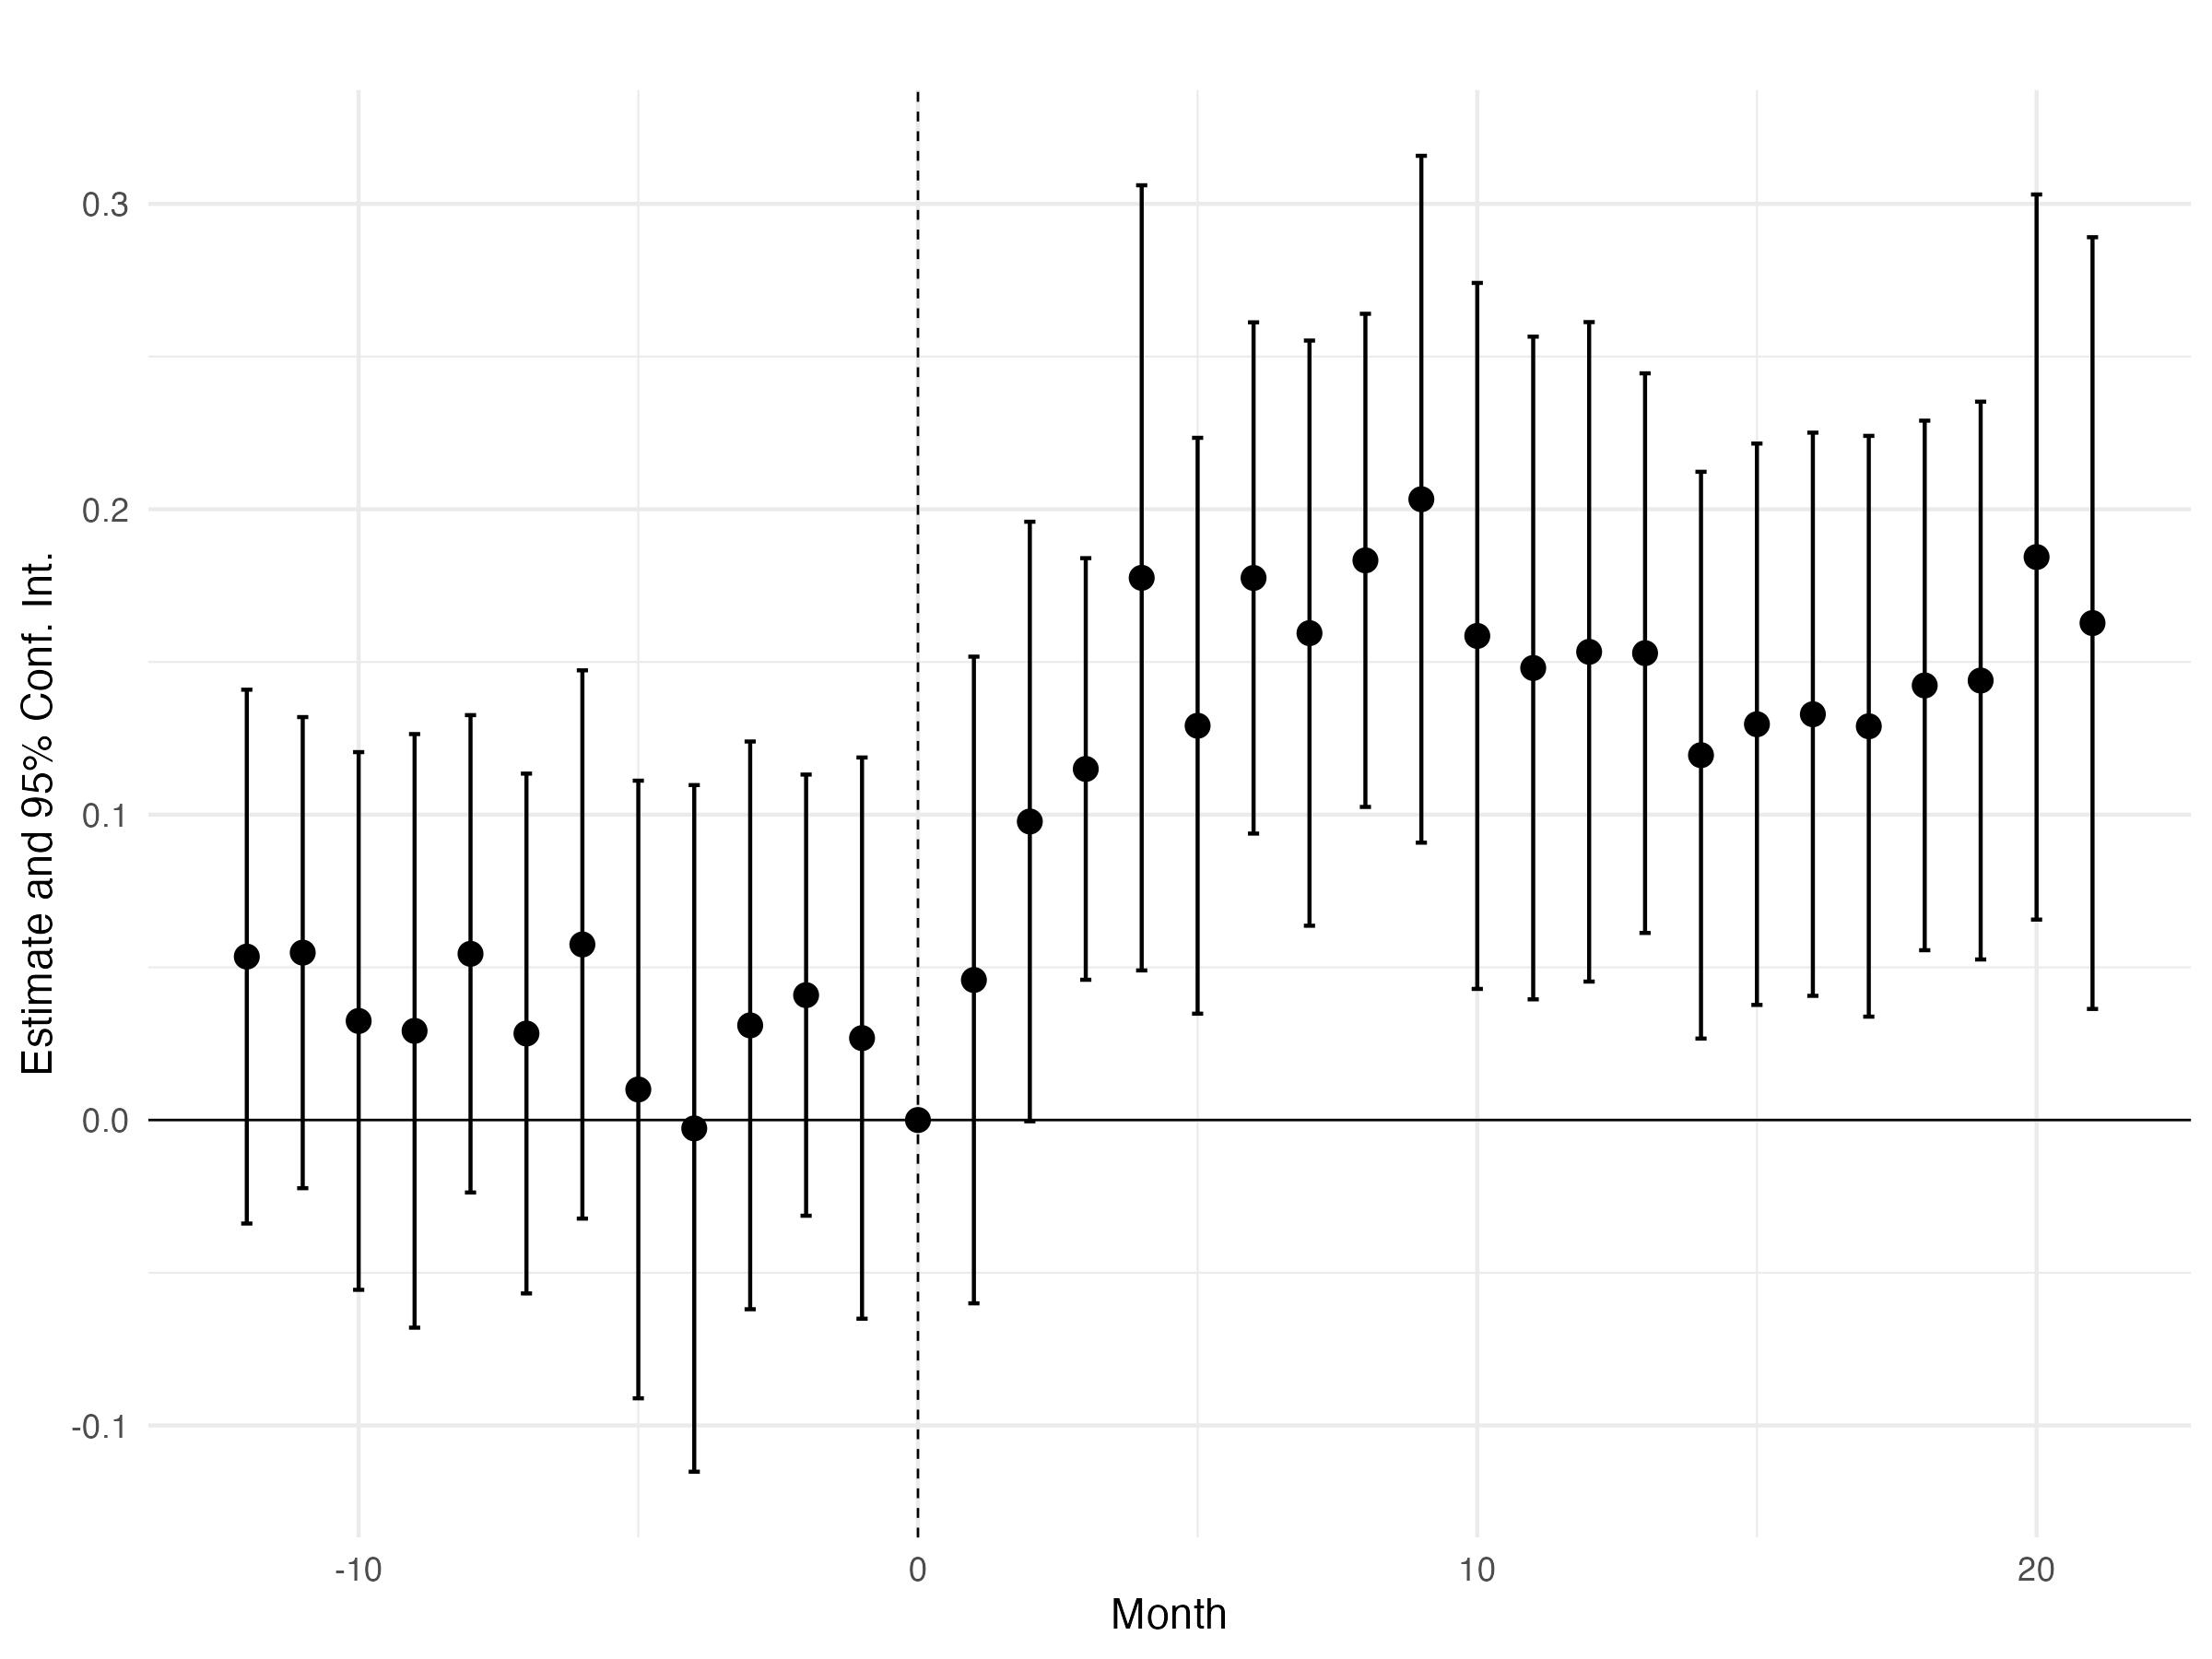
\includegraphics[scale=0.10]{Figures_Revision_2/advance_notice_es_new_wage_only.jpeg}
\vspace{-0.50cm}
\note{\scriptsize \singlespacing \textit{Notes: }  The above figure presents event-study coefficients associated with Equation \ref{eq:model_dynamic} estimated on our sample where wages are observed. Each point represents the coefficient associated with $\beta_{k}$, which is the effect of the LFW on the (log) average amount of advance notice in days, which is the average amount of advance notice for all shifts scheduled for the focal worker. Estimates are relative to the focal month of the FWL, which is indicated by the dashed vertical line. All worker-level and store-level control variables are included (See the final column of Table \ref{table:adv_notice}). The bands around estimates are 95\% confidence intervals that are constructed using standard errors that are double clustered at the store and company-year-month levels.}
\label{f:event_study_workers_wage_exists}
\end{figure}


\section{Results from Matched Samples}

\subsection{Worker-Level Results}


%% Effect on Store-Labor
\begin{singlespace}
\begin{table}[H]
\caption{Effects on Schedule Predictability (Matched Sample)}

% Created: 2025-08-05 12:32:11.110989
\begingroup
\centering
\scriptsize
\begin{tabular}{lccccc}
   \toprule
    & \multicolumn{4}{c}{log(Avg. Adv. Notice)} & Avg. Adv. Notice\\
                           & (1)           & (2)            & (3)            & (4)            & (5)\\  
   \midrule 
   LA $\times$ Post-LFW    & 0.083$^{***}$ & 0.084$^{***}$  & 0.085$^{***}$  & 0.096$^{***}$  & 1.348$^{***}$\\   
                           & (0.022)       & (0.021)        & (0.021)        & (0.021)        & (0.263)\\   
   log(Worker Mins.)              &               & -0.102$^{***}$ & -0.102$^{***}$ & -0.079$^{***}$ & -0.569$^{**}$\\   
                           &               & (0.031)        & (0.030)        & (0.026)        & (0.265)\\   
   log(Worker Shifts)             &               & 0.233$^{***}$  & 0.233$^{***}$  & 0.207$^{***}$  & 1.448$^{***}$\\   
                           &               & (0.034)        & (0.034)        & (0.030)        & (0.278)\\   
   log(Store Demand)       &               &                & -0.042         & -0.026         & -0.484\\   
                           &               &                & (0.028)        & (0.032)        & (0.441)\\   
   log(Store Labor Supply) &               &                & 0.002          & 0.027$^{*}$    & 0.252\\   
                           &               &                & (0.016)        & (0.015)        & (0.169)\\   
   log(Store Op. Mins)     &               &                & 0.089          & 0.107          & 1.562\\   
                           &               &                & (0.139)        & (0.138)        & (1.641)\\   
   log(Store Mgr. Edits)   &               &                &                & -0.129$^{***}$ & -1.526$^{***}$\\   
                           &               &                &                & (0.008)        & (0.091)\\   
    \\
   % Observations            & 90,202        & 90,202         & 90,202         & 90,202         & 90,202\\  
   Adjusted R$^2$          & 0.669         & 0.679          & 0.679          & 0.691          & 0.786\\  
    \\
   Store FEs               & $\checkmark$  & $\checkmark$   & $\checkmark$   & $\checkmark$   & $\checkmark$\\   
   Employee FEs            & $\checkmark$  & $\checkmark$   & $\checkmark$   & $\checkmark$   & $\checkmark$\\   
   Company-Month FEs       & $\checkmark$  & $\checkmark$   & $\checkmark$   & $\checkmark$   & $\checkmark$\\   
   \bottomrule
\end{tabular}
\par\endgroup



\note{\scriptsize\textit{Notes: }The estimates above correspond to our difference-in-differences estimates associated with Equation \ref{eq:model} estimated on our matched sample. This sample is constructed by first calculating pre-treatment worker-level variables (average wages, sum of total shifts, and sum of minutes worked) and store-level variables (workload minutes, labor supply, store scheduled labor minutes, store operating minutes, and managerial edits). We then implement nearest-neighbor matching with a probit distance metric that exactly matches workers on part-time status, managerial status, and company affiliation. Within these strata, it finds the closest matches based on pre-treatment characteristics, Census zip-code-level retail employment share, and log per capita income. The dependent variable is the log of average advance notice in days, calculated first at the shift-level and then averaged to the worker-month. In addition to the fixed effects described above, all regressions include the following store-level control variables: the (log) of total operating days, total operating duration in minutes, and the demand forecast. Standard errors that are double clustered at the store and company-year-month levels are presented in parentheses. *, **, and *** imply that coefficients are significant at the 10\%, 5\%, and 1\% levels, respectively. The number of observations is dropped based on the request of our data providers for our matched sample. Variable definitions are provided in Appendix \ref{sec:glossary_of_variables}.}
\label{table:adv_notice_matched}
\end{table}
\end{singlespace}

%% Effect on Store-Labor
\begin{singlespace}
\begin{table}[h]
\caption{Heterogeneous Effects on Schedule Predictability (Matched Sample)}

% Created: 2025-08-05 12:56:16.08434
\begingroup
\centering
\scriptsize
\begin{tabular}{lcccccccc}
   \toprule
    & \multicolumn{8}{c}{log(Avg. Adv. Notice)}\\
                                               & (1)           & (2)            & (3)           & (4)           & (5)           & (6)           & (7)            & (8)\\  
   \midrule 
   LA $\times$ Post-LFW                        & 0.130$^{***}$ & 0.224$^{***}$  & 0.097$^{***}$ & 0.113$^{***}$ & 0.101$^{***}$ & 0.101$^{***}$ & 0.249$^{***}$  & -0.080\\   
                                               & (0.030)       & (0.046)        & (0.021)       & (0.023)       & (0.022)       & (0.023)       & (0.049)        & (0.117)\\   
   LA $\times$ Post-LFW $\times$ Hourly Wage   &               & -0.010$^{***}$ &               &               &               &               & -0.013$^{***}$ & 0.004\\   
                                               &               & (0.003)        &               &               &               &               & (0.003)        & (0.005)\\   
   LA $\times$ Post-LFW $\times$ Part-Time     &               &                &               & -0.044$^{*}$  &               &               &                &   \\   
                                               &               &                &               & (0.023)       &               &               &                &   \\   
   LA $\times$ Post-LFW $\times$ Male          &               &                &               &               &               & 0.001         &                &   \\   
                                               &               &                &               &               &               & (0.023)       &                &   \\   
   Adjusted R$^2$                              & 0.677         & 0.679          & 0.693         & 0.694         & 0.690         & 0.690         & 0.676          & 0.699\\  
    \\
   Store FEs                                   & $\checkmark$  & $\checkmark$   & $\checkmark$  & $\checkmark$  & $\checkmark$  & $\checkmark$  & $\checkmark$   & $\checkmark$\\   
   Employee FEs                                & $\checkmark$  & $\checkmark$   & $\checkmark$  & $\checkmark$  & $\checkmark$  & $\checkmark$  & $\checkmark$   & $\checkmark$\\   
   Company-Month FEs                           & $\checkmark$  & $\checkmark$   & $\checkmark$  & $\checkmark$  & $\checkmark$  & $\checkmark$  & $\checkmark$   & $\checkmark$\\   
   \bottomrule
\end{tabular}
\par\endgroup



\note{\scriptsize\textit{Notes: }The estimates above correspond to our heterogeneous effects analyses using difference-in-differences estimates associated with Equation \ref{eq:model} at the worker-month level. The dependent variable is the log of average advance notice in days, calculated first at the shift-level and then averaged to the worker-month. The matched sample is constructed by first calculating pre-treatment worker-level variables (average wages, sum of total shifts, and sum of minutes worked) and store-level variables (workload minutes, labor supply, store operating minutes, and managerial edits). We then implement nearest-neighbor matching with a probit distance metric that exactly matches workers on part-time status, managerial status, and company affiliation. Within these strata, it finds the closest matches based on pre-treatment characteristics, Census zip-code-level retail employment share, and log per capita income. In addition to the fixed effects described above, all regressions include the following store-level control variables: the (log) of total scheduled minutes, shifts, store demand forecasts, labor supply, operating minutes, and manager edits. Standard errors that are double clustered at the store and company-year-month levels are presented in parentheses. *, **, and *** imply that coefficients are significant at the 10\%, 5\%, and 1\% levels, respectively. The number of observations is dropped based on the request of our data providers for our matched sample. Variable definitions are provided in Appendix \ref{sec:glossary_of_variables}.}
\label{table:adv_notice_het_effects_matched}
\end{table}
\end{singlespace}


\pagebreak 
\begin{singlespace}
\begin{table}[H]
\caption{Effects on Schedule Stability (Matched Sample)}

% Created: 2025-08-05 12:57:19.481503
\begingroup
\centering
\scriptsize
\begin{tabular}{lcccc}
   \toprule
                         & Shift Duration Variability & Weekly Hours Variability & Clopening Shifts    &  Unstable Start Times SHifts\\   
                         & (1)            & (2)             & (3)           & (4)\\  
   \midrule 
   LA $\times$ Post-LFW  & -0.309         & -0.017          & -0.002        & -0.006\\   
                         & (0.277)        & (0.014)         & (0.003)       & (0.010)\\   
    \\
   % Observations          & 50,627         & 50,627          & 50,627        & 50,627\\  
   Adjusted R$^2$        & 0.289          & 0.179           & 0.387         & 0.593\\  
    \\
   Store FEs             & $\checkmark$   & $\checkmark$    & $\checkmark$  & $\checkmark$\\   
   Employee FEs          & $\checkmark$   & $\checkmark$    & $\checkmark$  & $\checkmark$\\   
   Company-Month FEs     & $\checkmark$   & $\checkmark$    & $\checkmark$  & $\checkmark$\\   
   \bottomrule
\end{tabular}
\par\endgroup



\note{\textit{Notes: } \scriptsize The estimates above correspond to our difference-in-differences estimates associated with Equation \ref{eq:model} estimated on our matched sample. The matched sample is constructed by first calculating pre-treatment worker-level variables (average wages, sum of total shifts, and sum of minutes worked) and store-level variables (workload minutes, labor supply, store operating minutes, and managerial edits), then implementing nearest-neighbor matching with a probit distance metric that exactly matches workers on part-time status, managerial status, and company affiliation, and within these strata, finds the closest matches based on these pre-treatment characteristics as well as Census zip-code-level retail employment share and log per capita income. The dependent variables measure different aspects of schedule stability at the worker-month level: Column (1) is the standard deviation of shift durations normalized by total shifts, Column (2) is the standard deviation of weekly hours normalized by total shifts, Column (3) is the share of consecutive shifts with less than 10 hours of rest between them (``clopening'' shifts), and Column (4) is the share of shifts that start more than one hour earlier or later than the same day-of-week shift in the previous week (conditional on working both weeks).  In addition to the fixed effects described above, all regressions include the following store-level control variables: the (log) of total scheduled minutes, shifts, store demand forecasts, labor supply, operating minutes, and manager edits. Standard errors that are double clustered at the store and company-year-month levels are presented in parentheses. *, **, and *** imply that coefficients are significant at the 10\%, 5\%, and 1\% levels, respectively. The number of observations is dropped based on the request of our data providers for our matched sample. Variable definitions are provided in Appendix \ref{sec:glossary_of_variables}.}
\label{table:stab_regs_matched}
\end{table}
\end{singlespace}

\begin{singlespace}
\begin{table}[h]
\caption{Effects on Worker Outcomes (Matched Sample)}

% Created: 2025-08-05 12:58:20.93517
\begingroup
\centering
\scriptsize
\begin{tabular}{lccc}
   \toprule
                         & log(Worker Mins.)    & log(Worker Shifts)   & Approved Availability Change\\  
                         & (1)           & (2)           & (3)\\  
   \midrule 
   LA $\times$ Post-LFW  & 0.011         & 0.003         & 0.019\\   
                         & (0.014)       & (0.013)       & (0.043)\\   
    \\
   % Observations          & 90,202        & 90,202        & 9,224\\  
   Adjusted R$^2$        & 0.616         & 0.551         & 0.596\\  
    \\
   Store FEs             & $\checkmark$  & $\checkmark$  & $\checkmark$\\   
   Employee FEs          & $\checkmark$  & $\checkmark$  &$\checkmark$  \\  
   Company-Month FEs     & $\checkmark$  & $\checkmark$  & $\checkmark$\\   
   % Employee FEs          &               &               & $\checkmark$\\   
   \bottomrule
\end{tabular}
\par\endgroup



\note{\scriptsize \textit{Notes: } The estimates above correspond to our difference-in-differences estimates associated with Equation \ref{eq:model}. The matched sample is constructed by first calculating pre-treatment worker-level variables (average wages, sum of total shifts, and sum of minutes worked) and store-level variables (workload minutes, labor supply, store operating minutes, and managerial edits), then implementing nearest-neighbor matching with a probit distance metric that exactly matches workers on part-time status, managerial status, and company affiliation, and within these strata, finds the closest matches based on these pre-treatment characteristics as well as Census zip-code-level retail employment share and log per capita income. The dependent variables log(Mins.) and log(Shifts) are the log of total scheduled labor minutes and scheduled shifts, respectively. The underlying sample is the "full" sample as described in Section \ref{sec:data}.
In addition to the fixed effects described above, the first two regressions include the following store-level control variables: the (log) of total operating days, total operating duration in minutes, and the demand forecast. Standard errors that are double clustered at the store and company-year-month levels are presented in parentheses. *, **, and *** imply that coefficients are significant at the 10\%, 5\%, and 1\% levels, respectively. The number of observations is dropped based on the request of our data providers for our matched sample. Variable definitions are provided in Appendix \ref{sec:glossary_of_variables}.}
\label{table:worker_level_matched}
\end{table}
\end{singlespace}

\newpage 
\subsection{Store-Level Results}

\begin{singlespace}
\begin{table}[h]
\caption{Effects on Store Outcomes (Matched Sample)}

% Created: 2025-08-05 13:01:26.25275
\begingroup
\centering
\scriptsize
\begin{tabular}{lcccccc}
   \toprule
                         & PT Mins. Ratio & PT Shifts Ratio & log(Store Op. Mins) & Op. Days      & Hires         & Turnover\\  
                         & (1)            & (2)             & (3)                 & (4)           & (5)           & (6)\\  
   \midrule 
   LA $\times$ Post-LFW  & -0.011         & -0.011          & -0.017              & -0.002$^{*}$  & 0.421         & 0.307\\   
                         & (0.018)        & (0.019)         & (0.030)             & (0.001)       & (0.451)       & (0.281)\\   
    \\
   Adjusted R$^2$        & 0.723          & 0.761           & 0.996               & 0.998         & 0.288         & 0.244\\  
    \\
   Store FEs             & $\checkmark$   & $\checkmark$    & $\checkmark$        & $\checkmark$  & $\checkmark$  & $\checkmark$\\   
   Company-Month FEs     & $\checkmark$   & $\checkmark$    & $\checkmark$        & $\checkmark$  & $\checkmark$  & $\checkmark$\\   
   \bottomrule
\end{tabular}
\par\endgroup



\note{\scriptsize \textit{Notes: } The estimates above correspond to our difference-in-differences estimates associated with Equation \ref{eq:model}. The underlying sample contains the stores that result from our worker-level matching.
In addition to the fixed effects described above, all regressions include the following store-level control variables (except where the control is the dependent variable of interest): the (log) of total operating days, total operating duration in minutes, and the demand forecast. Standard errors that are double clustered at the store and company-year-month levels are presented in parentheses. *, **, and *** imply that coefficients are significant at the 10\%, 5\%, and 1\% levels, respectively. The number of observations is dropped based on the request of our data providers for our matched sample. Variable definitions are provided in Appendix \ref{sec:glossary_of_variables}.}
\label{table:store_level_matched}
\end{table}
\end{singlespace}


\end{document}
